\documentclass[a4paper]{article}

\usepackage[latin1]{inputenc} 
\usepackage{graphicx}
\usepackage{natbib} 
\usepackage{amsmath}
\usepackage{subcaption}
\usepackage[hidelinks]{hyperref}
\usepackage{listings}
\usepackage{color}
\usepackage{natbib}

\definecolor{darkblue}{rgb}{0.0, 0.0, 0.55}
\hypersetup{
    colorlinks=true,
    linkcolor=darkblue,
    filecolor=darkblue,      
    urlcolor=darkblue,
    citecolor = darkblue,
    pdftitle={Overleaf Example},
    pdfpagemode=FullScreen,
    }

\definecolor{codegreen}{rgb}{0,0.6,0}
\definecolor{codegray}{rgb}{0.5,0.5,0.5}
\definecolor{codepurple}{rgb}{0.58,0,0.82}
\definecolor{backcolour}{rgb}{0.95,0.95,0.92}
\lstdefinestyle{mystyle}{
    backgroundcolor=\color{backcolour},   
    commentstyle=\color{codegreen},
    keywordstyle=\color{magenta},
    numberstyle=\tiny\color{codegray}, 
    stringstyle=\color{codepurple},
    basicstyle=\footnotesize,
    breakatwhitespace=false,         
    breaklines=true,                 
    captionpos=b,                    
    keepspaces=true,                 
    numbers=left,                    
    numbersep=5pt,                  
    showspaces=false,                
    showstringspaces=false,
    showtabs=false, 
    tabsize=2
} 
\lstset{style=mystyle}

\newcommand{\bm}[1]{\mbox{\boldmath{$#1$}}}



\begin{document}

\begin{center}
%
\includegraphics[width=0.2\textwidth]{sw_logo} \\
\vspace{0.5 cm}
\huge{\textbf{CPlantBox Tutorial}} \\
\vspace{0.5 cm}
\normalsize
Daniel Leitner, Andrea Schnepf, et al. \\
\end{center}

\vspace{0.5 cm}

\noindent 
The following tutorial offers scripts to outline the usage of CPlantBox \citep{giraud2023cplantbox, zhou2020cplantbox} and its Python binding named \emph{plantbox}. CPlantBox was developed from CRootBox \citep{schnepf2018crootbox}, which is based on RootBox \citep{leitner2010dynamic}. CPlantBox is largely backward compatible by having the same underlying rootsystem model. For further documentation please refer to the Doxygen class documentation of the CPlantBox code.
 

\vspace{0.5 cm}

\tableofcontents

\newpage 

Progress compiling the tutorial

\begin{itemize}
 \item Section 1 finished
 \item Section 2.1-2.4 mostly finished, 2.5-2.9 in progress
 \item Section 3 no started
 \item Section 4 no started
 \item Section 5 no started 
\end{itemize}




\newpage
\section{Introduction} \label{sec:introduction}

\subsection{Installation} \label{ssec:intro_installation}
This installation guideline is for CPlantBox on Linux systems (e.g. Ubuntu). 
If on a recent Ubuntu system, the C++ compiler and python that come with the distribution are recent enough. Otherwise, please make sure you have a recent C++ compiler (e.g.   ), fortran compiler (sudo apt-get install gfortran) and python3. \\

If you wish to be able to follow the examples provided in the Jupyter Notebooks, it is recommended to install the Anaconda Python distribution: 
\begin{itemize}
\item Install curl if not yet available: \lstinline{sudo apt-get install curl}
\item Download and install Anaconda (adapt the version accordingly):\\
\lstinline{cd /tmp}\\
\lstinline{curl https://repo.anaconda.com/archive/Anaconda3-2021.11-Linux-x86_64.sh --output anaconda.sh} \\
\lstinline{bash anaconda.sh} \\
\lstinline{source ~/.bashrc}
\end{itemize}

CPlantBox can be installed using either the install script installCPlantBox.py for CPLantBox only, or installDumuxRosi\_Ubuntu.py for CPlantBox and dumux-rosi. First make sure Git ist installed, clone the CPlantBox repository, and the run the install script:
\begin{itemize}
 \item Install Git: \lstinline{sudo apt-get install git}
 \item Go to your base folder and clone repository: \lstinline{git clone https://github.com/Plant-Root-Soil-Interactions-Modelling/CPlantBox.git}
 \item Run install script: \lstinline{python3 CPlantBox/installDumuxRosi_Ubuntu.py}  
\end{itemize}

% - Install git: \\
% \\
% - Install cmake:\\
% \lstinline{sudo apt-get install cmake}\\
% - Install libboost:\\
% \lstinline{sudo apt-get install libboost-all-dev}\\
% - Install pip:\\
% \lstinline{sudo apt-get install python3-pip}\\
% - Install the python package numpy:\\
% \lstinline{pip3 install numpy}\\
% - Install the python package scipy:\\
% \lstinline{pip3 install scipy}\\
% - Install the python package matplotlib:\\
% \lstinline{pip3 install matplotlib}\footnote{Known bug in ubuntu 18.04: needs sudo apt-get install libfreetype6-dev libxft-dev installed before.}\\
% - Install the python package VTK:\\
% \lstinline {pip3 install vtk}\\
% - Install the java runtime environment:\\
% \lstinline{sudo apt-get install default-jre}\\
% - Install Paraview\\
% \lstinline{sudo apt-get install paraview}\\
% To build CPlantBox and its python shared library, move again into the CPlantBox folder and type into the console:\\
% \lstinline {cd CPlantBox}\\
% \lstinline{cmake .}\footnote{It may be necessary on your installation to check the CPlantBox/src/CMakeLists.txt file regarding required python version and out-commenting line 34.}\\
% \lstinline{make}\\
% (If building CPlantBox on the IBG-3 cluster, two lines in the file \lstinline{CPlantBox/CMakeLists.txt} need to be outcommented before:\\ 
% \lstinline{set(CMAKE_C_COMPILER "/usr/bin/gcc")}\\
% \lstinline{set(CMAKE_CXX_COMPILER "/usr/bin/g++")})\\
% 
After successfully compiling CPlantBox the Python library \emph{plantbox} should be available on your system. 


\subsection{Basic example} \label{ssec:intro_basic}
To test the installation first go to the examples \lstinline{cd tutorial/examples/} and run the following Hello World like example \lstinline{python3 intro_basic.py} to test the installation. The first example shows a CPlantBox simulation. The main steps are how to open a CPlantBox parameter file (L13), perform the simulation (L20), save the results (L23-L26), and make an interactive plot showing the results (L29). Figure \ref{fig:intro_basic} shows the expected simulation result.  

\lstinputlisting[language=Python, caption=Basic example (intro\_basic.py)]{examples/intro_basic.py} 

\noindent 
Lets revise the above code in more detail: 
\begin{itemize}
 \item[2] We add the path to find the \emph{plantbox} module.
 \item[4] Imports the CPlantBox Python library \emph{plantbox} and name it pb.
 \item[5] Imports a auxiliary script for visualization of the rootsystem with VTK and name it vp.
 \item[8] Constructs the plant object.
 \item[12] Opens an .xml containing parameters describing the structural properties of the plant by defining the seed (SeedRandomParameters), the stem (StemRandomParameters), the leaf (LeafRandomParameters) and the roots (RootRandomParameters). Alternatively, all parameter can be set or modified directly in Python. A more detailed description is given in Section \ref{sec:cplantobx}.
 \item[16] Initializes the simulation: Creates the initial stem, tap root and the base roots
 (i.e. all basal roots, and shoot borne roots that might emerge). Initializes the tropisms and passing the domain geometry, 
 and creates the elongation functions. 
 \item[20] Performs the simulation. The value 40 is the simulation time in days. If no simulation time is passed the simulation time is taken from the parameter file. Note that simulation results are independent from the time step, i.e. 40 simulate(1) calls should yield a similar result 
 as simulate(40) (due to stochasticity we cannot expect the exact same result). 
 \item[23] Saves the resulting plant geometry in the VTK Polygonal Data format (VTP) where each plant organ is repesented as a polylines. Use Paraview to visualize the results, see Section \ref{ssec:visualisation}.
 \item[25,26] If we want to visualize simulation results that are given per segment another option is to export the plant geometry segment wise. L25 creates a segment based representation of the plant geometry, and L26 saves it as VTP file.
 \item[29] Create an interactive plot (use mouse to rotate or zoom) using VTK. Per default plant 'age', 'creationTime', 'radius','organType' or 'subType' can be viusalized. The organType is 1 for the seed, 2 for root, 3 for stem, and 4 for leafs. The subType is the number of the parameter set within a organ class, i.e. the type of root, stem or leaf. You can rotate (left click) pan (right click) or zoom (mouse wheel) and save a screenshot as png file by pressing 'g', or reset view 'r', or change view by pressing 'x', 'y', 'z', and 'v'.
 \end{itemize}
  
\begin{figure}
\centering
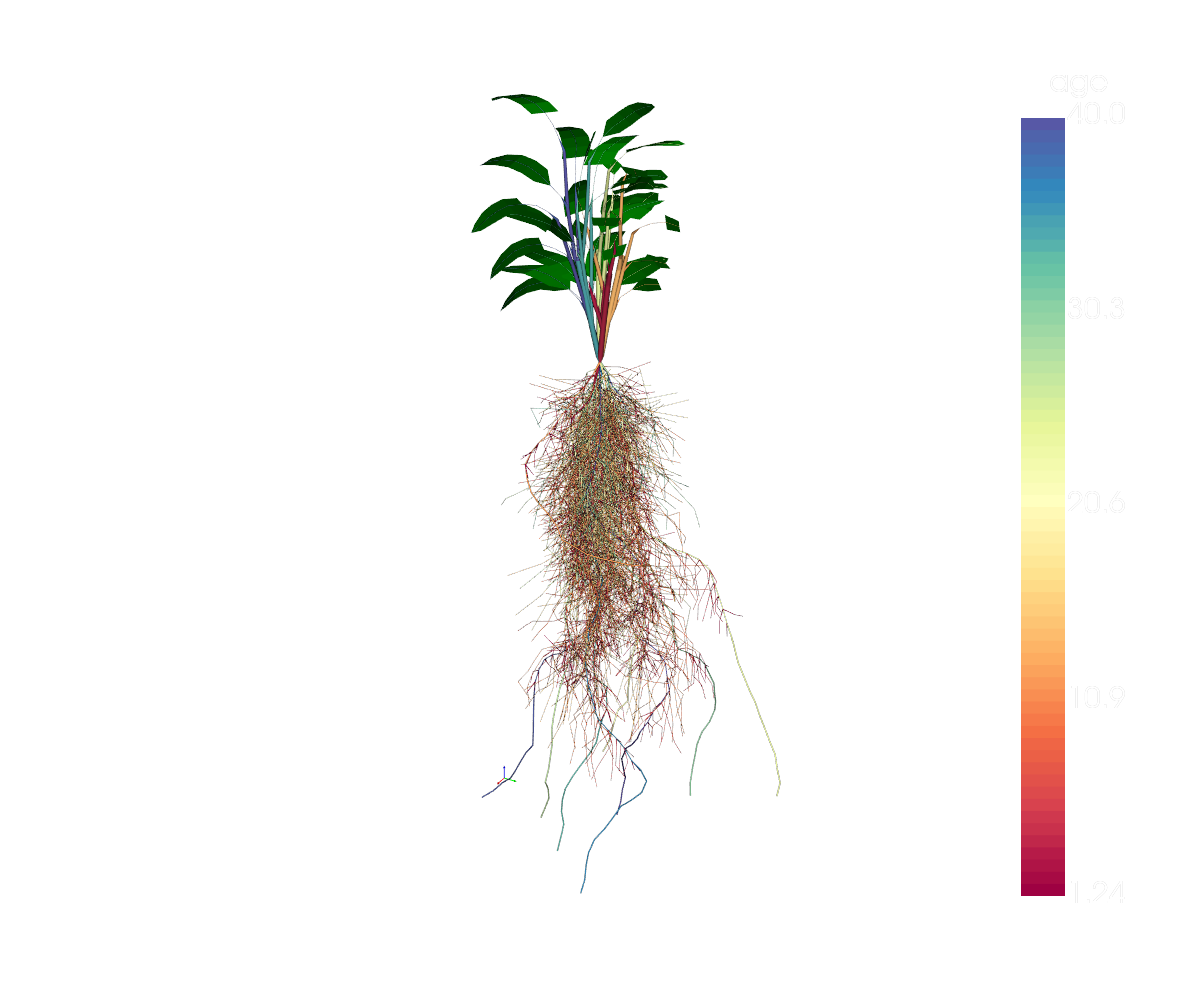
\includegraphics[width=0.5\textwidth]{figures/intro_basic.png} 
\caption{Plant after 40 days simulation time.} \label{fig:intro_basic}
\end{figure}  





\newpage
\section{Topics and Applications} \label{sec:topcis}

This section describes the usage of CPlantBox by small examples without going into details of the underlying model. A more precise description of the structural model is given in following Section \ref{sec:cplantobx}. 

\subsection{Development over time} \label{ssec:development}
The following example shows how to run the simulation in a simulation loop. This is important if we want to couple the model and implement feedbacks, or as in this case, if we want to retrieve information over time. The following script shows how to calculate the organ lengths over time. 

\lstinputlisting[language=Python, caption=Organ development over time]{examples/topics_development.py}

\begin{itemize}
\item[8-13] Sets up the simulation.

\item[15-17] Defines the simulation time, time step, and the resulting number of simulate(dt) calls. 

\item[23-36] The simulation loop executes the simulation for a single time step L26. After each simulation step, we retrieve the organ type, the sub type, and the length of each organ (L28-30). It is possible to access all root random parameters and resulting realisations using plant.getParameter. In C++ the class functions are defined in Plant::getParameter, Organ::getParameter. In L31-36 we sum up specific organ lengths by boolean array indexing.

\item[38-47] Creates Figure \ref{fig:topics_development}.

\end{itemize}


Next we show how retrieve root tip and root base positions from a simulation. Each organ is represented by a polyline, which is a list of points connected by segments. We use this polyline to plot the base (first node of the polyline) and the tip (last node of the polyline). 

\lstinputlisting[language=Python, caption=Organ tips and bases over time]{examples/topics_development2.py}

\begin{itemize}

\item[8-17] Sets up the simulation and simulation loop as before.

\item[21-28] L23 performs the simulation for a single time step. First we retrieve all organs as polylines L25, where organ tips are the last nodes of the polylines L27, and organ bases are the first nodes L28. Organs that have not started to emerge have only 1 node, and are not retrieved by getPolylines().

\item[30,31] Convert the lists to numpy array for indexing.

\item[33-41] Creates Figure \ref{fig:topics_development2}. In CPlantBox roots are growing with a negative exponential growth rate, i.e. growth becomes slower towards the root reaching its maximal length. Therefore, the node density becomes higher towards the root tips. 

\end{itemize}

\begin{figure}
\begin{subfigure}[c]{0.5\textwidth}
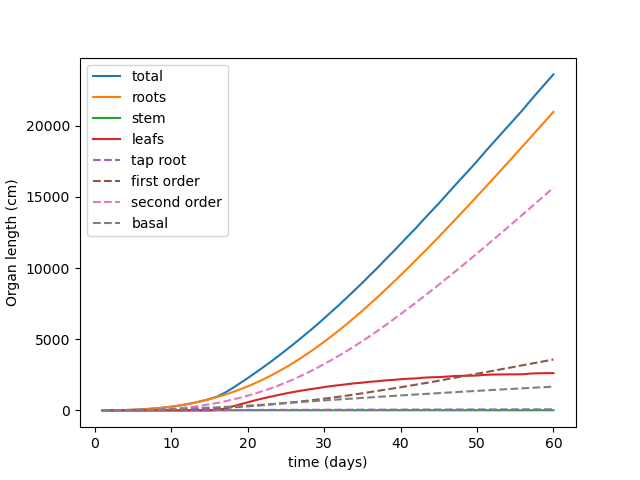
\includegraphics[width=0.99\textwidth]{examples/results/topics_development.png}
\subcaption{Total organ lengths versus time} \label{fig:topics_development}
\end{subfigure}
\begin{subfigure}[c]{0.5\textwidth}
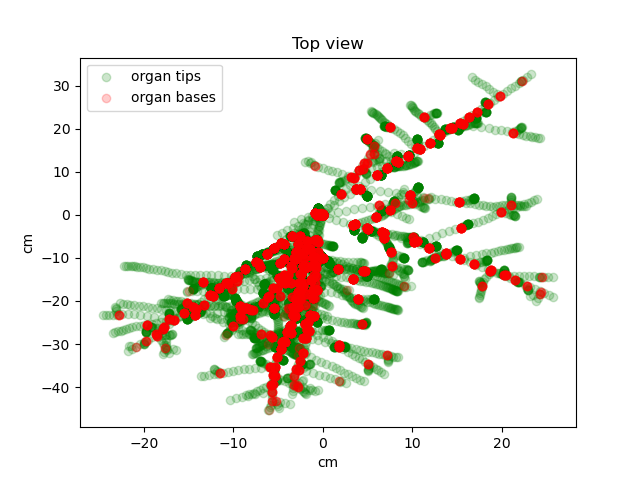
\includegraphics[width=0.99\textwidth]{examples/results/topics_development2.png}
\subcaption{Top view of the organ tip and bases} \label{fig:topics_development2}
\end{subfigure}
\caption{Plant development over time} 
\end{figure}




\subsection{How to virtually mimic experiments} \label{ssec:virtual}
In order to mimic experimental settings we can confine root growth by containers, or we can implement obstacles hindering root growth. Furthermore, periodic domains can be used to mimic field conditions. In CPlantBox the domain geometry is represented in a mesh free way using signed distance functions (SDF). A SDF returns the distance of a point to its closest boundary, with negative sign if it lies inside of the domain, and a positive if the point is outside. CPlantBox has auxilliary functions for creating simple domains, which is shown in the following example.

\subsubsection*{Growth in a container}

We show two examples where the plants root system grows confined by two types of containers 
(by a cylindrical container or a rectangular rhizotron). 

\lstinputlisting[language=Python, caption=Root growth in a container (topics\_virtual.py)]{examples/topics_virtual.py}

The geometry is first created by constructing some specialization of the class SignedDistanceFunction, 
and is passed to the root system by the method setGeometry: 
\begin{itemize}
 \item[9-11] choose t
 he parameter input file
 \item[14] Construct a cylindrical container. 
 \item[16] Construct a rhizotron.
 \item[20] Pick one of the two geometries. Note that it is important to call plant.setGeometry() before plant.initialize().
 \item[23,24] Initializes and simualtes for 40 days.
 \item[27] Exports the plant structure geometry (without the soil domain geometry).
 \item[31] Its possible to save the soil domain geometry as Paraview Python script for visualization (and debugging), see Figure \ref{fig:topics_virtual}. Run this script in Paraview by Tools$\rightarrow$Python Shell, Run Script. 
\item[34] Interactive VTK plot. The geometric boundaries can currently not be visualized in the interactive rendering. This could be achieved in VTK by creating an iso-surface of the implicit geometry given by the SDF. visualised. 
\end{itemize}

\begin{figure}
\begin{subfigure}[c]{0.5\textwidth}
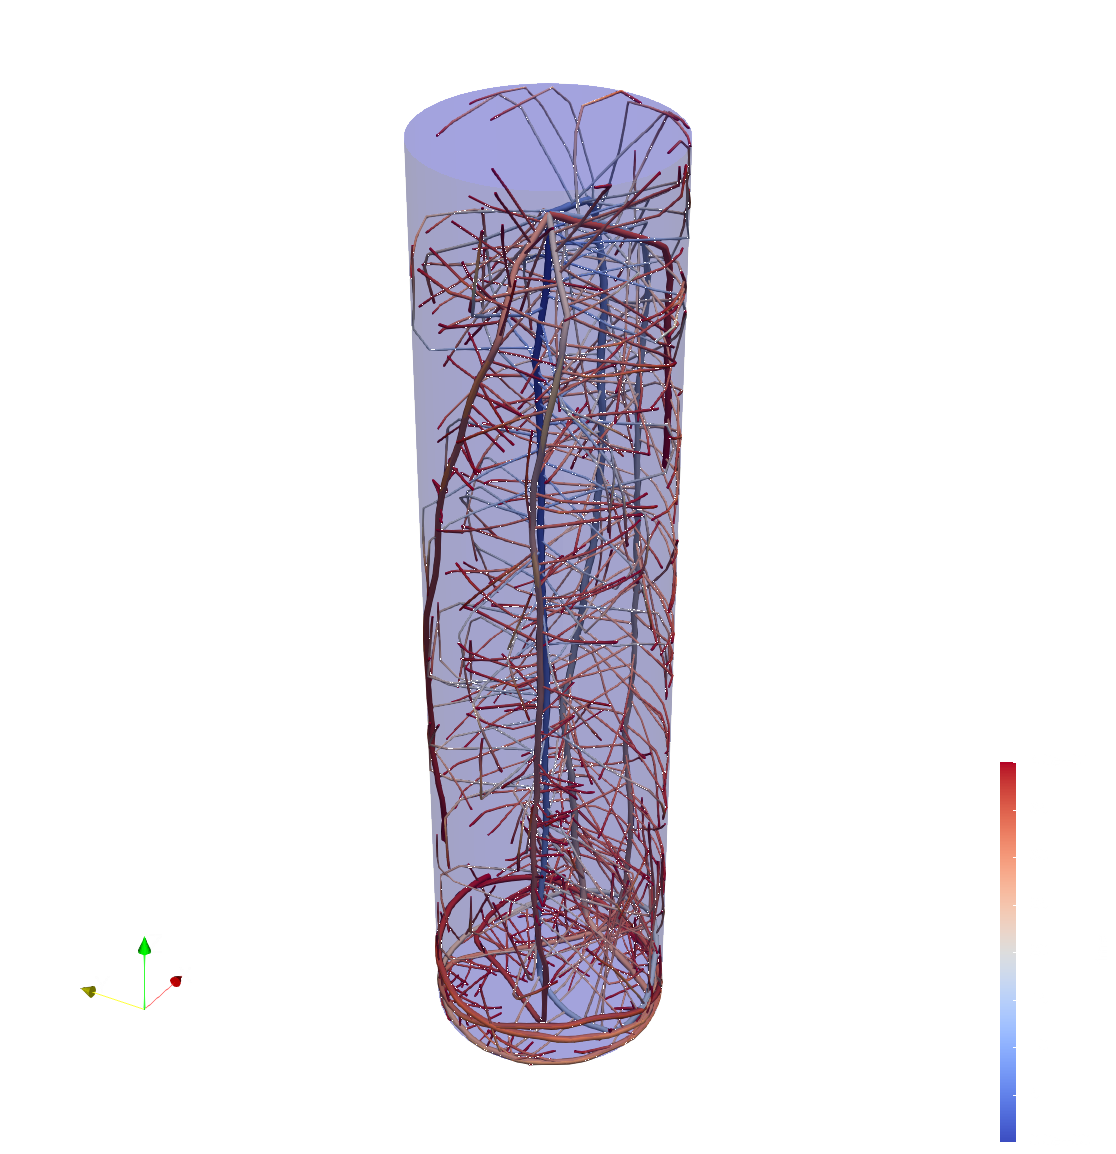
\includegraphics[width=0.99\textwidth]{figures/topics_virtual_a.png}
\subcaption{Confined by a cylinder (colour represent root age)} 
\end{subfigure}
\begin{subfigure}[c]{0.5\textwidth}
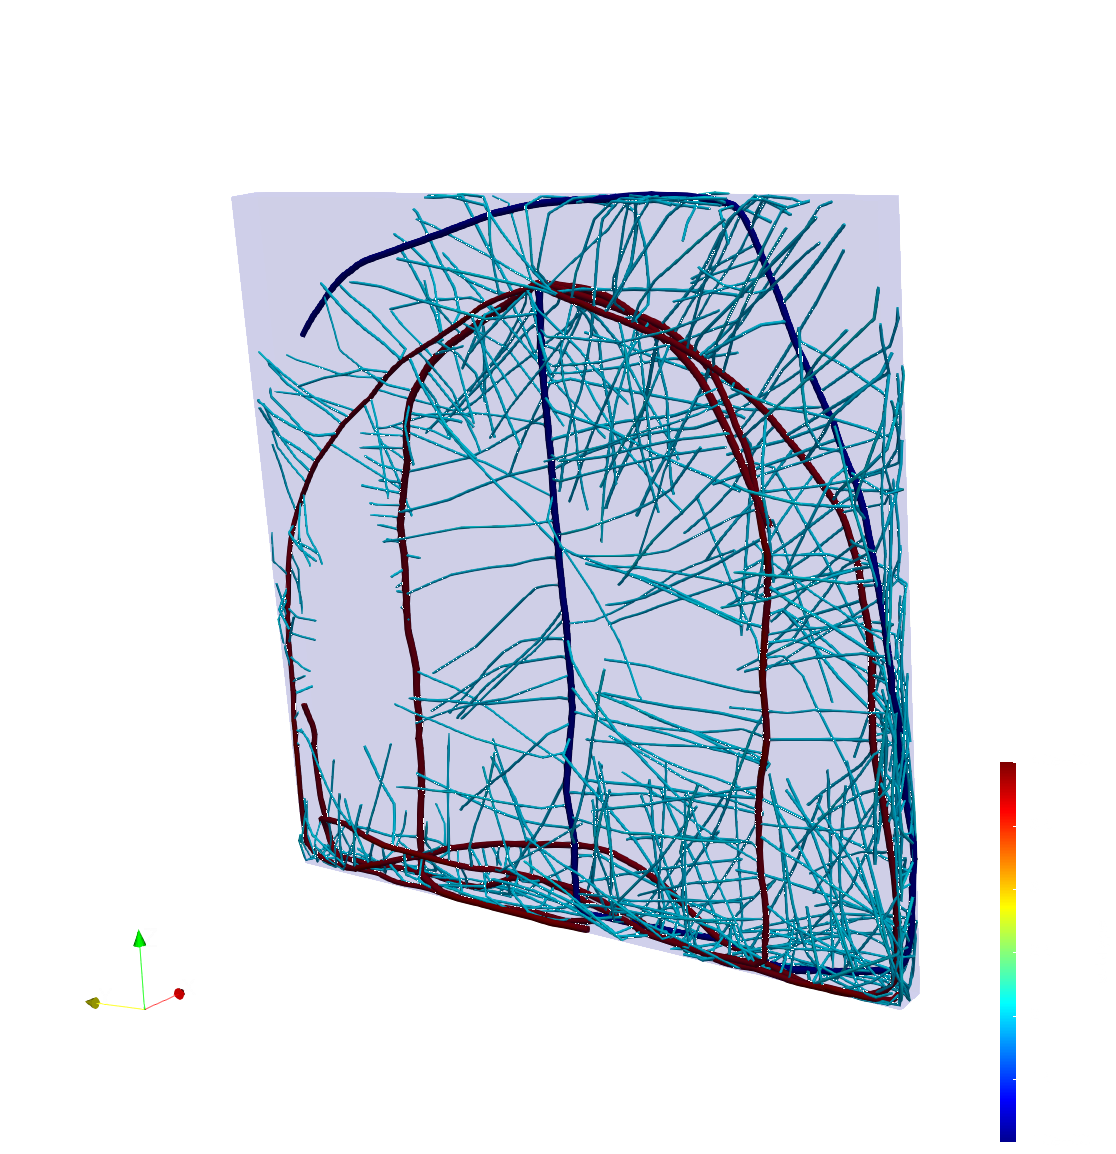
\includegraphics[width=0.99\textwidth]{figures/topics_virtual_b.png}
\subcaption{Confined by a rhizotron (colour represent root type)} 
\end{subfigure}
\caption{ParaView visualizations of results.} \label{fig:topics_virtual}
\end{figure}

Next, we show how to build more complex container geometries using SDF. 


\subsubsection*{Complex containers using SDF with set operations}

In the following example we create geometries that we might encounter in experiments. 
First, we show how to rotate a rhizotron (e.g. to see more roots at the wall due to gravitropism). 
Second, we create a split box experiment, and furthermore, an example where rhizotubes act as obstacles.The following examples demonstrates how to build a complex geometry using rotations, translations and set operations on the SDF.

\lstinputlisting[language=Python, caption=Root growth in more complex containers (topics\_virtual2.py)]{examples/topics_virtual2.py}

\begin{itemize}
\item[14-19] Definition of a rotated rhizotron, see Figure \ref{fig:topics_virtual2_a}: 
L15 creates the flat container with a small height, this container is then rotated and translated into the desired position. L16 is the location of the plant seed within the unrotated rhizotron. L17 defines the rotational matrix rotating around the x-axis. In L18 the seed position is rotated. Finally, in L21 the rhizotron is rotated and translated so that the seed location is moved to the origin. 
\item[21-30] Definition of of a split box, see Figure \ref{fig:topics_virtual2_b}: 
The split box is composed of a left box, a right box, and a top box connecting left and right. 
In L30 the geometry is defined by the set operation union of the three compartments. 
\item[33] Pick one of the three geometries for your simulation.
\item[39] Also more complex geometries can be visualized by the Paraview script, 
however, set operations are not really performed, only the involved geometries are visualized.
\item[40] We cannot visualize the container geometry in the interactive rendering, but only the resulting root system. 
\end{itemize}

\begin{figure}
\begin{subfigure}[c]{0.49\textwidth}
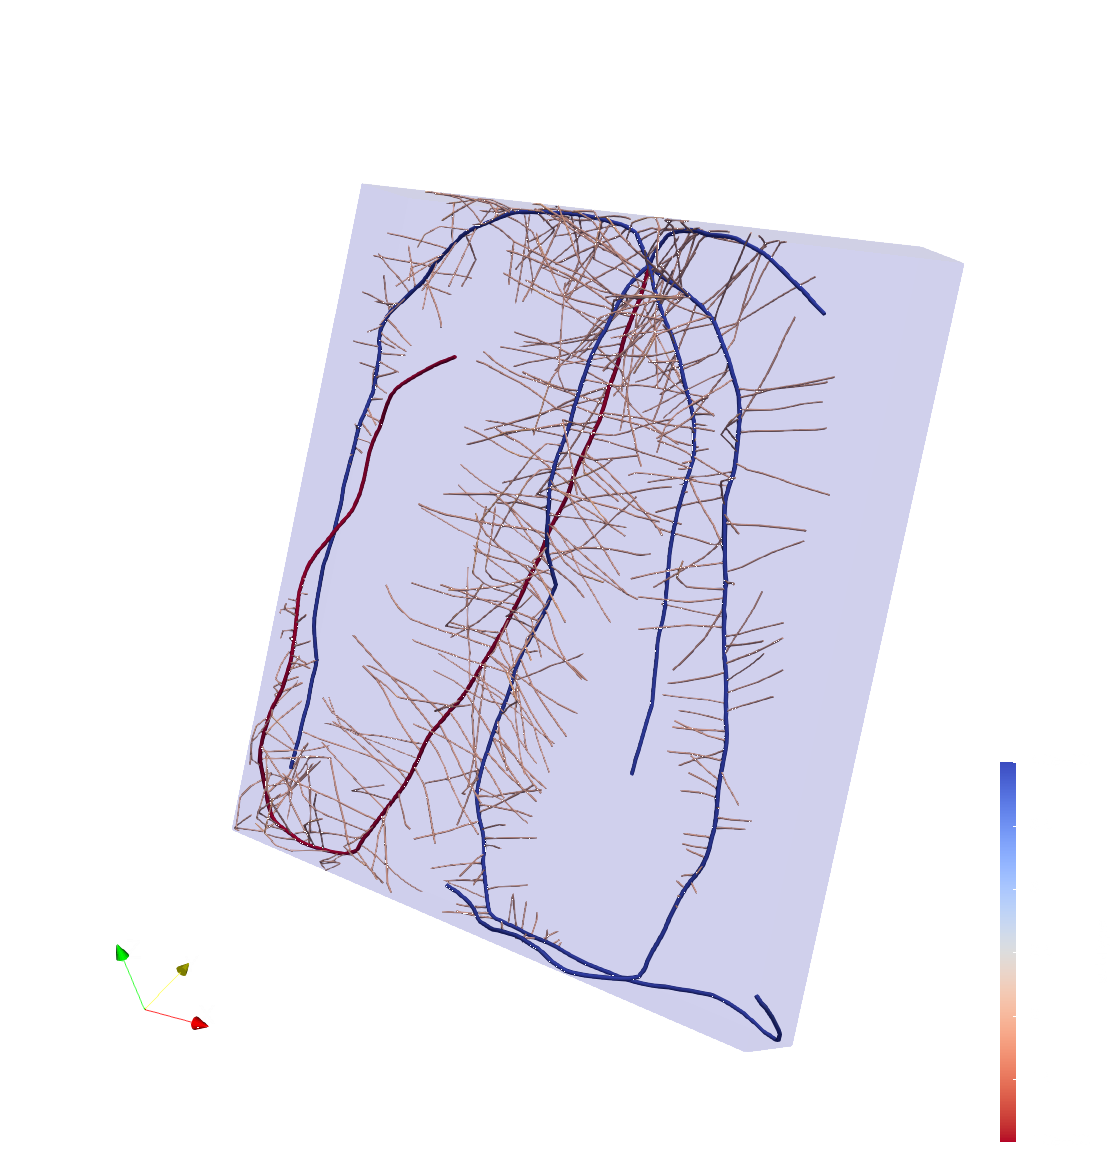
\includegraphics[width=0.99\textwidth]{figures/topics_virtual2_a.png} 
\subcaption{Rotated rhizotron} \label{fig:topics_virtual2_a}
\end{subfigure}
\begin{subfigure}[c]{0.49\textwidth}
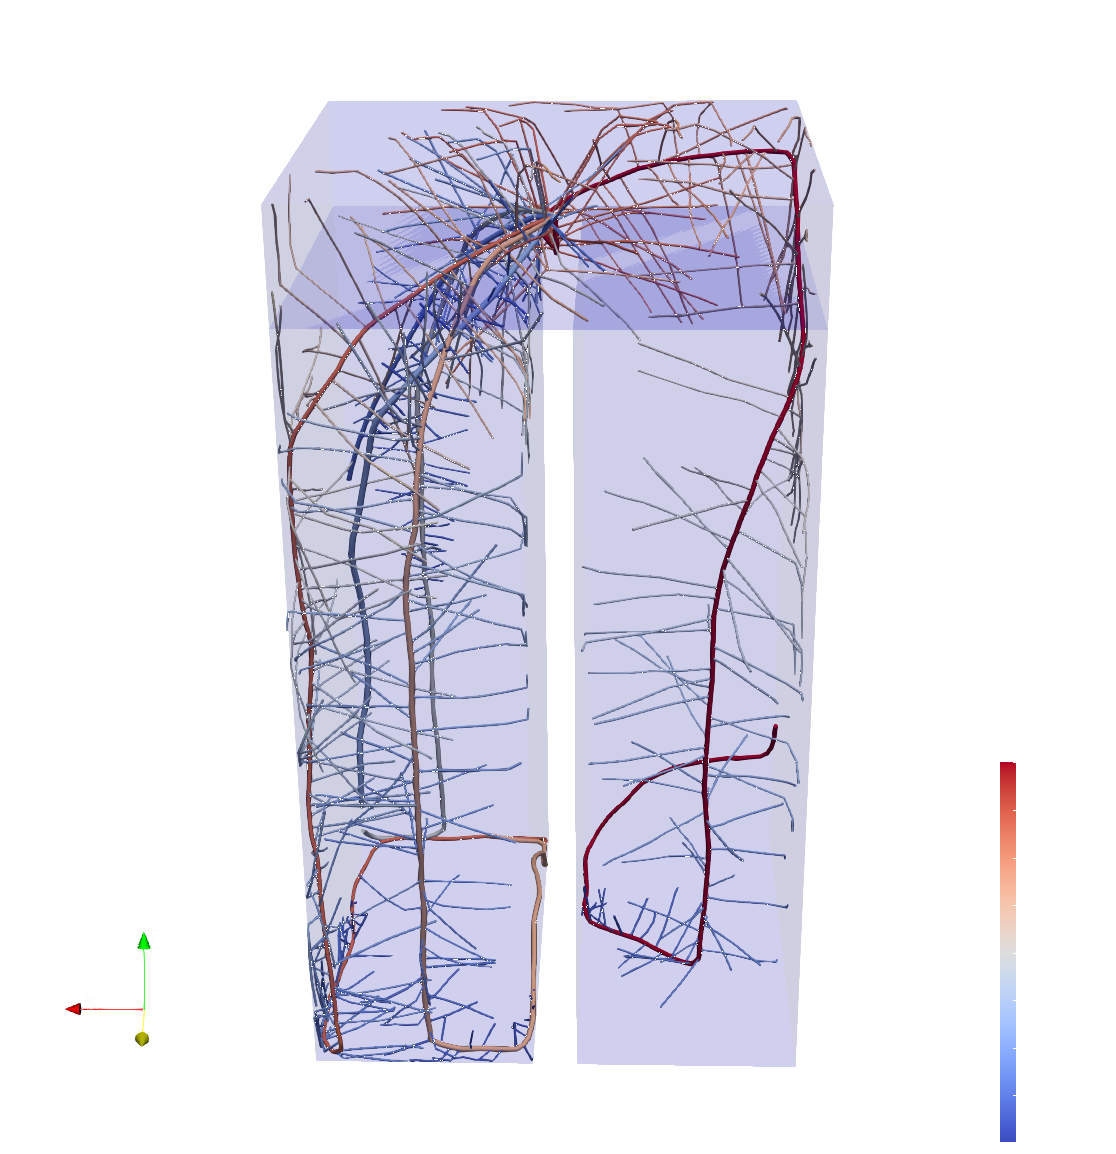
\includegraphics[width=0.99\textwidth]{figures/topics_virtual2_b.png} 
\subcaption{Split box experiment} \label{fig:topics_virtual2_b}
\end{subfigure}
\caption{Complex container geometries described by SDF and set operations.}
\end{figure}

\subsubsection*{Obstacles using SDF}

We can also use set operations to create obstacles. The following example shows a rhizotube camera setup, where transparent tubes are used to analyse root growth. We can mimic this setup by defining tubes that act as an obstacle to the growing roots. The following code is exactly the same as before, but with another geometry: 

\lstinputlisting[language=Python, caption=Experimental setup with rhizotubes (topics\_virtual3)]{examples/topics_virtual3.py}

\begin{itemize}
\item[18-28] Definition of rhizotubes as obstacles, see Figure \ref{fig:topics_virtual3}: L14 is the surrounding box, L15 a single rhizotube, that is rotated around the y-axis in L16. L21-L26 create a list of rhizotubes at different locations that mimics the experimental setup.  L27 and L28 compose the final geometry by to set operation, first a union of all tubes, and then cut them out the surrounding box by taking the difference. 
\end{itemize}

\begin{figure}
\centering
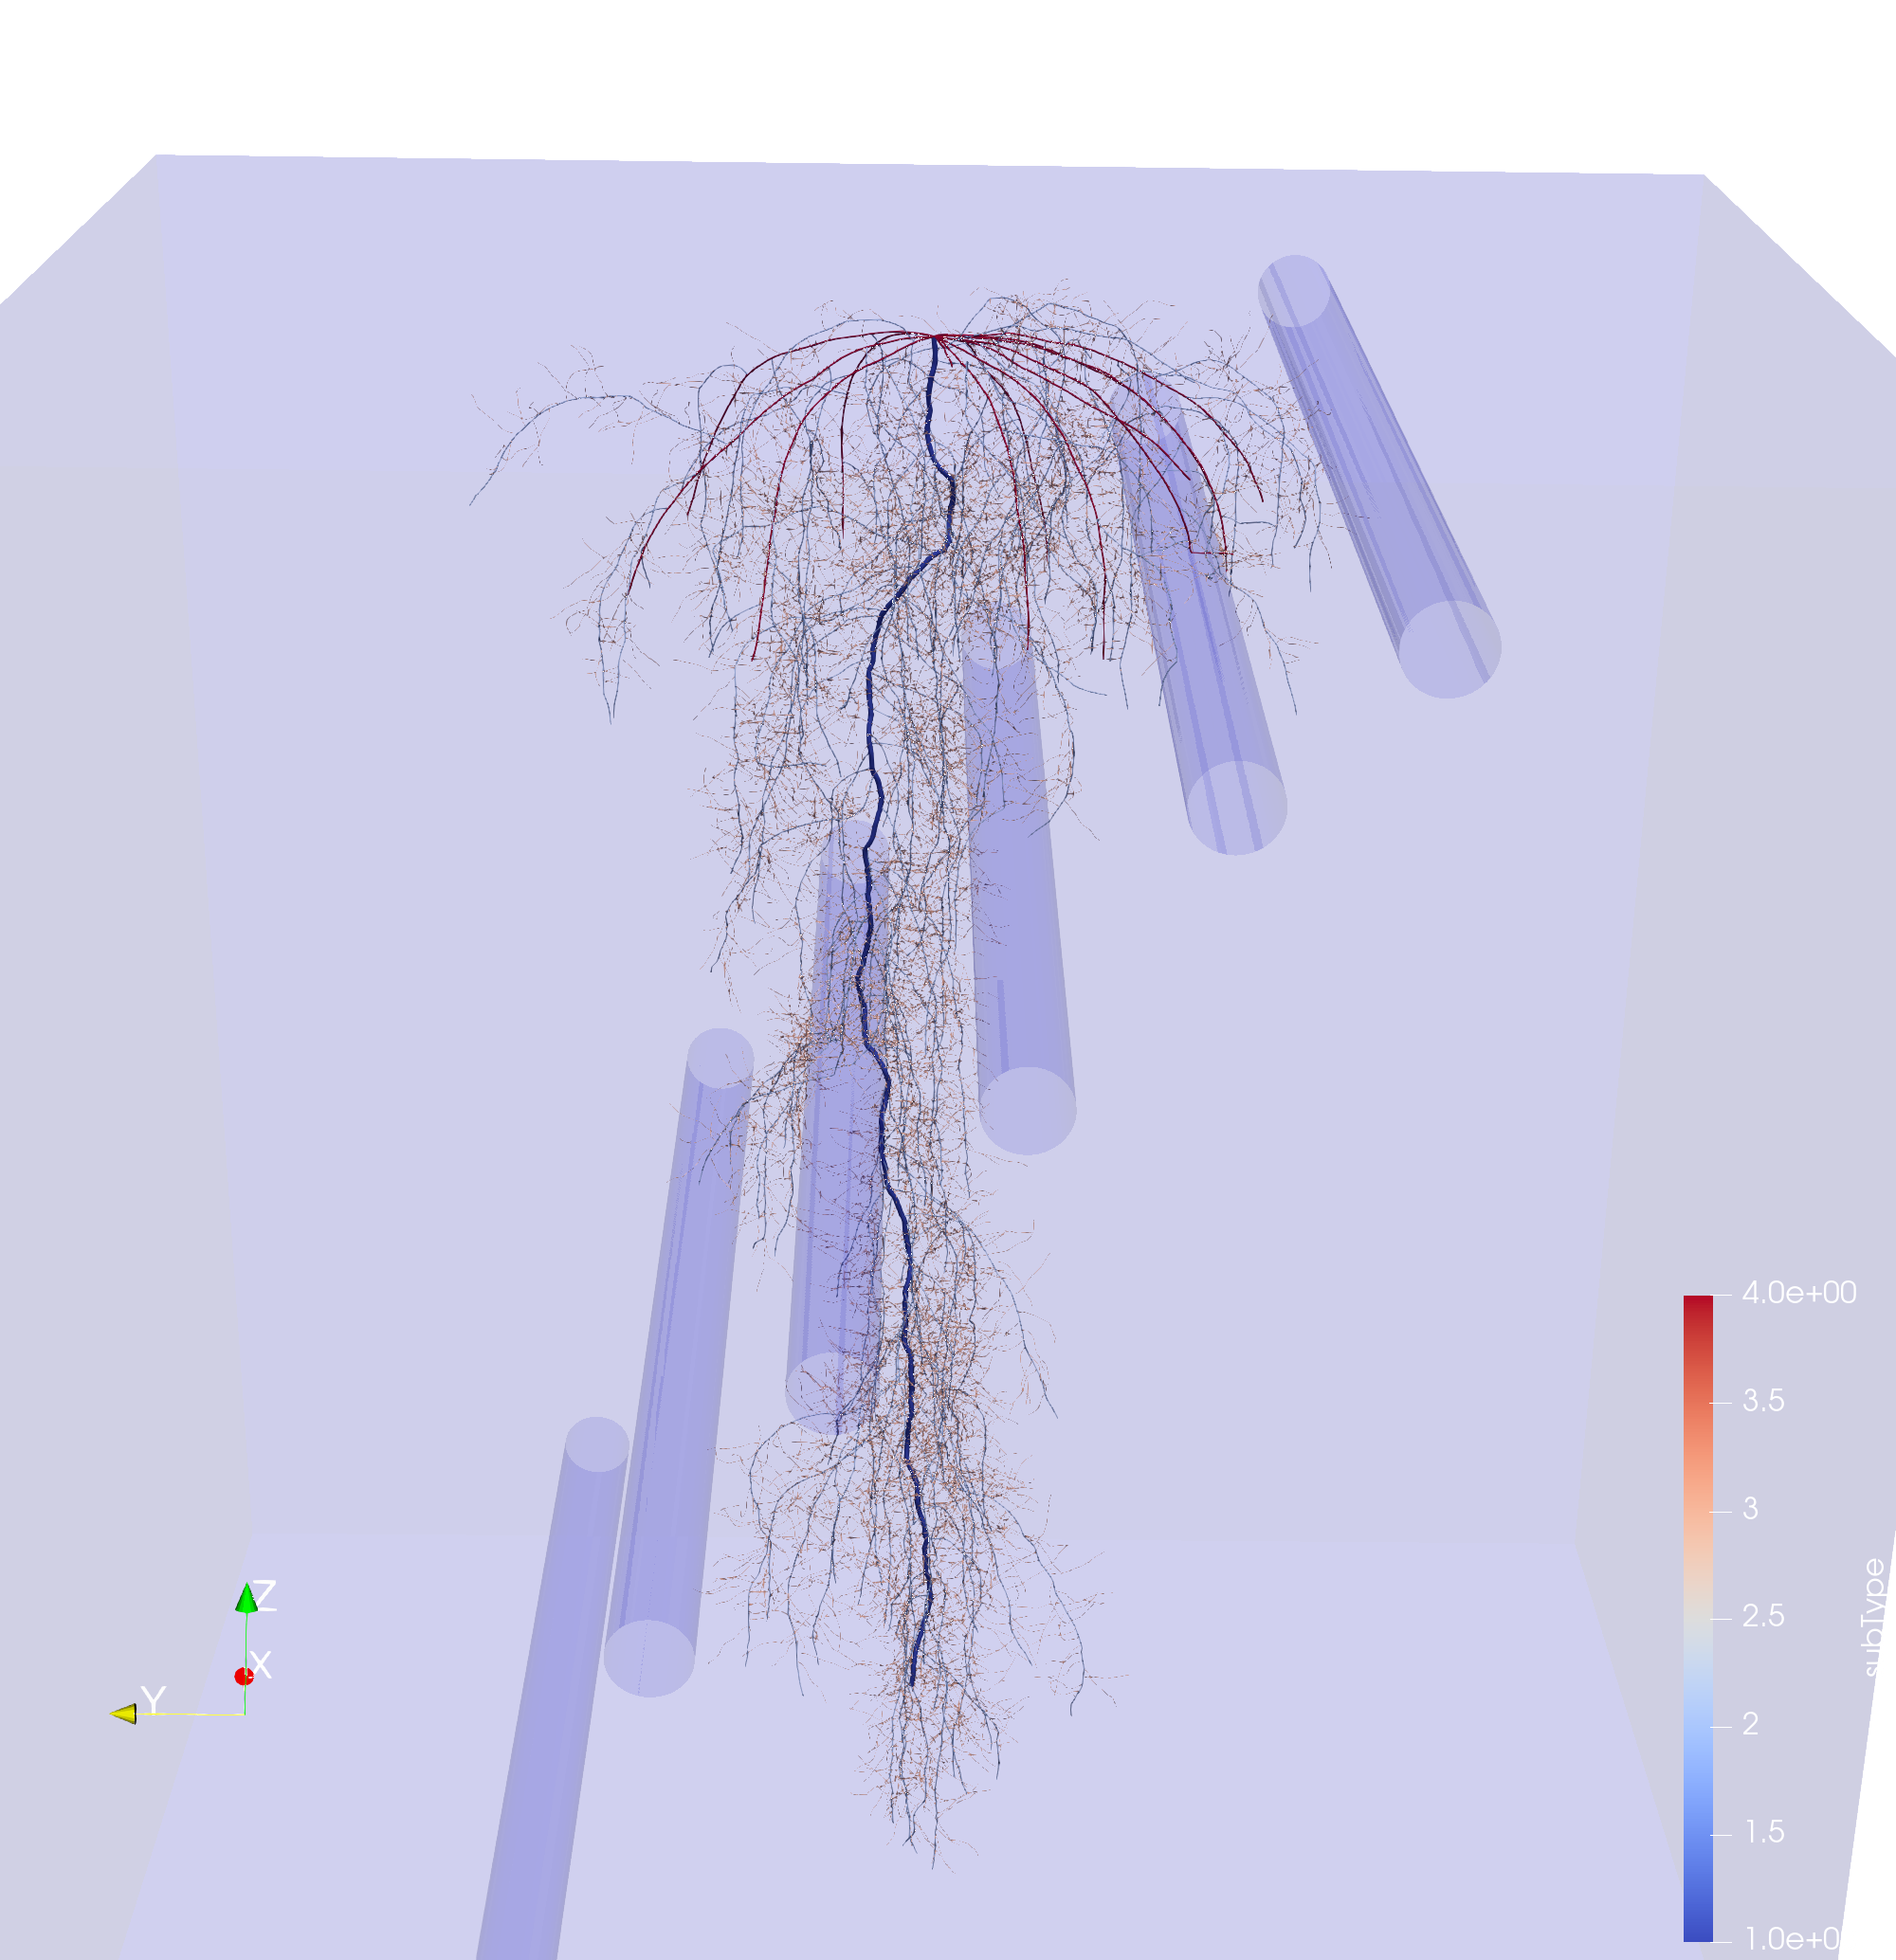
\includegraphics[width=0.7\textwidth]{figures/topics_virtual3.png}
\caption{Rhizotubes act as obstacles to the root system} \label{fig:topics_virtual3}
\end{figure}

\subsubsection*{Multiple root systems}

Its possible to simulate multiple root systems. In the following we show a small plot scale simulation.

\lstinputlisting[language=Python, caption=Multiple root systems (topics\_virtual4.py)]{examples/topics_virtual4.py}

\begin{itemize}
\item[11,12] Set the number of columns and rows of the plot, and the distance between the root systems.
\item[15-24] Creates the root systems, and puts them into a list \texttt{all}. L20 retrieves the plant seed, and L21 sets a new seed position. 
\item[26,27] Simulate all root systems 
\item[30-37] Saves each individual root systems, and additionally, saves all root systems into a single file. 
Therefore, we create an SegmentAnalyser (see Section \ref{ssec:postprocessing}) object in L30 and merge all organ segments into it L34,  and finally export the single file L37. The resulting geometry is shown in Figure \ref{fig:topics_virtual4}.
\end{itemize}

\begin{figure}
\centering
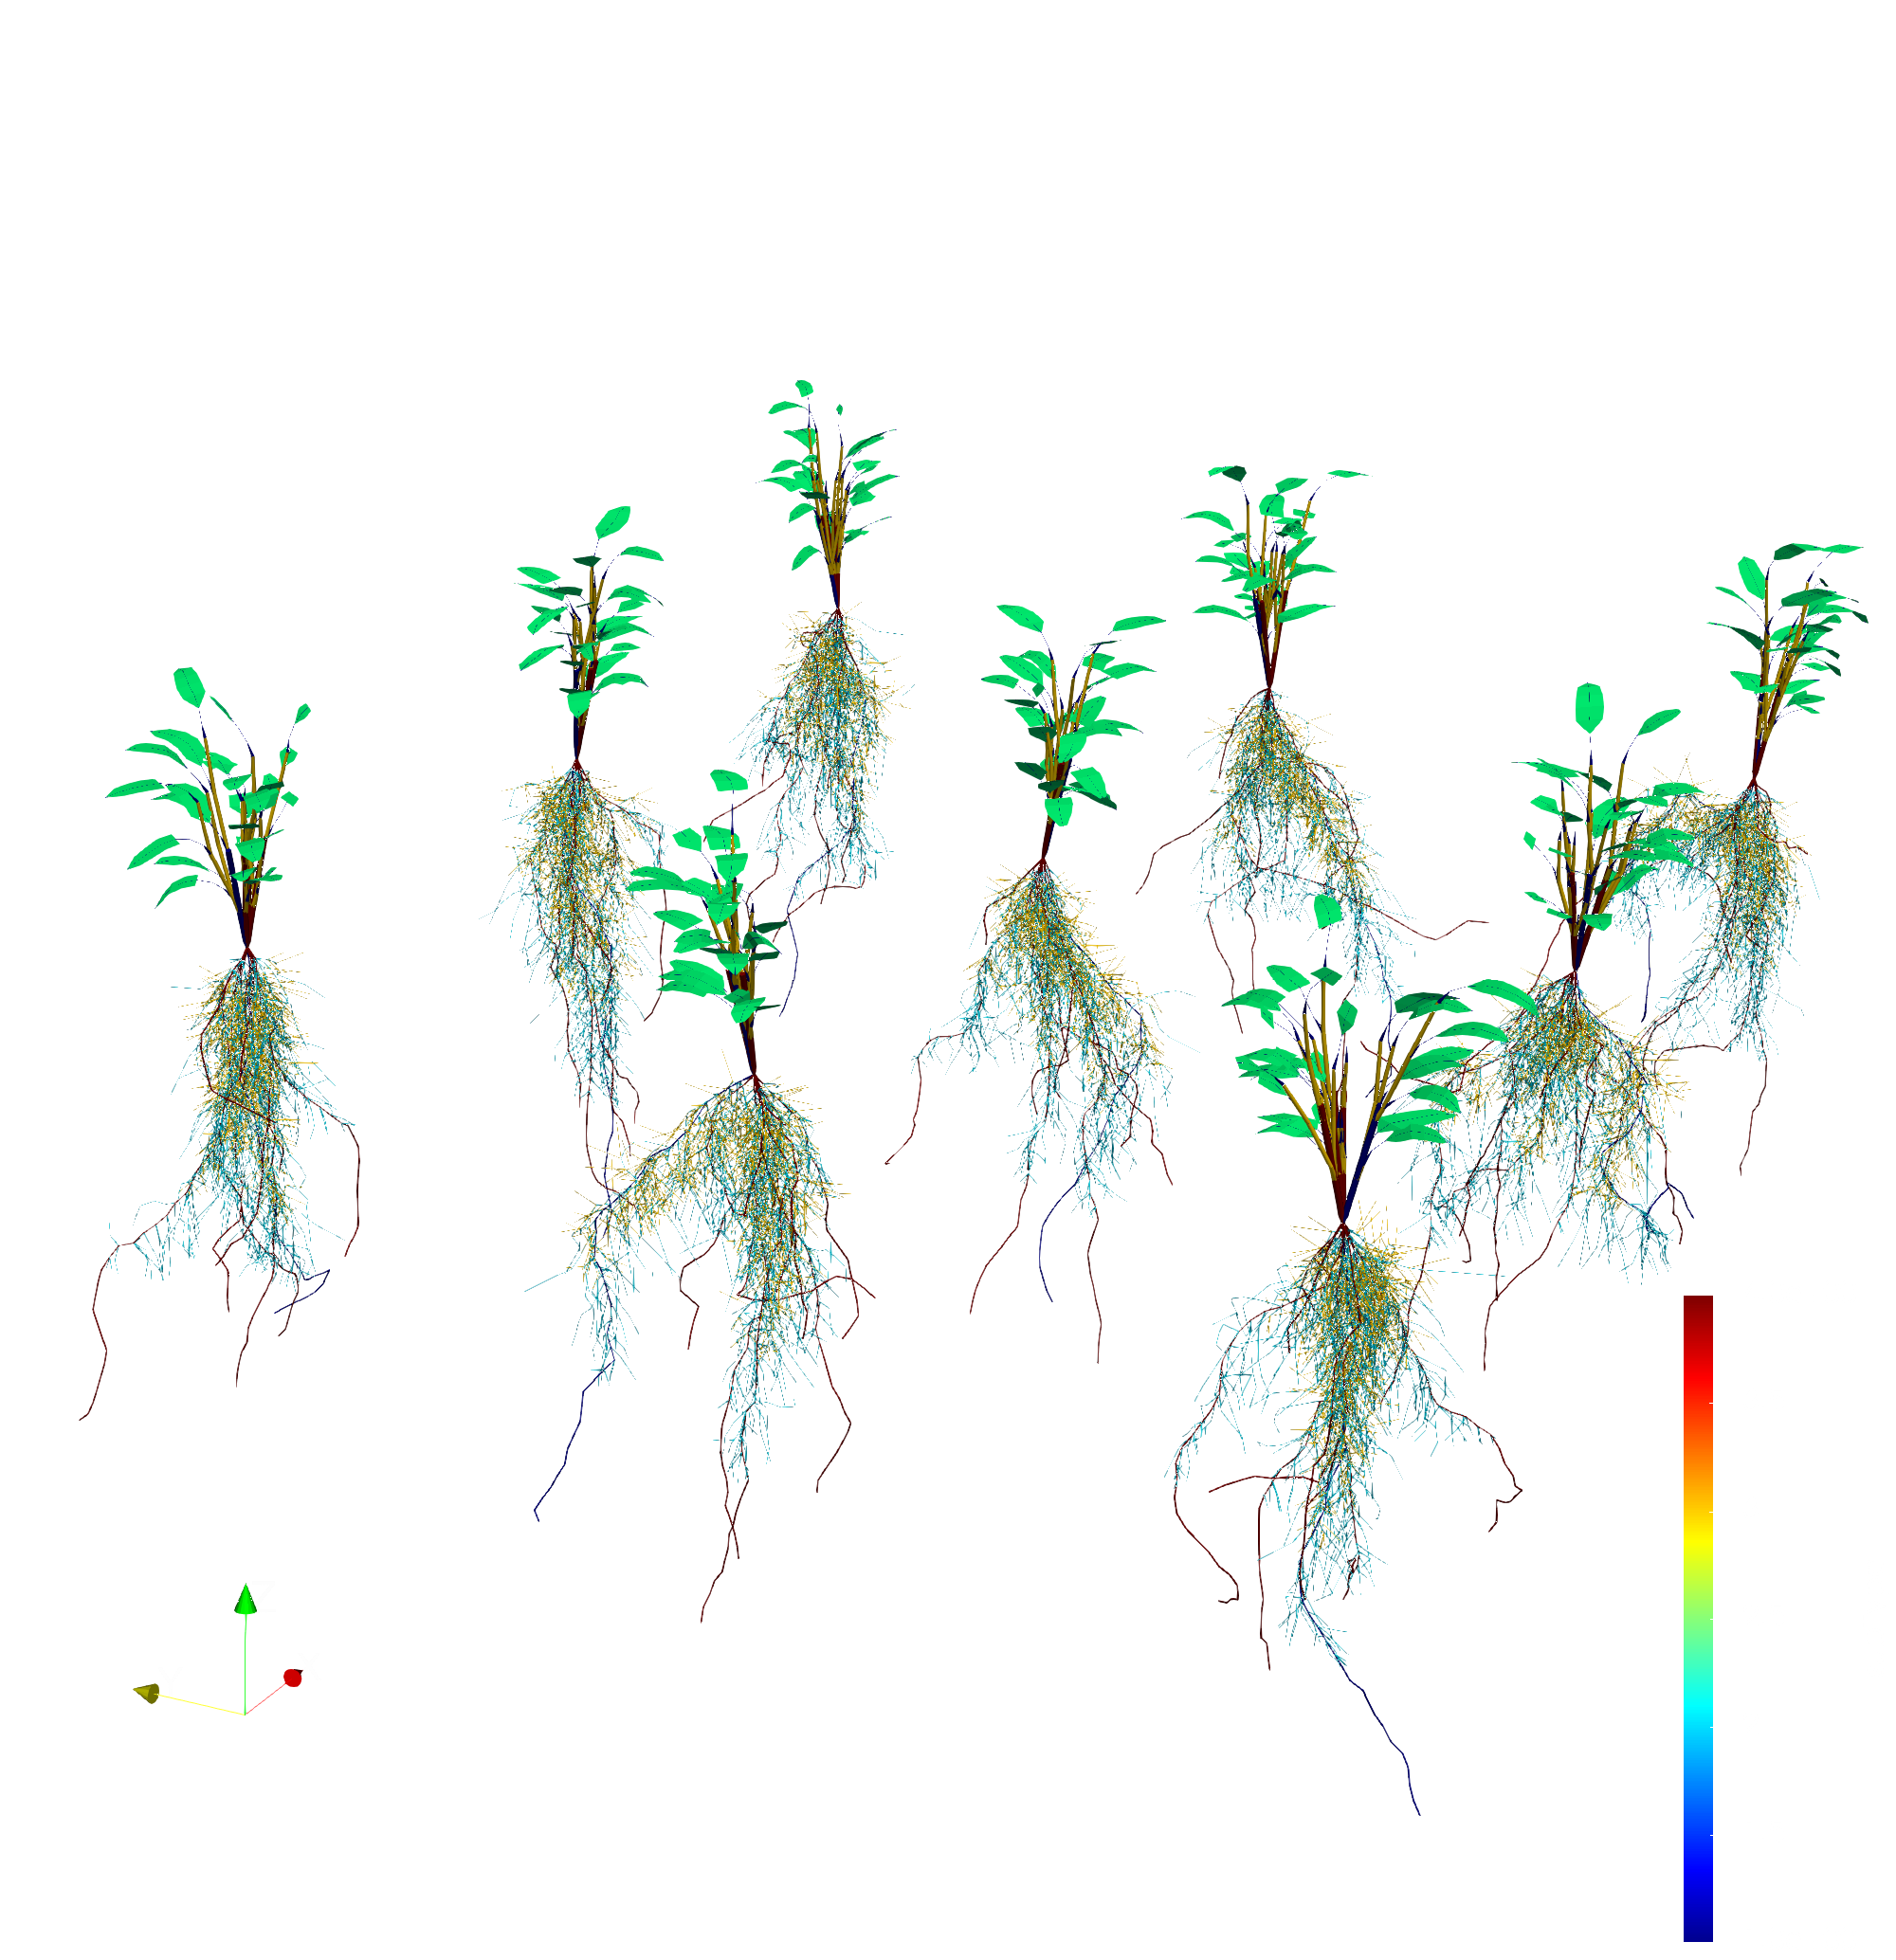
\includegraphics[width=0.7\textwidth]{figures/topics_virtual4.png}
\caption{ParaView visualization of multiple root systems} \label{fig:topics_virtual4}
\end{figure}


\subsubsection*{Periodic domains}

If we consider only one plant type we often simplify field scale simulations to a single plant simulation with a periodic domain where the domain length and width is determined by planting density and inter-row density. We can analyse the root geometry mapped to a periodic grid using SegmentAnalyser::mapPeriodic, see Section \ref{ssec:postprocessing}. For coupling a root system with a periodic macroscopic soil model an unimpeded single root system is calculated and mapped to the periodic domain by the root to soil mapping function, see Section \ref{ssec:mapped}.





\subsection{Postprocessing} \label{ssec:postprocessing}
The class SegmentAnalyser offers post-processing methods per organ segment. The advantage is that we can do distributions or densities, and that we can analyse the segments within any geometry by cropping the overall geometry to a region of interest. While the class SegmentAnalyser was designed for analysing roots most functionallity works also for the above plant part. 

\subsubsection*{Root surface densities}

We start with a small example plotting the root surface densities of a root system versus root depth.

\lstinputlisting[language=Python, caption= Calculating root surface densities in a soil column]{examples/topics_postprocessing.py}

\begin{itemize}
\item[9-12] Pick a plant or root system.
\item[14-16] Depth is the length of the soil column (into z-direction), layers the number of vertical soil layers, where the root surfaces are accumulated, and runs is the number of simulation runs. 
\item[18] Creates a confing geometry.
\item[20-26] Performs the simulations for $runs$ times. L26 creates a distribution of a parameter (name) over a vertical range (bot, top). The data are accumulated in each layer, segments are either cut (exact = True) or accumulated by their mid point (exact = False). 
\item[28,29] In order to calculate a root surface density from the summed up surface, we need to define a soil volume. The vertical height is the layer length, length and width (here 10 cm), can be determined by planting width, or by a confining geometry. 
\item[30-31] Calculates the densities mean and the standard error. 
\item[33-42] Prepares the plot (see Figure \ref{fig:topics_postprocessing}).
\end{itemize}

\begin{figure}
\centering
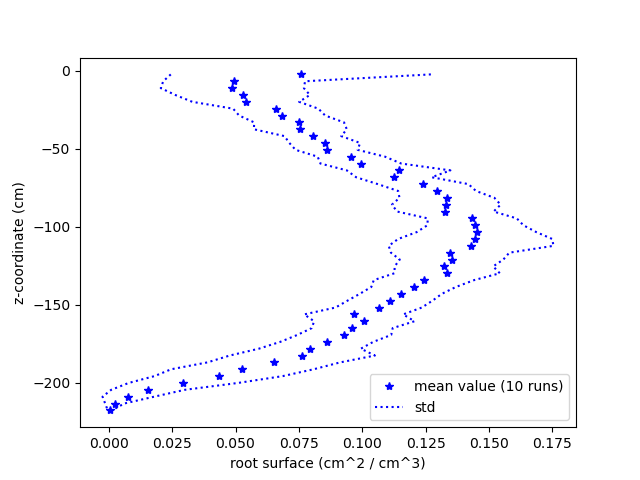
\includegraphics[width=0.7\textwidth]{figures/topics_postprocessing.png} 
\caption{Root surface densitiy versus depth including standard deviation (based on 10 simulation runs) } \label{fig:topics_postprocessing}
\end{figure}




\subsubsection*{Analysis of segment within a cropping geometry}

The following script demonstrates some of the post processing possibilities by setting up a virtual soil core experiment (see Figure \ref{fig:soilcoreGeom}), where we analyse the content of two soil cores located at different positions.

\lstinputlisting[language=Python, caption= A virtual soil core experiment (topics\_postprocessing2)]{examples/topics_postprocessing2.py}

\begin{itemize}
\item[11-15] Performs the simulation.
\item[17-22] We define two soil cores, one in the center of the root and one 10 cm translated. In L22 we pick which one we use for the further analysis. Figure \ref{fig:soilcoreGeom} shows the resulting geometry, with a soil core radius of 10 cm.
\item[24-28] Prepares three sub-figures. 
\item[31-41] Creates a root length distribution versus depth at different ages. L33 creates the SegmentAnalyser object, and L34 crops it to a fixed domain or maps it into a periodic domain. In L38 the filter function keeps only the segments, where the parameter (first argument) is in the range between second and third argument. L39 creates the distribution. 
\item[44-54] We repeat the procedure, but we crop to the soil core selected in L22. 
\item[57-89] In the third sub plot we make densities of specific root types like basal roots, first order roots, and second order roots. In L58 we crop the segments to the soil core geometry. In L63 we filter for the selected sub type, and in L64 we create the density distribution.
\item[71-73] Show and save resulting Figure \ref{fig:central} and \ref{fig:shifted} for the two soil cores (chosen in L22).
\end{itemize}

% \begin{figure}
% \centering
% 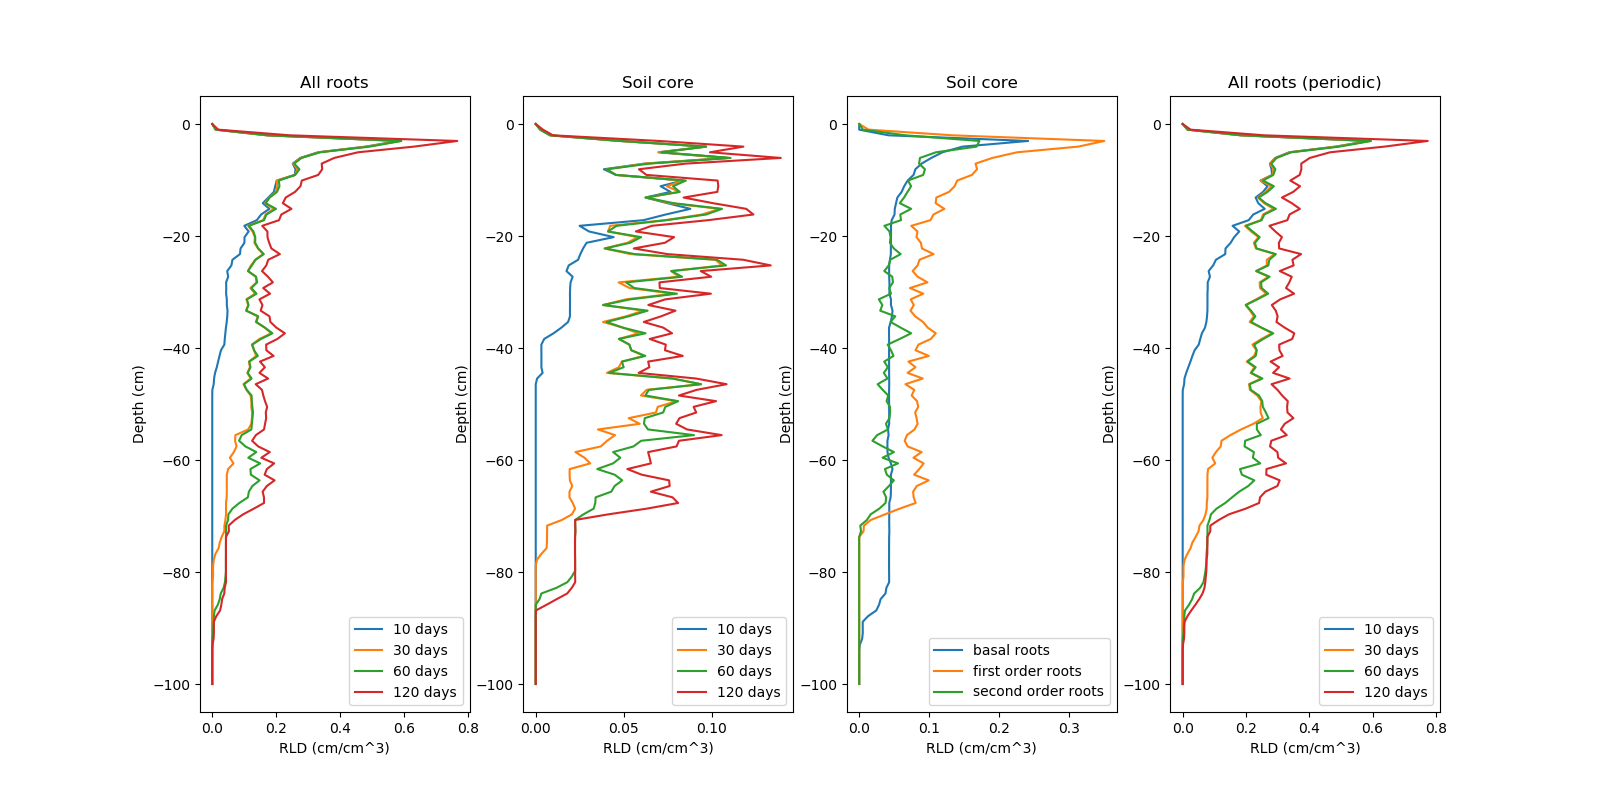
\includegraphics[width=0.7\textwidth]{example_3d.png} % 
% \caption{Virtual soil cores experiment (Example 3b): Central core (blue), shifted core (red)} \label{fig:soilcoreGeom}
% \end{figure} 


The example shows differences between the central core and shifted core (see Figure \ref{fig:central} and \ref{fig:shifted}) because the central core captures all roots emerging from the seed. The basic idea is that such analysis can help to increase the understanding of variations in experimental observations.
% 
% \begin{figure}
% \centering
% 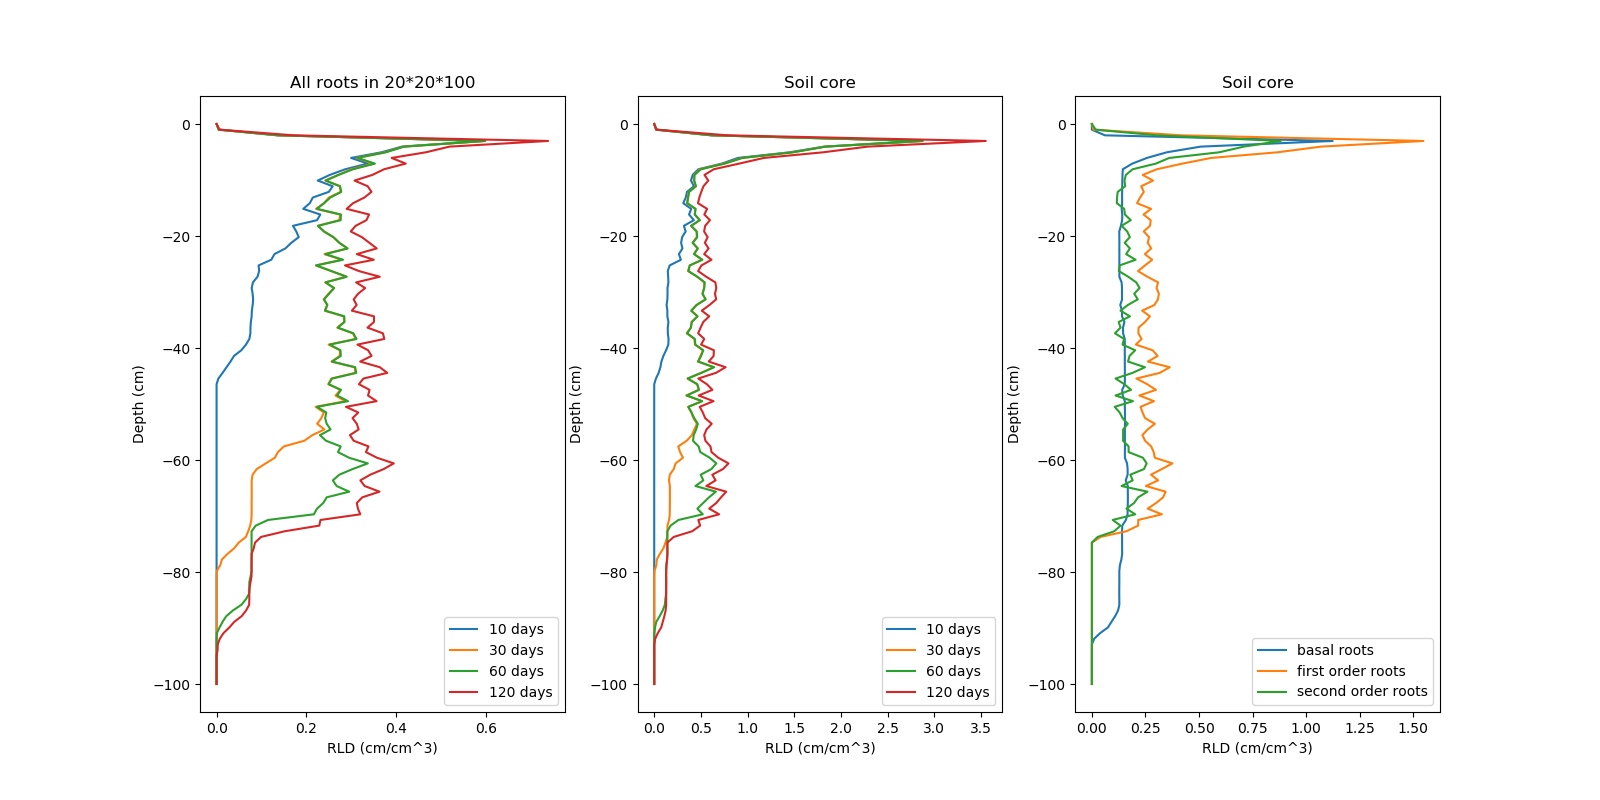
\includegraphics[width=0.9\textwidth]{example3b.png} 
% \caption{Central core (Example 3b)} \label{fig:central}
% \end{figure}
% 
% \begin{figure}
% \centering
% 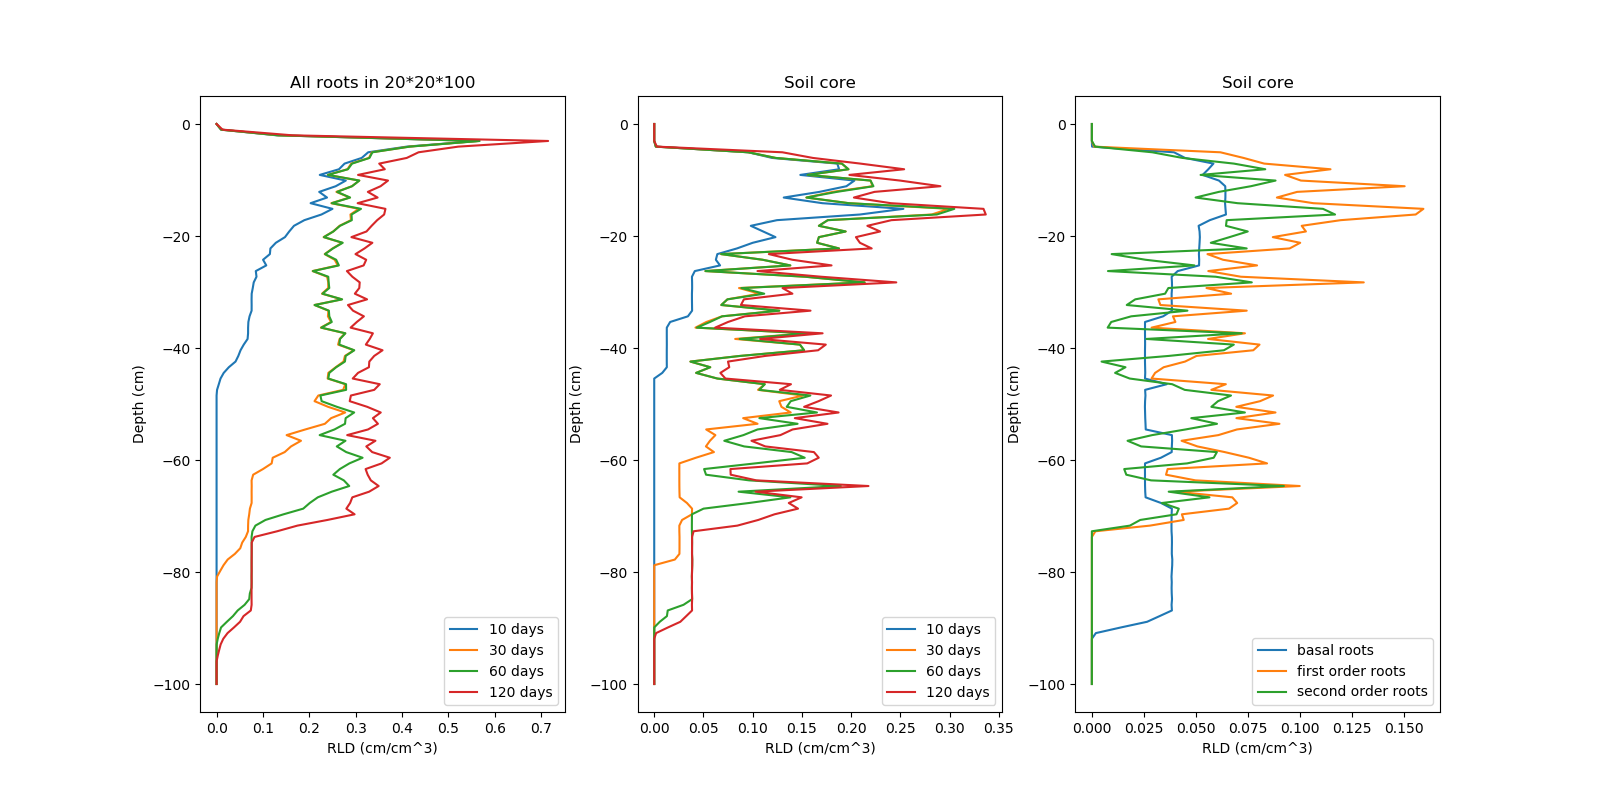
\includegraphics[width=0.9\textwidth]{example3b2.png} 
% \caption{Shifted core (Example 3b)} \label{fig:shifted}
% \end{figure}


\subsubsection*{SegmentAnalyser for measurements}

It is also possible to make use of the SegmentAnalyser class without any other CPlantBox classes (e.g. for writing vtp from measurements). The following example shows how to construct the class with arbitrary nodes and segments (e.g. from measurements). 

\lstinputlisting[language=Python, caption=SegmentAnalyser can be used on measured data (topics\_postprocessing3.py) ]{examples/topics_postprocessing3.py}

\begin{itemize}
 \item[7-11] Define some segments with data
 \item[14,15] We convert the Python list to lists of C++ types
 \item[18] We create the SegmentAnalyser object without an underlying plant
 \item[19,20] Use the Analyser object, by printing information, or writing a vtp. 
 \item[21] Visualize your results
\end{itemize}


\subsection{Visualisation} \label{ssec:visualisation}

\subsubsection*{Quick visualizations from Python}

It is possible to quickly visualize resulting geometry from Python using the module $vtk\_plot$, which offers auxilliary functions using VTK (\href{https://vtk.org/vtk-users-guide/}{VTK User's Guide}). Use 
\begin{lstlisting}[language=Python]
import visualisation.vtk_plot as vp
\end{lstlisting}
to import the module and name it $vp$.

After creation and simulaton of the plant, there are different ways to start an interactive plot
\begin{lstlisting}[language=Python]
vp.plot_segments(plant, "subType") # Option 1
ana = pb.SegmentAnalyser(plant)
vp.plot_segments(ana, "subType") # Option 2
vp.plot_plant(plant, "subType") # Option 3
\end{lstlisting}
The interactive plot can be to rotated (left mouse button), panned (mid mouse buttorn, joystick like from plot center) or zoomed (right mouse button). Per default 'creationTime', 'age', 'radius', 'subType' or 'organType' can be viusalized. But generally all parameters that will be presented in Section \ref{sec:cplantobx} can be visualized. You can save a screenshot as png file by pressing 'g', or reset view 'r', or change view by pressing 'x', 'y', 'z', and 'v'.

Option 1 and 2 are identical and can be used on Plan or SegmentAnalyser class. It visualizes the centerlines or polylines of all plant organ. A tube geometry is created around each segment. In this way it is possible to map a parameter to a colour at segment level. 
Option 3 does the plot the same way as 1 and 2, but additonally plots the leafs a polygons. The first argument is the plant or SegmentAnalyser object, the second the parameter that shall be visualized. Common choices are subType, organType, or creatiionTime, but in principle all model parameters that are presented in section \ref{sec:cplantobx} can be visualized. \\

It is possible to add arbitrary parameters using the SegmentAnalyser class: 
\begin{lstlisting}[language=Python]
ana.addData(name, data) 
\end{lstlisting}
where name is the parameter name, and data given per segment and has the length as there are segments or nodes within the SegmentAnalyser object.

If you use a functional strucural model, SegmentAnalyser offer auxilliary functions to add root hydraulic parameters:
\begin{lstlisting}[language=Python]
addAge(simtime) 
addConductivities(xylem, simtime,kr_max = 1.e6, kx_max = 1.e6)
addFluxes(xylem, rx, sx, simTime)
addCellIds(const MappedSegments& plant); // 
\end{lstlisting}
Line 1 creates segment age from the segment parameter $creationTime$ for the final simualtion time simtime. Line 2 uses a $XylemFlux$ object to evaluate the age dependent hydraulic conductivities, and optionally offers maximal values (for visualisation). It will create two parameters named $kr$ and $kx$.  Line 3 adds radial and axial fluxes named  $axial\_flux$, $radial\_flux$ based on th xylem potentials $rx$, and soil potentials $sx$ (both either matric potentials, or total potentials). Line 4 uses a $MappedSegments$ object to create cell indices named $cell\_id per$ root segment. 


\subsubsection*{How to export plant geometry for later visualization} \label{ssec:export}

There are various ways to export plant geometry for later visualization, or to use the geometry as mesh for other simulation software.

The Plant class provides outputs in RSML \citep{lobet2015root}, VTP (\href{https://vtk.org/vtk-users-guide/}{VTK User's Guide}), and for paraview python scripts for the soil container geometry. Each organ is represented as a polyline with additional data given for each organ/polyline.

\begin{lstlisting}[language=Python]
plant.write("myfile.rsml")
plant.write("myfile.vtp")
plant.write("myfile.py")
\end{lstlisting}

The SegmentAnalyser class provides outputs in VTP (\href{https://docs.paraview.org/en/latest/ReferenceManual/index.html}{ParaView documentation}), DGF (\href{https://dune-project.org/doxygen/2.4.1/group__DuneGridFormatParser.html}{Dune Grid Format} ), and text files. The Plant organs are represented by their segments.
\begin{lstlisting}[language=Python]
ana = pb.SegmentAnalyser(plant)
ana.write("myfile.vtp")
ana.write("myfile.dgf")
\end{lstlisting}


The interactive plotting tools are based on VTK and it is easy to write the resulting geometries as VTP in a binary format resulting in smaller file size. The organs are represented as polylines, the
\begin{lstlisting}[language=Python]
vp.write_plant(plant)
\end{lstlisting}
TODO there are file formats supported, e.g. mesh


The class PlantVisualizer can ...




\subsubsection*{Paraview}

how to run the macros... and render the geometry


\subsubsection*{How to make an animation} \label{ssec:animation}

In order to create an animation in Paraview we have to consider some details. There are two approaches: One is to make one vtp file per animation frame (whih will need a lot of disc space). The second approach is to export the result file as segments using the class SegmentAnalyser. A specific frame is then obtained by thresholding within Paraview using the segments creation times. In this way we have to only export one vtp file. The advantage of the first approach is, that we can also visualize plant leafs, if this is not necessary the second approach is recommended. \\






We modify example1b.py to demonstrate how to create an animation.

\lstinputlisting[language=Python, caption=Example 4c (modified from Example 1b)]{examples/example3e_animation.py} 

\begin{itemize}

\item[11,12] Its important to use a small resolution in order to obtain a smooth animation. L18 set the axial resolution to 0.1 cm. 

\item[19,29] Instead of saving the root system as polylines, we use the SegmentAnalyser to save the root system as segments.

\item[22,23] It is also possible to make the root system periodic in the visualization in $x$ and $y$ direction to mimic field conditions.

\item[26-28] We save the geometry as Python script for the visualization in ParaView.

\end{itemize}

After running the script we perform the following operations Paraview to create the animation:
\begin{enumerate}
 \item Open the .vtp file in ParaView (File$\rightarrow$Open...), and open tutorial/examples/python/results/example\_3e.vtp.
 \item Optionally, create a tube plot with the help of the script tutorial/pyscript/rsTubePlot.py (Tools$\rightarrow$Python Shell, press 'Run script').
 \item Run the script tutorial/pyscript/rsAnimate.py (Tools$\rightarrow$Python Shell, press 'Run script'). The script creates the threshold filter and the animation. 
 \item Optionally, visualize the domain boundaries by running the script tutorial/examples/python/results/example\_4e.py (Tools$\rightarrow$Python Shell, press 'Run script'). Run after the animation script (otherwise it does not work).  
 \item Use File$\rightarrow$Save Animation... to render and save the animation. Pick quality ($<$100 \%), and the frame rate in order to achieve an appropriate video length, e.g. 300 frames with 50 fps equals 6 seconds. The resulting files might be uncompressed and are very big. The file needs compression, for Linux e.g. ffmpeg -i in.avi -vcodec libx264 -b 4000k -an out.avi, produces high quality and tiny files, and it plays with VLC.
\end{enumerate}



\subsection{Playing with parameters} \label{ssec:parameters}
\subsubsection*{Initialize plant parameters from scratch} 
 
In the previous examples we opened the plant parameters from an XML file. In the following example we demonstrate how to construct a plant with a Python script without the need of any parameter file. This is especially important, if we want to modify parameters in our scripts (e.g. like it is needed for a sensitivity analysis, see Section \ref{ssec:sa}). \\

In order to set up a simulation by hand, we have to define all relevant model parameters. This is done by creating a $RootRandomParameter$, a $StemRandomParameter$, and a $LeafRandomParameter$ object for each organ order or organ sub-type, and a single $SeedRandomParameter$ for each plant type. In this section we will show how to create parameter sets, modify parameters and write XML plant parameter files. In Section \ref{sec:cplantobx} we present a detailed model description including all organ parameters. \\

Note that during the simulation, the parameters for a specific organ (i.e. OrganSpecificParamter with the specialisations RootSpecificParameter, StemSpecificParameter, and LeafSpecificParameter) are generated from the OrganRandomParameter class (with the specialisations RootRandomParameter, StemRandomParameter, and LeafRandomParameter) which represents the random distributions of certain parameters. First, we show how to construct instances of these classes, and show their parameters:
\lstinputlisting[language=Python, caption= How to create random parameter sets (specialisations of OrganRandomParameter) (topics\_parameters.py)]{examples/topics_parameters.py}
\begin{itemize}
\item[8-12] ljlkjlkjlkjlkj
\item[14-20]
\item[22-25] 
\end{itemize}



\lstinputlisting[language=Python, caption= A root system from scratch (topics\_parameters2.py)]{examples/topics_parameters2.py}

\begin{itemize}
\item[5] Matplotlib is Python's easy way to create figures like in Matlab.\item[6] NumPy is Python's scientific computing package.
\item[9,10] Create the root type parameters of type 1 and type 2.
\item[12-38] We set up a simple root system by hand. First we define the tap root L12-L26, then the laterals L28-L38. By default all standard deviations are 0. Most parameters standard deviations can be set with an additional 's' appended to the parameter name, e.g. $lmaxs$ is the standard deviation of $lmax$, see L32
\item[40,41] Set the root type parameters.
\item[43-47] Create an object of class SeedRandomParameter which defines when basal and shoot borne roots emerge. In this example we neglect basal and shoot borne roots, and just define the seed location, and deactivate basal roots by setting their maximal number $maxB$ to 0 ($firstB$ and $delayB$ are ignored in that case). 
\item[48] Sets the root system parameters.
\item[53] We choose the simulation times in a way that we can see the temporal development, and that all lateral roots have emerged in the final time step.
\item[54-70] Within the simulation loop we create Figure \ref{fig:ip}. L58-61 defines the limits and titles. In L63 we retrieve the roots as polylines which are represented by a list of nodes. In L64-67 we plot the $x$ and $z$ coordinates for each segment ($n$, $n2$) as green line. 
\item[75-80] It is not only possible to set all model parameter, 
but to retrieve the parameters after the simulation with rs.getParameter(), which returns one value per root. For all parameters that are derived from a random distribution the root specific parameter is returned (e.g. $la$, L78), i.e. the values that were drawn from the normal distribution. The root random parameter can be accessed by adding '\_mean', '\_dev' to the parameter value (e.g. $la\_mean$, L79).
\end{itemize}

Note that all parameters can be set and modified within Python. Especially, standard deviations can be set to zero in order to be able to precisely predict the result. For example we can calculate the total root system length analytically, and check if the numerical simulation yield the (exact) same result. This is performed in the tests test\_root.py, and test\_rootsystem, which is used to test and validate CPlantBox (see folder CPlantBox/test).

With such simple simulations, we can quickly check if the model does, what we expect. For example the maximal number of laterals of above parameters is 16 
$= round(lmax - la - lb)/l_n +  1$. We can calculate the time when the final lateral emerges as $-(lmax/r)*\ln(1-(lmax-l_n/2)/lmax)$ = 122.8 days. At simulation time 125 the last lateral root that has emerged is 2.2 days old, and therefore approximately 4.4 cm long (initial growth rate $r_1 = 2$), which agrees with Figure \ref{fig:ip}.

By default the length of the apical zone is fixed, when the root is created. During growth the apical zone stays in the interval $[la - l_n/2, la+l_n/2]$. The first branch emerges at length $lb$, when the root length reaches $lb +la$.

In the following two subsections we show, how tropism parameters and inter lateral spacing will affect the resulting root system.

% \begin{figure}
% \centering
% \includegraphics[width=\textwidth]{figures/topics_parameters2.png}
% \caption{Root development} \label{fig:ip}
% \end{figure}

\subsubsection*{Modify inter-lateral spacing (ln, lnk)} 

A single root is divided in basal zone, root branching zone, and root apical zone. Basal and apical zone are given by the parameters $la$, and $lb$ with standard deviations $la_s$ and $lb_s$. The branching zone has the size $lmax-la-lb$, where $lmax$ is the maximal root length. The branching zone is divided into inter lateral distances $l_n$, which are values drawn from a normal distribution with standard deviation $l_{ns}$. All values are fixed when the root is created This is performed in the method RootRandomParameter::realize(). The chosen parameters reflect the root growth under perfect conditions. Based on this, the root development can then be influenced by environmental conditions e.g. impeding growth speed, or lateral emergence, see Section \ref{sec:functional}.

Normally, the setting constant branching distances is sufficient, but sometime experimental data indicate that inter lateral distances are smaller, or larger near the base than near the root tip. The reason for this could be soil root interaction (e.g. root response to dense or nutritious layer), or within the genotype. We added a purely descriptive parameter to mimic such experimental observations. The parameter $lnk$, which is zero per default, defines the slope, at the mid of the branching, altering the inter lateral distance linearly along the root axis. In the following script, we demonstrate the usage of $lnk$.

\lstinputlisting[language=Python, caption=Example 2c (topics\_parameters2.py)]{examples/topics_parameters2.py}

\begin{itemize}
\item[10-13] A root system with a single tap root is created. 
\item[16,16] The axial resolution, and insertion angle is defined. We take a very large axial resolution for the tap root, since we visualize the nodes later on, and we want to see only lateral branching nodes.
\item[18-24] Definition of the tap root. Standard deviations are zero, we do not want any variations. Tropism parameters are chosen in a way, that the tap root grows straight downwards.
\item[26-29] Definition of the first order lateral. Tropism is a strict exotropism (i.e. root follows its initial growth direction).
\item[31,32] The parameter values we want to visualize.
\item[36] Resets the root system (to $simTime = 0$). Root parameters are not changed. 
\item[38,39] Sets the values for this subplot. 
\item[41,42] Runs the simulation
\item[44-56] Creates the subplots. First (L47-49) we plot all segments in green. And second (L51-53) we plot all nodes of the tap root as red asterisks.
\item[58-60] Creates Figure \ref{fig:spacing}
\end{itemize}

The mid column of Figure \ref{fig:spacing} shows to different inter lateral distances, 4 (top) and 2 (cm) bot. The left column demonstrate the use of negative values for $lnk$ which results in larger distances near the base. The right column has positive values for $lnk$, which will result in smaller distances near the base. The $i$-th inter distance is calculated as $ln_i = ln + lnk (x_i-mid_x)$, where $x_i$ is the position within the branching zone, and $mid_x$ is the mid of the branching zone. This is done in RootRandomParameter::realize(). Note that $lnk$ is dimensionless and the slope in the linear equation. At mid of the branching zone the inter-lateral distance equals $ln$. 

% \begin{figure}
% \centering
% 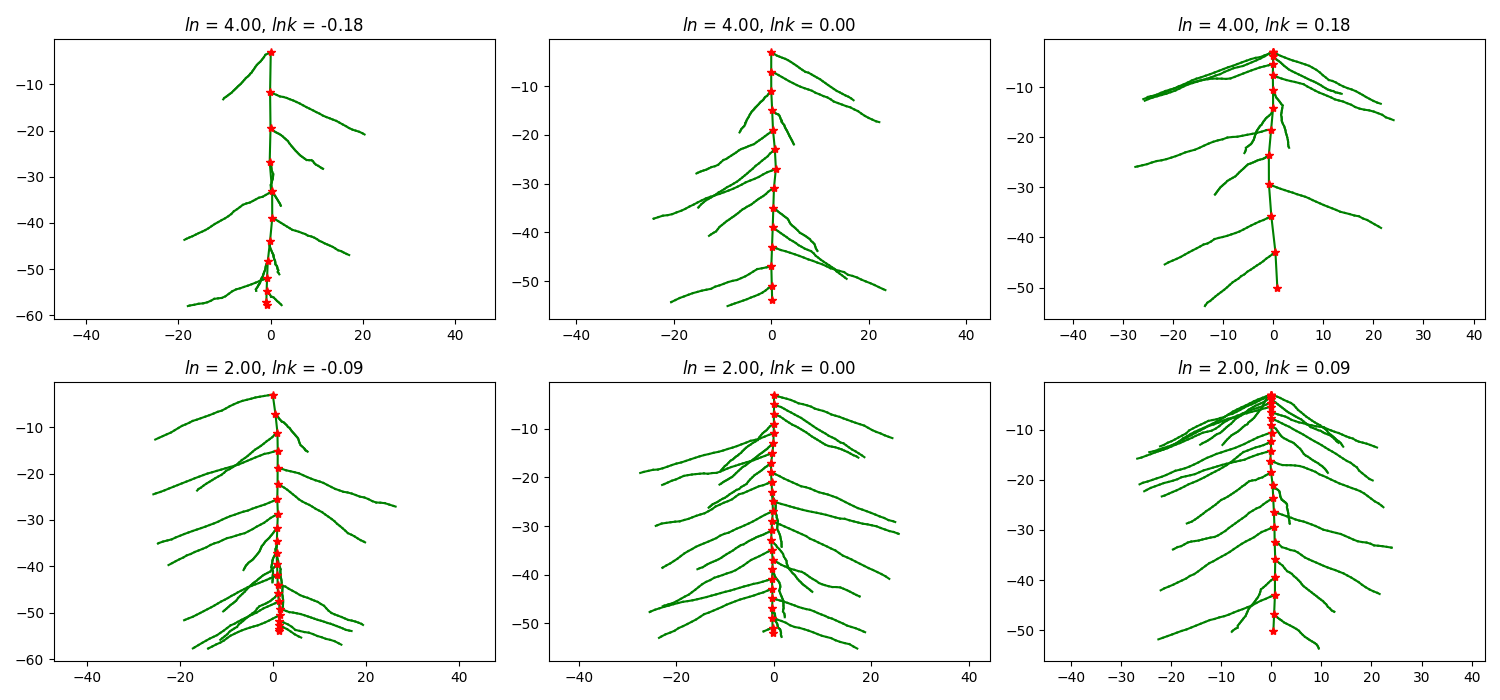
\includegraphics[width=0.99\textwidth]{fig_lateralspacing.png}
% \caption{Inter-lateral spacing, larger near base (left column), constant (mid column), and smaller near base (right column) } \label{fig:spacing}
% \end{figure}

In the following we show, how to analyse model results on a per root basis using the RootSystem class. To create density distributions the resulting root segments are analysed using the SegmentAnalyser class, described in Section \ref{sec:sa}.


\lstinputlisting[language=Python, caption=Example 2c (topics\_parameters3.py)]{examples/topics_parameters3.py}





\subsection{Plant tropism} \label{ssec:tropism}
The change in root growth direction is described by tropisms. In the following we show how to implement directed growth, and demonstrate how to simply make new user defined tropism rules. 


\subsubsection*{Root tropism parameters $N$ and $\sigma$} 

We show the influence of the parameters $N$ and $\sigma$ in the case of gravitropism. The parameter $N$ [1] denotes the strength of the tropism, and $\sigma$ [cm$^{-1}$] the flexibility of the root, i.e. the expected angular variation per cm root length. 

\lstinputlisting[language=Python, caption=Example 2b (topics\_tropism.py)]{examples/topics_tropism.py}

\begin{itemize}
\item[10-13] We choose the parameter values $N$ and $\sigma$ we want to plot. It might be interesting to change the initial insertion $angle$, and the axial resolution $dx$. Note that a change in axial resolution should not qualitatively change the resulting images.

\item[15-18] The root system is created and SeedRandomParameters are set to produce a basal root every third day. 

\item[20-23] The RootRandomParameter for tap and basal roots is defined.

\item[25-28] The loop runs over the parameters we want to modify. We create a subplot for each configuration, and start with a new root system by calling reset in L28.

\item[30-34] We set the parameters (L30,L31) and do the simulation (L33,L34)

\item[36-44] Matplotlib is used for visualization (looping over the segments is rather slow). L36 gives a list of all nodes, and L37 of all segments as two node indices. Therefore, each segment starts at node n1 and ends at node n2, as defined in L39.

\item[L48] Creates Figure \ref{fig:tropism}.
\end{itemize}

In the first column ($\sigma$=0) of Figure \ref{fig:tropism} nothing happens, because if the root has no flexibility to bend, the strength has no influence on the resulting root system. The first row ($N$=0) shows the influence of $\sigma$ only. The growth is undirected, because the strength of the gravitropism is zero. If the roots have small flexibility, they grow downwards because they initially do. 

The other subplots show different shapes of the root system. We normally derive the two parameters $N$ and $\sigma$ by visual comparison. Note that results are independent of the root axial resolution $dx$ and the temporal resolution.
% 
% \begin{figure}
% \centering
% 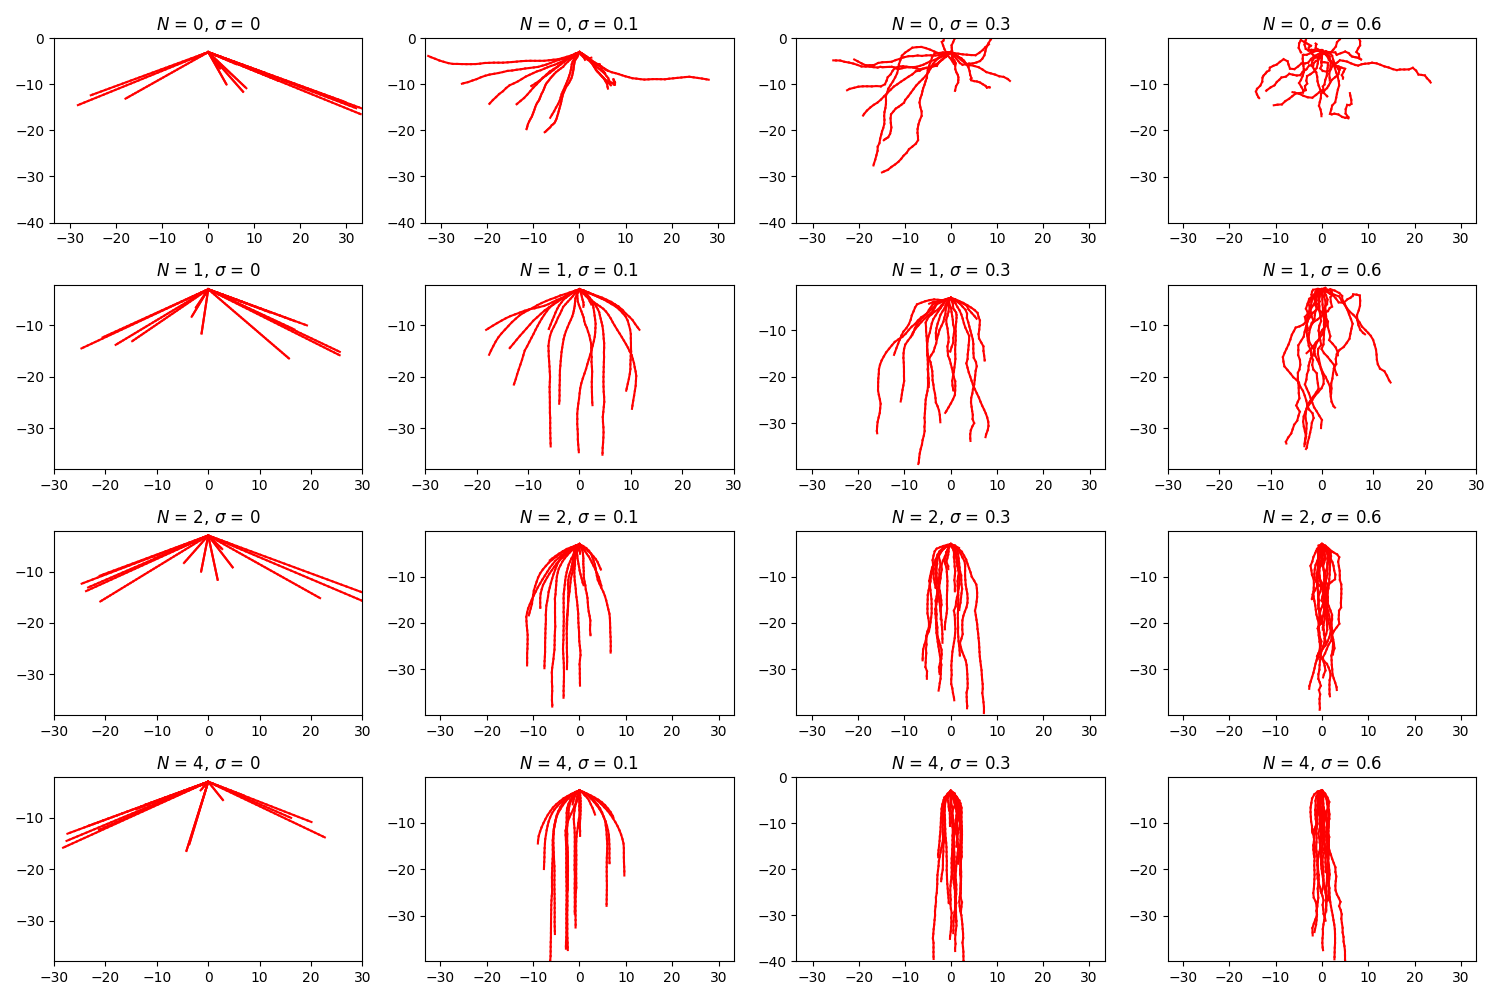
\includegraphics[width=\textwidth]{fig_gravitropism.png}
% \caption{Influence of $N$ and $\sigma$ in case of gravitropism} \label{fig:tropism}
% \end{figure}



\subsubsection*{Hydro- and chemotropism} 


Root growth direction is influenced by soil conditions such as water content, soil strength, or nutrient concentration. In the following example we model the influence of a nutrient rich layer to root system development

\lstinputlisting[language=Python, caption=Example 4a]{examples/example4a_hydrotropism.py}

\begin{itemize}

\item[6-9] Creates the root system and opens the parameter file

\item[12-17] Change the tropism for all root types: L13 modifies the axial resolution, L14 set the tropism to hydrotropism, and L15-16 sets the two tropism parameters. The parameter $\sigma$ is set to 0.4 for the tap root ($subType$ = 1), and to 1. for the rest of the root types.

\item[19-25] Definition of a static soil property using SDF. We first define the geometry (L20-L21), and then create a static soil (L22) that obtains the maximal value $maxS$ inside the geometry, 
$minS$ outside the geometry, and linear slope with length $slope$. At the boundary the soil has the value $(maxS+minS)/2$.

\item[28] Sets the soil. Must be called before RootSystem::initialize()

\item[41] Initializes the root system, and among others sets up the hydrotropism. 

\item[33-39] Simulation loop

\item[42] Exports the root system geometry

\item[45-46] We actually do not wish to set this geometry, but we abuse the writer of the class RootSytem to export a Python script showing the layer geometry. The resulting ParaView visualization is presented in Figure \ref{fig:chemo}.

\end{itemize}

% \begin{figure}
% \centering
% 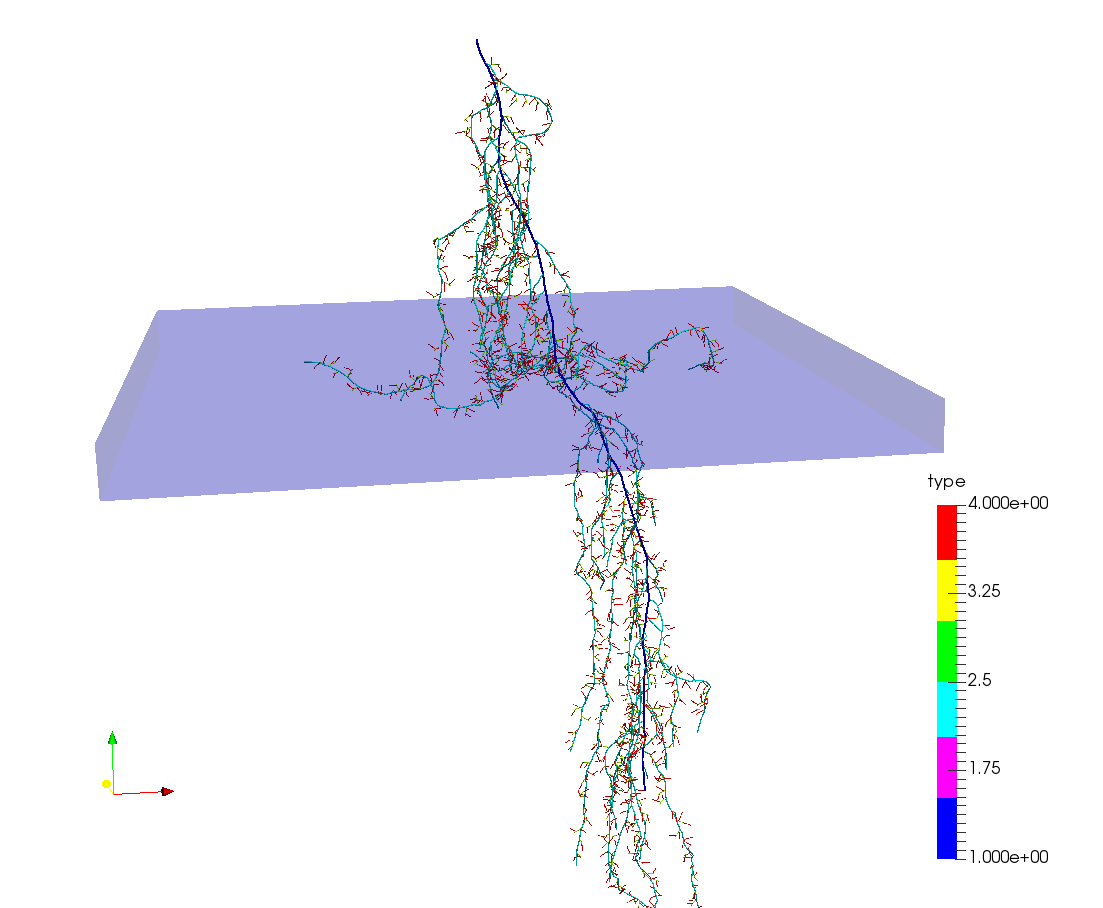
\includegraphics[width=0.7\textwidth]{example4a.png}
% \caption{Chemotropism in a nutrient rich layer (Example 4a)} \label{fig:chemo}
% \end{figure}

Normally, the simulation is created from a set of parameters. For tropisms these are the type of tropism $T$, number of trials $N$ , and tortuosity $\sigma$. There are only a few predefined tropisms called 'gravi', 'plagio', 'exo', or 'hydro', but it is simple to add user defined tropisms.
The following example demonstrates how to define a root age dependent tropism, where roots first grow according to exotropism (following the inital growth direction), and after a certain age change to gravitropic growth.

The new tropism class must be derived from the class Tropism. In CPlantBox tropism is realised with a random optimization process, where the 'best' direction is chosen from $N$ possible direction, according to an objective function that is minimized. Normally, it is sufficient to overwrite this function, called Tropism ::tropismObjective, to change the tropism behaviour. This can be done in Python or in C++. The classes Hydrotropism, Gravitropism, and Plagiotropism (in tropisms.h) are examples for this procedure.

If the whole concept of random optimization is altered, Tropism ::getUCHeading must be overwritten, which is only possible in C++. If the geometry model is also changed Tropism::getHeading must be overwritten.

The following example shows how to implement a new tropism in Python. Two new tropism are introduced:
The first does nothing but to output the incoming arguments of the method Tropism::tropismObjective to the command line (e.g. for debugging). The second one describes a root age dependent tropism that starts with exotropism and changes with root age to gravitropism.

\lstinputlisting[language=Python, caption=Example 4b]{examples/example4b_usertropism.py}

\begin{itemize}

\item[8-19] Creates a new tropism that just writes incoming arguments of Tropism ::tropismObjective to the command line. This can be used for debugging. The new class is extended from rb.Tropism, and the method Tropism ::tropismObjective is overwritten with the right number of arguments.

\item[22-37] Again, we extend the new class from rb.Tropism. In L25-30 we define our own constructor. Doing this two things are important: (a) the constructor of the super class must be called (L26), and (b) the tropism parameters $n$, and $\sigma$ must be set (L29). 
Furthermore, the constructor defines two tropisms: exo- and gravitropism, that are used in Tropism::tropismObjective at a later point, and a root age that dermines when to switch betwee exo- and gravitropism. \\
In L32-L37 the method Tropism::tropismObjective is defined. We choose the predefined objective function depending on the root age.

\item[41-45] Sets up the simulation.

\item[48-51] L48,L49 creates the first user defined tropsim. Since we did not define a constructor Tropism::setTropismParameter must be called. L50 creates the second user defined tropism.  In L51 the tropism is chosen, using the method Tropism::setTropism. The second argument states for which root type it applies. 
Number 4 is the (default) root type for basal roots, -1 states that the tropism applies for all root types (default = -1).

\item[54-58] The simulation loop. 

\item [61] Exports the result producing Figure (\ref{fig:tropism}). 

\item [64] VTK plot.

\end{itemize}

% \begin{figure}
% \centering
% 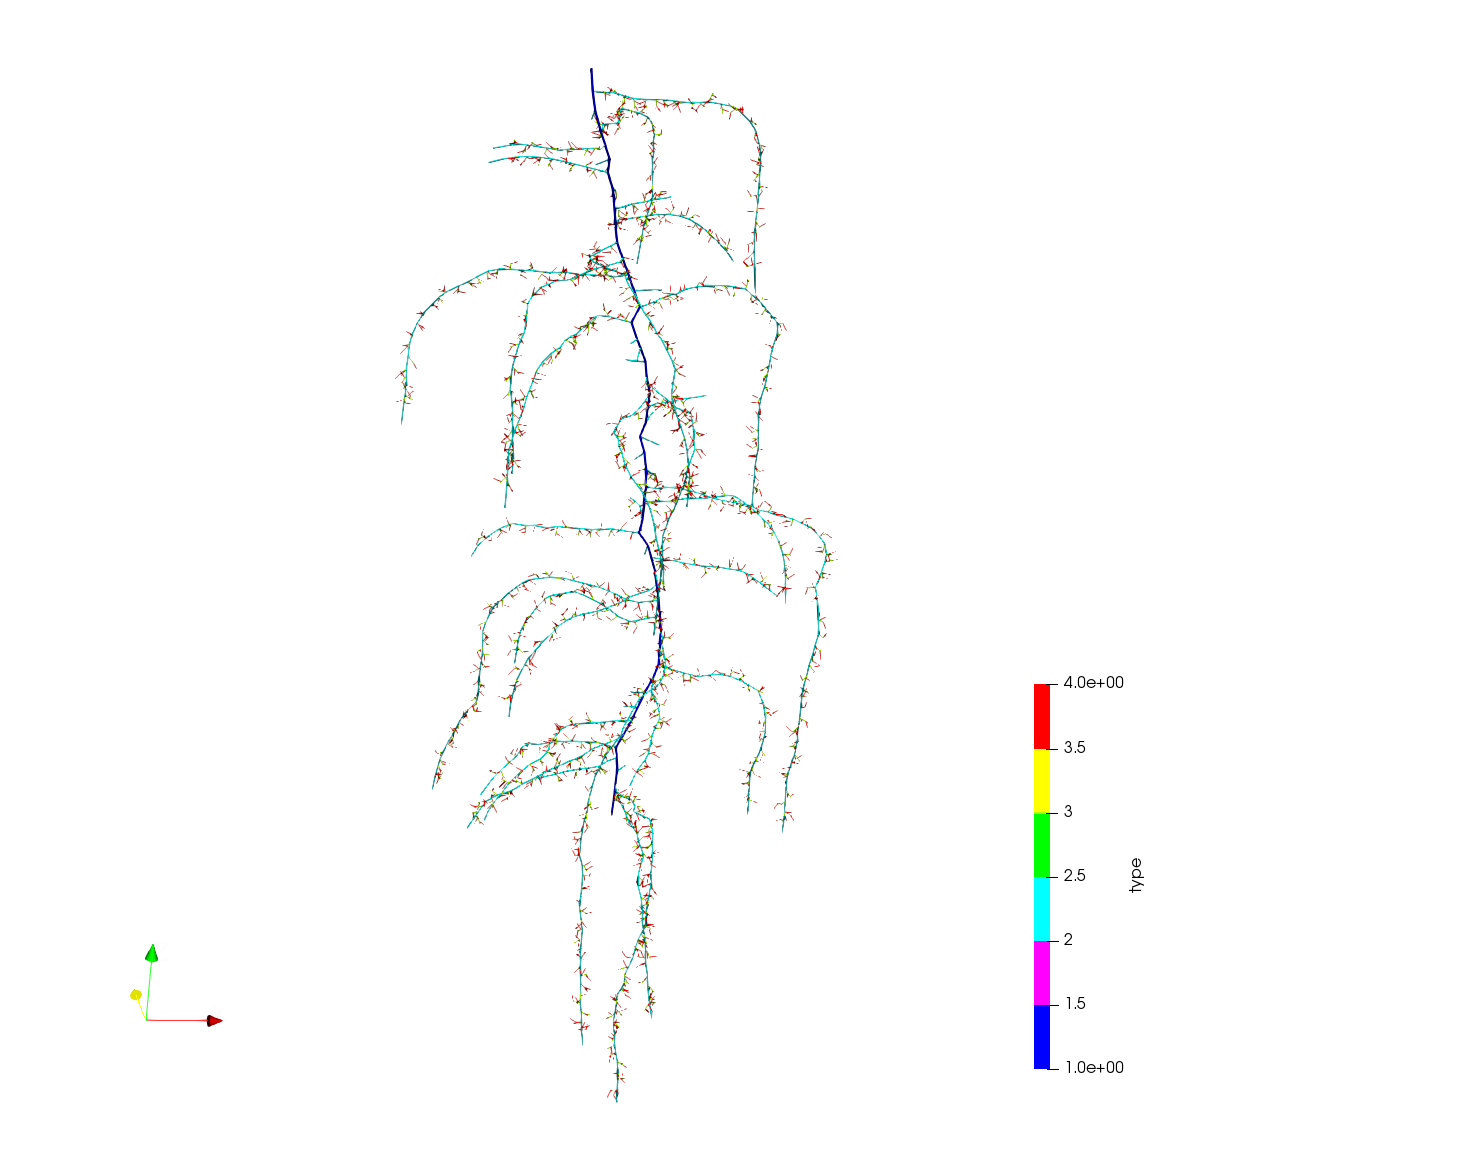
\includegraphics[width=0.7\textwidth]{example4b.png}
% \caption{Depending on root age the laterals follow plagio- or gravitropism (Example 4b)} \label{fig:tropism}
% \end{figure}


\subsection{Sensitivity analysis} \label{ssec:sa}
%
In the next part we vary given parameters in order to make a sensitivity analysis. This takes a lot of simulation runs, and we demonstrate the of use parallel computing to speed up execution.

In this exemplary sensitivity study we will vary the insertion angle of the tap and basal root, and look at the resulting change in mean root tip depth and root tip radial distance. 

\lstinputlisting[language=Python, caption=Example 2f]{examples/example2f_sensitivity.py}

\begin{itemize}

\item[12-20] Defines a function to set all standard deviations proportional to the parameter values. We use this function in the following to set the standard deviation to zero everywhere. 

\item[23-29] Parameters of the analysis. $N$ denotes the resolution of the parameter we vary, and $runs$ the number of iterations, i.e. a total of $N\cdot runs$ simulations are performed. In L29 we define the insertion angle to be varied linearly between 0 and $\pi/2$.

\item[33-52] Definition of a function that performs the simulation and returns mean root tip depth and radial distance. First we create a root system and set the standard deviation to zero L34-L36. L37, amd L39 sets the insertion angle. L41 initializes the root system and states that basal root are of root type 1 (same as tap root). The False value turns of verbosity to avoid any outputs to the console. L42 performs the simulation. L44-L51 calculates the mean root tip depth and radial distance. 

\item[55-73] This section performs the computation of all simulation runs. L55-56 preallocates the resulting arrays. L62-L68 performs the parallel computations, index $i$ is the index of the insertion angle. L71-73 calculates the mean values per simulation run.

\item[74-83] Creates the resulting Figure \ref{fig:sensitivity}. Note that the resulting curves become smoother, if the number of runs is increased (L28).

\end{itemize}

% 
% \begin{figure}
% \centering
% 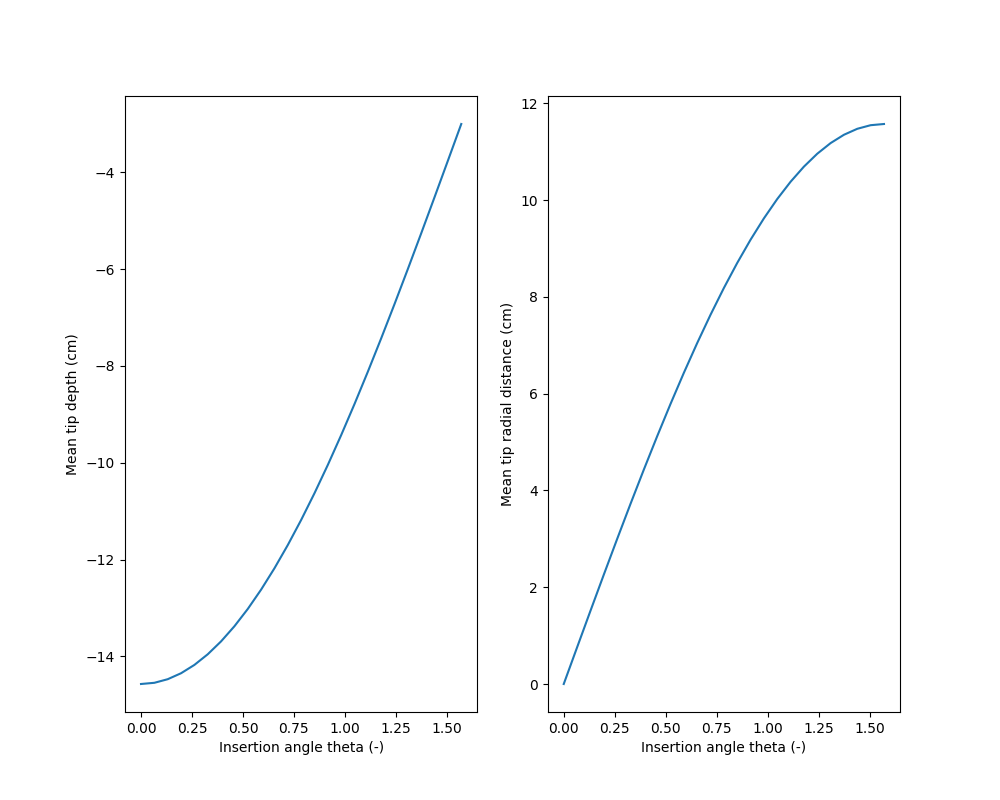
\includegraphics[width=0.7\textwidth]{example_4b.png}
% \caption{Sensitivity of mean root tip depth (left) and radial distance (right) to the insertion angle theta (Example 2f) } \label{fig:sensitivity}
% \end{figure}


\subsection{Interaction Feedback} \label{ssec:interaction}
%
Root growth is strongly influenced by pedo-climatic conditions, and plant internal state. CPlantBox offers 'build in' ways to develop such models, see \cite{schnepf2018crootbox}. 

CPlantBox is a bottom up model were root growth is first defined under perfect conditions. Adding mechanisms to take environmental conditions into account will alter the root system development by impeding root growth, and by changing soil allocation by roots due to root tropism and due to altered branching patterns.

In this section we assume static soil conditions, and demonstrate the predefined ways how the soil can affect root growth.
Dynamic soil conditions are described in the following Section \ref{s:coupling}. 

Implemented root responses are the change in direction of the growing root tip, as described in previous Section \ref{sec:tropism}.
Further root responses are 
\begin{itemize}
 \item scaling of the elongation rate 
 \item change of insertion angle
 \item change of lateral emergence probability
\end{itemize}

\subsubsection*{Scaling the elongation rate} \label{sec:elongation}

Root elongation rate is influenced by soil properties such as water content, temperature, soil density, solutes, and many more. Regarding the processes that are investigated, various models can be applied. In CPlantBox the elongation rate is scaled with no predefined interpretation, i.e. we have to define a elongation rate scaling, which is dependent on such soil properties. The following example defines two compartments (one left, one right), where we change this scaling, and then analyse the results. The same procedure will be used in Example \ref{sec:insertion_angle} and \ref{sec:branching}.

\lstinputlisting[firstline=1, language=Python, caption=Example 5a]{examples/example5a_elongation.py}

\begin{itemize}

\item[7-10] Creates the root system and opens the parameter file.

\item[13-17] We create a confining box with two overlapping boxes called $left$ and $right$. These geometries are used for later analysis.

\item[20-24] We define static soil properties using SDF (L23, L24) as we did in Section \ref{sec:hydro}. 
The left compartment has the value $minS$, the right $maxS$, between them is a linear gradient of length $slope$. 

\item[27-31] Sets the scaling functions. L29 adjusts axial resolution and L30 tortuosity $sigma$. L31 sets the scale elongation function $f_{se}$ to the soil property (i.e. scales to $minS$ in the left, $maxS$ in the right compartment). 

\item[34-39] Initialization and simulation loop. In a dynamic setting, $soilprop$ needs to be updated in each time step (comment L38).

\item[42-50] Analysis the root length in the left and right compartment. With parameters $minS$ and $slope$ only approximately $21\%$ are located in the left compartment.

\item[53, 54] Writes the results for Paraview visualization (see Figure \ref{fig:elongation}).

\item[57] A vtk simulation of root lengths. Press 'y' to obtain a x-z view of the root system to better see the effect. 

\end{itemize}
 
Next, we give a short layout, how the code would look like, if we take measured data (e.g. density versus depth), and include it in the simulation. 

\lstinputlisting[firstline=1, language=Python, caption=Example 5b]{examples/example5b_scaleelongation.py}

\begin{itemize}

\item[12-16] In L12 an EquidistantGrid1D is created, which is a specialisation from SoilLookUp (in soil.hh). It represents a 1D grid from 0 cm to -100 cm as soil with 100 layers. Additionally scalar data are attached to the grid, L13, L14 we create example soil strength data. From this data we calculate the elongation scales (L15), and set it as grid data (L16). 

\item[L17, L18] Retrieve the elongation scale data at two points. The data is given per layer, no data interpolation is performed.

\item[20, 21] Sets the elongation scaling function to all root types.

\item[25-32] Subsection \ref{ssec:animation} explains how to make an animation in Paraview. Here we use another (slower) approach to create the animation (and a preview) directly in vtk. For this we create an AnimateRoots object (L26), choose the domain size, and start the rendering (L32). 

\item[34-50] Simulation loop. If soil strength changes, the elongation scales must be calculated again (L32), and attached to the grid (L35). The frames of the animations are written in L50. While the approach is convenient, it is rather slow since for each frame a SegmentAnalyser object is created and rendered from scratch which is not feasible for large root systems. 

\item[52,53] Exports results as vtp, and creates a vtk plot. The effect of the dense layer can hardy be seen in the results (between -10 and -15 cm depth, laterals will be shorter). But the created animation reveals the effect (see exported video example5b.ogv). 

\end{itemize}

% \begin{figure}
% \centering
% 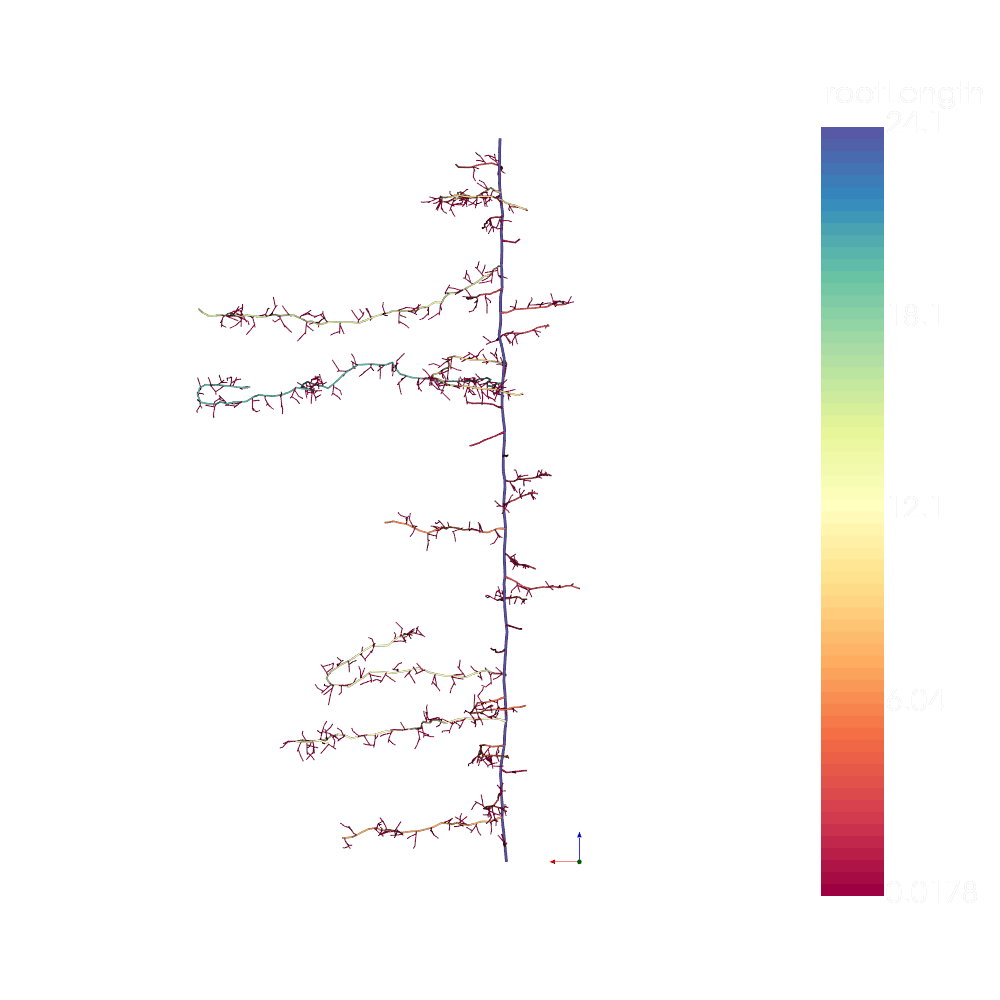
\includegraphics[width=0.5\textwidth]{example5a.png}
% \caption{Root elongation rate} \label{fig:elongation}
% \end{figure}


\subsubsection*{Change of insertion angle} \label{sec:insertion_angle}

Nutrient concentration influences the angle between parent roots and laterals. % todo ref
Analog to Example 5a two compartments are created, and the insertion angle is scaled accordingly.

\lstinputlisting[firstline=1, language=Python, caption=Example 5c]{examples/example5c_insertionangle.py}

\begin{itemize}

\item[27-32] Sets the insertion angle scaling functions to second order laterals only (L29). L20 adjusts axial resolution and, L31 tortuosity $sigma$, and L32 sets the scale insertion angle function $f_{sa}$ to the soil property. Additionally, the maximal length of second order roots is redoubled. 

\item[34-39] Initialization and simulation loop.

\item[42-50] Analysis the root insertion angle in the left and right compartment. 

\item[53, 54] Writes the results for Paraview visualization.

\item[57] A vtk simulation of root lengths. Press 'y' to obtain a x-z view of the root system to better see the effect (see Figure \ref{fig:insertion}). 

\end{itemize}

% \begin{figure}
% \centering
% 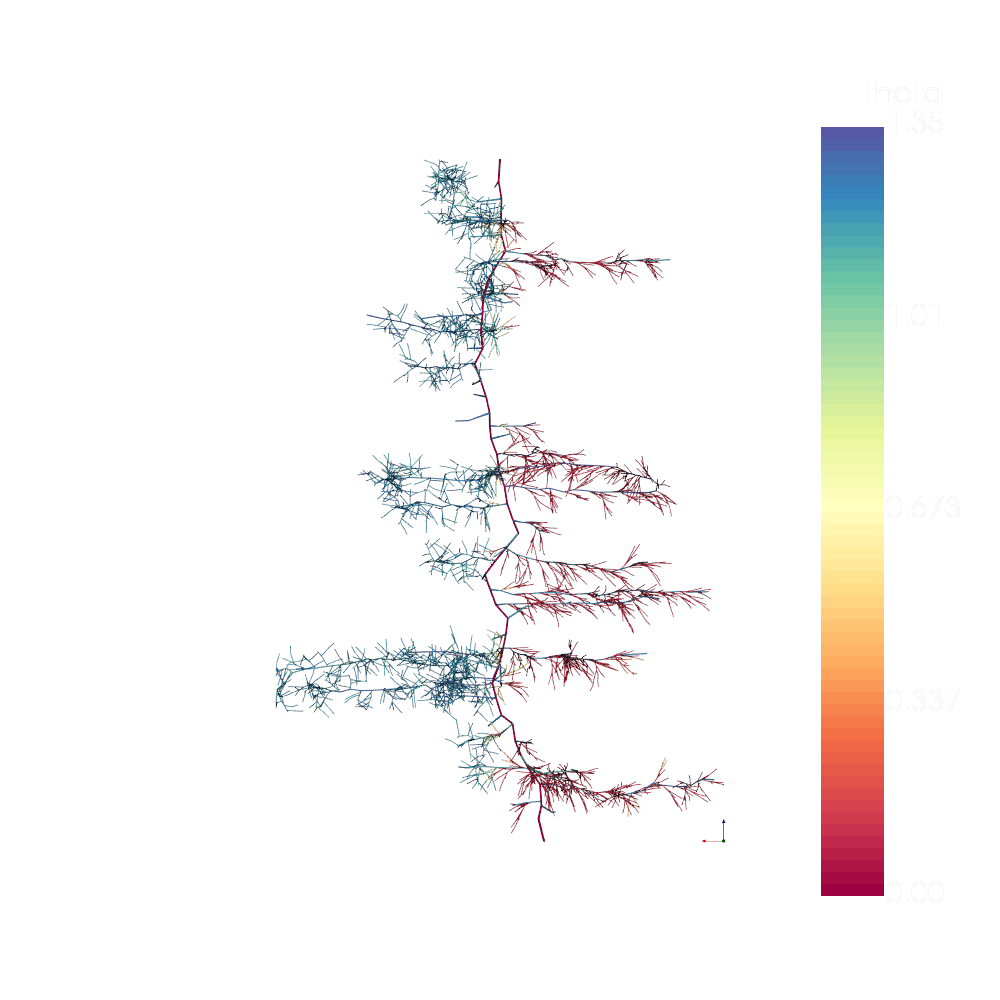
\includegraphics[width=0.5\textwidth]{example5c.png}
% \caption{Insertion angle} \label{fig:insertion}
% \end{figure}


\subsubsection*{Change of lateral emergence probability} \label{sec:branching}

Soil properties can affect branching patterns. In the following example two compartments are created ( analog to Example 5a), and the branching probability is modified in each of them.

\lstinputlisting[firstline=1, language=Python, caption=Example 5d]{examples/example5d_branching.py}

\begin{itemize}

\item[27-30] Adjusts axial resolution and tortuosity.

\item[33, 34] We adjust the inter lateral distances by making it smaller for a factor five.

\item[35, 36] We set the branching probability scaling for the second order laterals. The scaling value means the probability that the branch occurs per day, i.e. 1 means the laterals always emerge (left compartment), or that they emerge with a chance of 0.2 \% per day (right compartment). 

\item[46-54] Analysis the root insertion angle in the left and right compartment. 

\item[61] A vtk simulation of root lengths. Press 'y' to obtain a x-z view of the root system to better see the effect (see Figure \ref{fig:probability}). 

\end{itemize}

Note that a scaling of zero means, that the laterals do never emerge, one means they always do. While the branching probability model is limited, it is easy to modify it to implement plant systemic responses. For this a suitable SoilLookUP must be defined and the method getValue(x, organ) must be overwritten, implementing the plant control of the branching probabilities. 

% \begin{figure}
% \centering
% 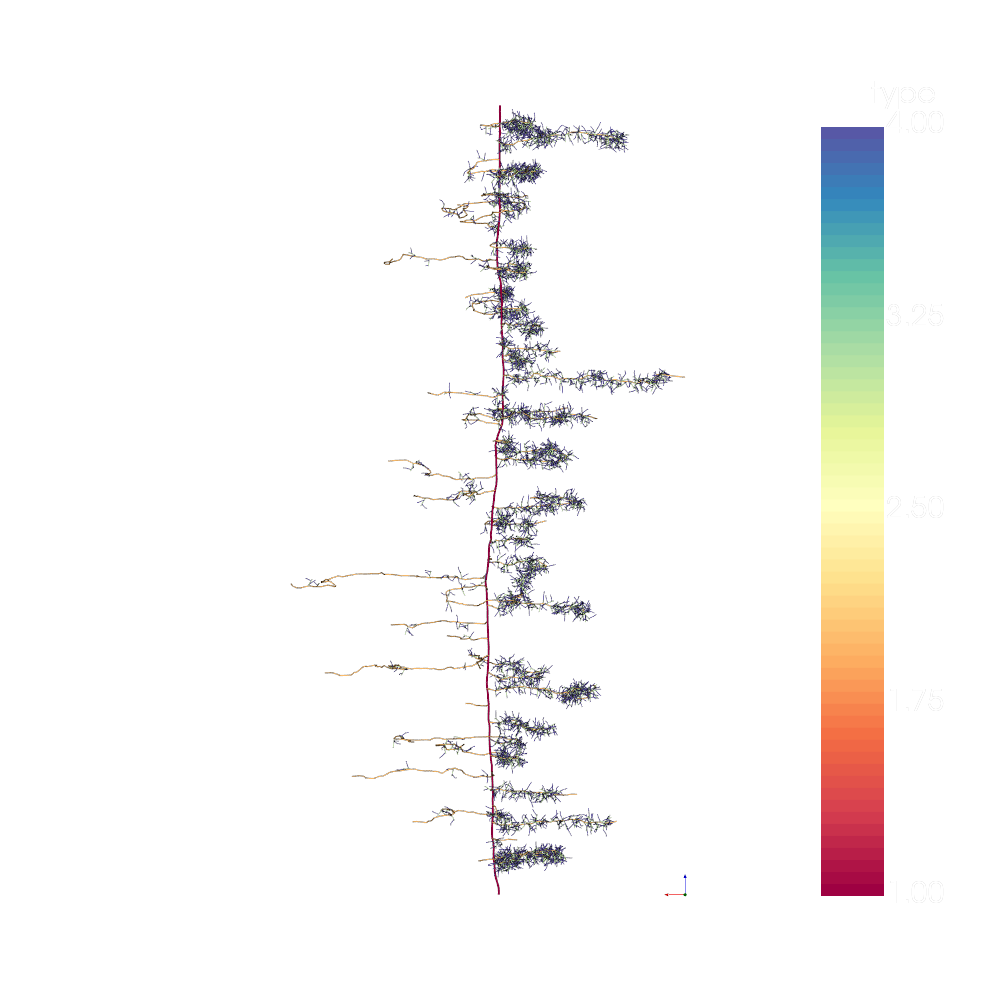
\includegraphics[width=0.5\textwidth]{example5d.png}
% \caption{Branching density (probabilistic model)} \label{fig:probability}
% \end{figure}


\subsection{RSML} \label{ssec:rsml}
%






\newpage
\section{CPlantbox Structural Model} \label{sec:cplantobx}

In this section we describe the underlying strutural model of CPlantBox including all model parameters.

\subsection{General plant organs} \label{ssec:organs}




\subsection{Seed} \label{ssec:seed}




\subsection{Stem} \label{ssec:stem}




\subsection{Leaf} \label{ssec:leaf}




\subsection{Root} \label{ssec:root}







\newpage
\section{Plant Structural Functional Models} \label{sec:fspm}

\subsection{Plant hydraulics} \label{ssec:hydraulics}
% \subsubsection*{Water movement within the roots} \label{sssec:xylem}

Since water movement within the roots is often needed, it is implemented directly in CPlantBox (in the class XylemFlux) following \cite{meunier2017hybrid}. However, usage is optional, and any other transport code can be used (e.g. if solutes are considered). XylemFlux sets up the linear system, and the sparse linear system is then solved in Python using scipy (using the class XylemFluxPython defined in xylem$\_$flux.py).

The following example is based on benchmark M3.1 \citep{schnepf2019call} with constant conductivities, but not with a given root system, but a simulated one.

\lstinputlisting[firstline=1, language=Python, caption=Example 6b]{examples/example6b_xylemflux.py}
\begin{itemize}

\item[11-15] All parameters that will be used later on.

\item[18-23] The root system (similar to last section). 

\item[26-31] The MappedRootSystem is wrapped with the XylemFluxPython class, which extends the XylemFlux class, which computes the xylem matric flux potential. L27, L28 sets the radial and axial conductivity. L29 retrieves the root system nodes for later visualisation. The pressure surrounding the the root system is either defined as pressure surrounding each root segment, or as soil cells, in which the root segments are located. L30, L31 sets a soil containing of one single cell with index 0. 

\item[34-36] XylemFluxPython defines solvers like solve$\_$dirichlet for Dirichlet boundary condition (predefined collar matric potential), solve$\_$neumann for Neumann boundary condition (predefined collar flux), and solve which switches between Dirichlet and Neumann at some critical pressure (the plant wilting point).
The arguments of solve$\_$dirichlet are the simulation time (to calculate age dependent conductivities), the root collar pressure head, the pressure around the root collar, the soil matric potential around the root segments or per soil cell, and a boolean value that decides if the potentials are given per soil cell (True) or per segments (False). The return value $rx$ contains the xylem matric potentials per segment. L35 calculates the fluxes into the soil (negative values mean into the root). The bool argument determines if we approximate the flux, or use the exact solution by \cite{meunier2017hybrid}.
L36 determines the root collar flux.

\item[39-43] Plots the results.

\item[46-49] Creates the VTK plot, adding the soil matric potentials and fluxes. L49 picks either $rx$ or $fluxes$ for vizualisation, see Figure \ref{fig:xylemfluxa} and \ref{fig:xylemfluxb}.

\end{itemize}

It is possible to set conductivties per root type (see XylemFlux::setKr, and setKx), and root age dependent conductivities per root type using linear lookup tables (see XylemFlux::setKrTables, and setKxTables).

\begin{figure}
\begin{subfigure}[c]{0.5\textwidth}
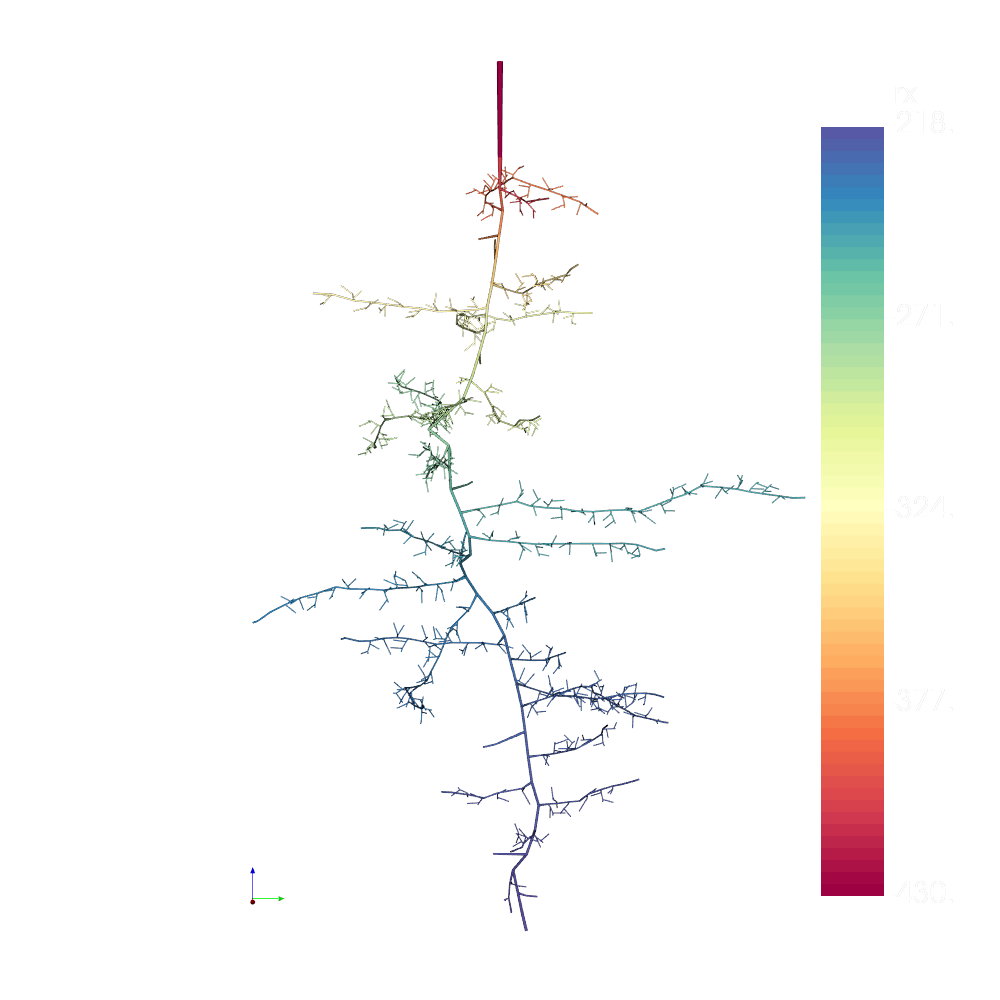
\includegraphics[width=0.99\textwidth]{example6b.png}
\subcaption{Anagallis} \label{fig:xylemfluxa}
\end{subfigure}
\begin{subfigure}[c]{0.5\textwidth}
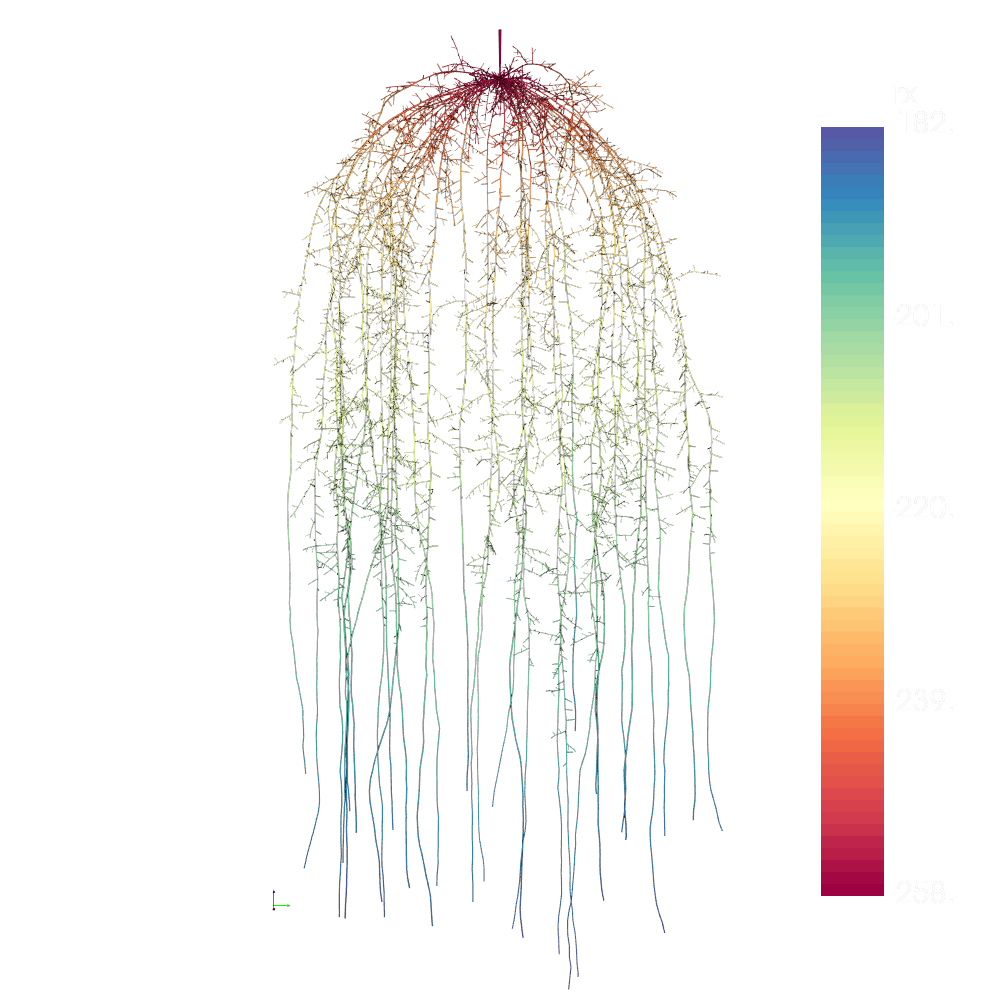
\includegraphics[width=0.99\textwidth]{example6b_2.png}
\subcaption{Maize} \label{fig:xylemfluxb}
\end{subfigure}
\caption{Calculated xylem matric potential (cm)} 
\end{figure}

\subsection{Stomatal modul} \label{ssec:stomatal}

The following example presents the stomatal modul (see file example6e$\_$xylemflux$\_$variable$\_$gs.py). The actual evapotranspiration (ETa) of the plant is determined according to environmental parameters, root and leaf surface, and maximal stomatal conductance (gmax). 
%\lstinputlisting[firstline=1, language=Python, caption=Example 6e]{../examples/example6e_xylemflux_variable_gs.py}
\begin{itemize}

\item[11-19] Part of the parameters that will be used later on.

\item[18-23] The root system (similar to last section). 

\item[21-25] Creation of the plant object, definition of the grid and simulation of the plant growth.

\item[38-42] Set the parameters for the calculation of the actual leaves radial conductivity (gs) and ETa using the equations of [TOADD].

\item[44-48] Get the plant nodes and tips to set the Neumann boundary conditions (i.e. 0 axial flux is set at the plant nod tips (i.e: water only enters/leaves the plant by radial flux)

\item[51] Solve the water flux using the Neumann boundary conditions. The program then loops on the calculation of ETa, xylem potential, and gs until convergence or after having done 1000 loops. p$\_$linit and gmax are respectively the initial leaf xylem potential and initial leaf radial conductivity used in the loop.

\item[52] Calculation of the radial fluxes of each plant segment.

\item[53] Gives an overview of the water fluxes in the plant. If show$\_$matrices = True, the matrices with the axial and radial water fluxes for each plant segment is shown.

\item[62-72] Plots the results (see Figure \ref{fig:stomata} and \ref{fig:stomatb}).

\item[75-78] Creates the VTP file, which can then be opened in Paraview.

\end{itemize}

\begin{figure}
\begin{subfigure}[c]{0.5\textwidth}
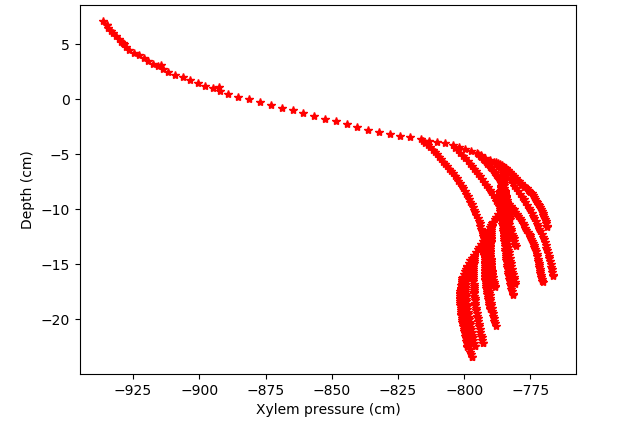
\includegraphics[width=0.99\textwidth]{example6e.png}
\subcaption{Calculated xylem matric potential (cm)} \label{fig:stomata}
\end{subfigure}
\begin{subfigure}[c]{0.5\textwidth}
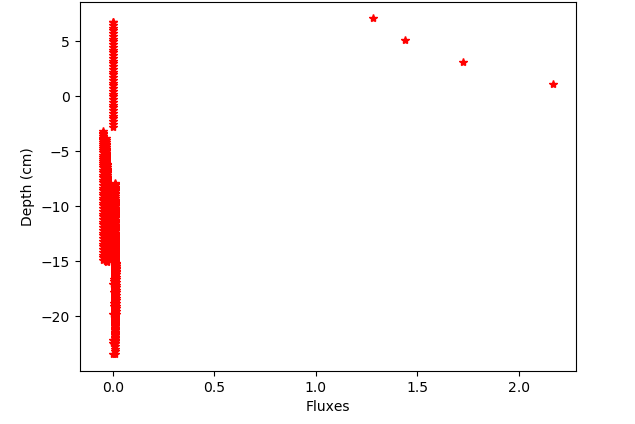
\includegraphics[width=0.99\textwidth]{example6e_2.png}
\subcaption{Radial water fluxes} \label{fig:stomatb}
\end{subfigure}
\caption{xylem potential and radial water fluxes per segment} 
\end{figure}




\subsection{Benchmark examples M3.1 and M3.2} \label{ssec:benchmarks3x}
% 



\subsection{The standard uptake fraction (SUF) and root system conductivity (Krs)} \label{ssec:suf}
% 



\subsection{Plant structure mapped to a macrogrid} \label{ssec:mapped}
% 

After coupling a static root system to a soil model, it is straight forward to couple a growing root system. All there is to do is to update the geometry and the mapping between the grids in every time step. All the work is done by MappedRootSystem.

    
\subsubsection*{Mapping of growing roots and underlying soil} 

In the following we show how the mappings between root system grid and soil grids are updated (see Section \ref{ss:mapping} for the static case). For demonstration we create an animation, where we can see the growth and the dynamic mapping. 

\lstinputlisting[firstline=1, language=Python, caption=Example 7a]{examples/example7a_mapping.py}

\begin{itemize}
\item[8-12] Parameters we might want to modify. 
\item[15-18] Initializes the model.
\item[21-27] Defines a coarse soil grid. If we do not use periodicity we set the domain as confining geometry to the root growth. L27 sets the underlying soil grid.
\item[29-31] Initializes the simulation with an initial simulation run for rs\_age.
\item[33-39] Initializes an VTK animation using the class vp.AnimateRoots, which is work in progress. 
\item[41-59] The simulation loop: L43 performs the simulation, and updates the mappers (no additional steps are needed, everything is updated by pb.MappedRootSystem). L46-52 determines the cell index for each segment for visualization. L54,L L55 makes a SegmentAnalyser object and adds the soil cell indices. L57-L58 updates the animation figure. This is convenient for debugging, and the object vp.AnimateRoots will create an ogg vorbis movie file (which is small and high quality), but for bigger root systems this will be very slow, since a SegmentAnalyser object is created and plotted for each frame (see Section \ref{ssec:animation} for a faster method).
\end{itemize}


\subsection{Model coupling} \label{ssec:coupling}
% 
\subsubsection*{Coupling a static root system to DuMux} \label{sec:dumux_coupling}

Putting the sections \ref{ss:mapping} and \ref{ssec:xylem} together, we can easily set up an example, using the classic sink term in the soil model, similar as in \citep{leitner2014impact} based on \citep{doussan1998modelling}. For solving the Richards equation we use DuMux \citep{koch2020dumux}.

The next example mimics benchmark C12 \citep{schnepf2019call}, but with a static simulated root system. The example must be run out of dumux-rosi (located in dumux-rosi/rosi$\_$benchmarking/python$\_$solver/coupled), otherwise the DuMux Python coupling is not available. 

\lstinputlisting[firstline=1, language=Python, caption=Example 6c]{examples/example6c_coupling.py}

\begin{itemize}
\item[3,4] Add paths for DuMux Python coupling (L3) and Python solvers (L4).

\item[5,6] The direct C++ part of the DuMux binding, and the Python wrapper class. 

\item[17,18]  Defines a sinusoidal function for the collar boundary condition.

\item[21-37] All parameters that are needed for this simulation. L25 decides if periodic boundary conditions are used, or not. L35 states the simulation time, L36 the initial root system age. L37 defines if age dependent root conductivities are used. The rooot conductivities are hard coded in the file root\_conductivities.py, that is imported in L8. Age dependent conductities can be used to mimic root growth in a predefined way, i.e. the root system is already fully grown, but the radial conductivities are turned on during the simulation. 

\item[41-49] Sets up the soil solver (DuMux Python binding from dumux-rosi). 

\item[52-62] Sets up the Xylem model as in Subsection \ref{ssec:xylem}. If the root system is not periodic, a confining geometry is set L54-L58. L62 passes the axial and radial conductivities to the XylemFluxPython object (the function is defined in root\_conductivities.py).

\item[65-70] Coupling between the soil soil and root part is performed by setting the picking function that assigns a cell index to each spatial position L65, and L66. In L67 root segments are cut to the rectangular grid, and in L70 the cell index of the root collar is determined. 

\item[73-77] Initializes the simulation, initially the soil values are the same as the initial conditions (L75).

\item[79-94] First, we calculate the xylem matric potential $rx$ for a given soil matric potential $sx$ (L81) and save the actual collar flux for later analysis (L83). Next, we calculate teh sink (L85) and apply it to the soil model (L86). The soil model is simulated (L87) and the resulting matric potential $sx$ is updated (L88). The simulation takes some time (around 15 minutes), and L90-93 print debugging information and a progress bar. L94 increases the current simulation time. This is needed if age dependent conductivities are used. 

\item[99-111] L99 creates Figure \ref{fig:example6c} and, L102-111 plots uptake and cumulative uptake over time, see Figure \ref{fig:uptake}.
\end{itemize}

\subsubsection*{Coupling a dynamic root system to DuMux with soil feedback} \label{sec:dumux_dyn_coupling}

We modify Example \ref{sec:dumux_coupling}. Using the class MappedRootSystem (as before) it is sufficient to call MappedRootSystem::simulate() to implement real root growth, i.e. to add rs.simulate(dt) in L80. The modified segments and the mapping of new segments is automatically managed (see example7b\_coupling.py). Figure \ref{fig:example7c} shows the root actual uptake over time, with a slightly altered shape compared to \ref{fig:example6c}. Note that the jumps in actual uptake are due to emerging root segments.

In this example soil state does not affect root system growth in any way. We need to add the processes we are interested in (see Section \ref{sec:tropism} and \ref{sec:functional}). For demonstration how to do that, we demonstrate the implementation steps using hydrotropim. Note that the other interactions from Section \ref{sec:functional} could be implemented in the same way. 

In order to use hydrotropism, we need to define a SoilLookUp that accesses the dynamic soil data. We present two approaches: the first uses nearest neighbour interpolation, which is fast but a coarse approximation. The second uses linear interpolation which is more exact, but slower. 

\lstinputlisting[firstline=1, language=Python, caption=Example 7c]{examples/example7c_feedback.py}

We only describe the changes to Section \label{sec:dumux_coupling}:

\begin{itemize}
\item[18-25] We first create a class for nearest neighbour interpolation that extends pb.SoilLookUp. L22 stores a reference to the DuMux soil model. For specialisation of pb.SoilLookUp we need to overwrite the getValue function (L24-25). First we retrieve the cell index by calling $pick$. And, then we return the solution at this cell (in Pascal). Note that the solution is the same for each point within a cell. 
\item[28-41] Secondly, we want to use linear interpolation, which is slower, but more exact. The constructor stores a reference to the soil model (L30-34) the coordinates of the degrees of freedom (i.e. where the points where numerical solution is defined) and calls update(), which fetches the current model solution. Update will be called in after each solving step in the simulation loop. L39-L41 performs the linear interpolation. This is rather slow because the method assumes an unstructured grid, and is not optimized for a structured rectangular grid. 
\item[94-100] We set tropism to hydrotropism (L98) and modify the tropism parameters (L99,100)
\item[102,103] We set the soil, using nearest neighbour or linear interpolation.
\item[120,121] If we use linear interpolation we need to call update to copy the current solution. 
\item[122] Root system simulation, updates geometry and mappers.
\end{itemize}

Figure \ref{fig:example7c} shows that hydrotropism will lead to increased cumulative uptake, because the roots are more evenly distributed. Note that there is a big variation in the results, and for a more profound analysis we would have to make many simulation runs. 

% \begin{figure}
% \begin{subfigure}[c]{1\textwidth}
% 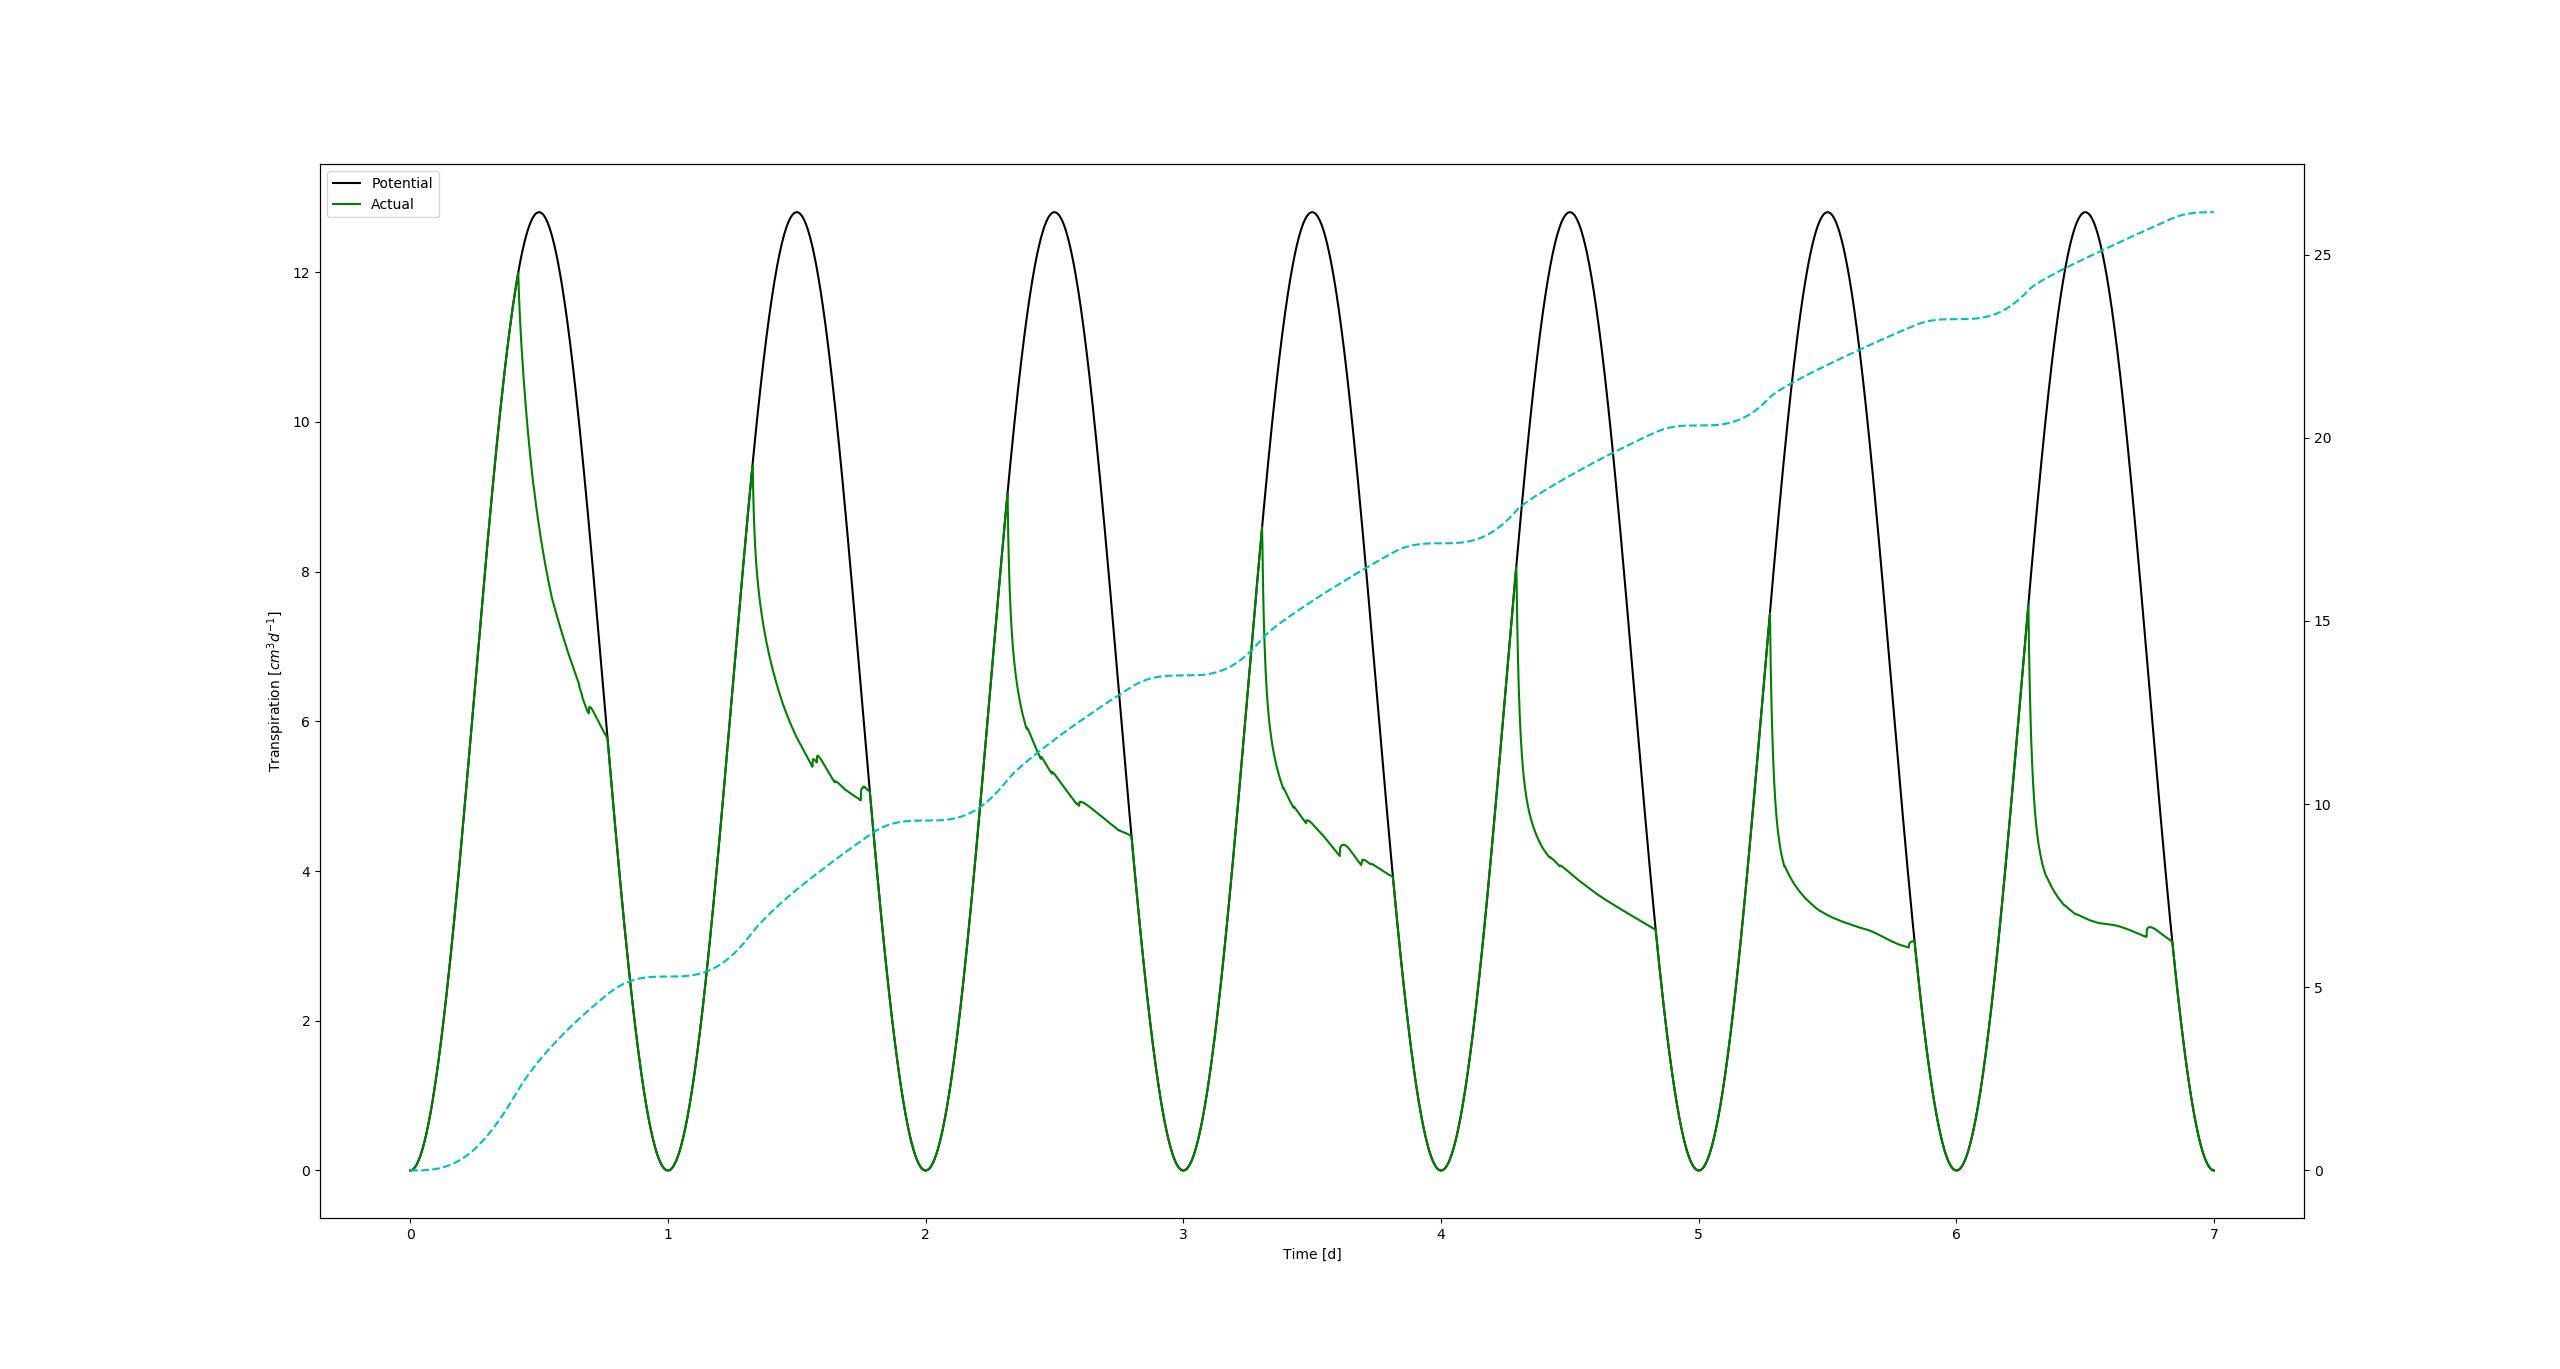
\includegraphics[width=0.99\textwidth]{example7c_no_hydro.png}
% \subcaption{Gravi- and Plagiotropism} \label{fig:example7c}
% \end{subfigure}
% \begin{subfigure}[c]{1\textwidth}
% 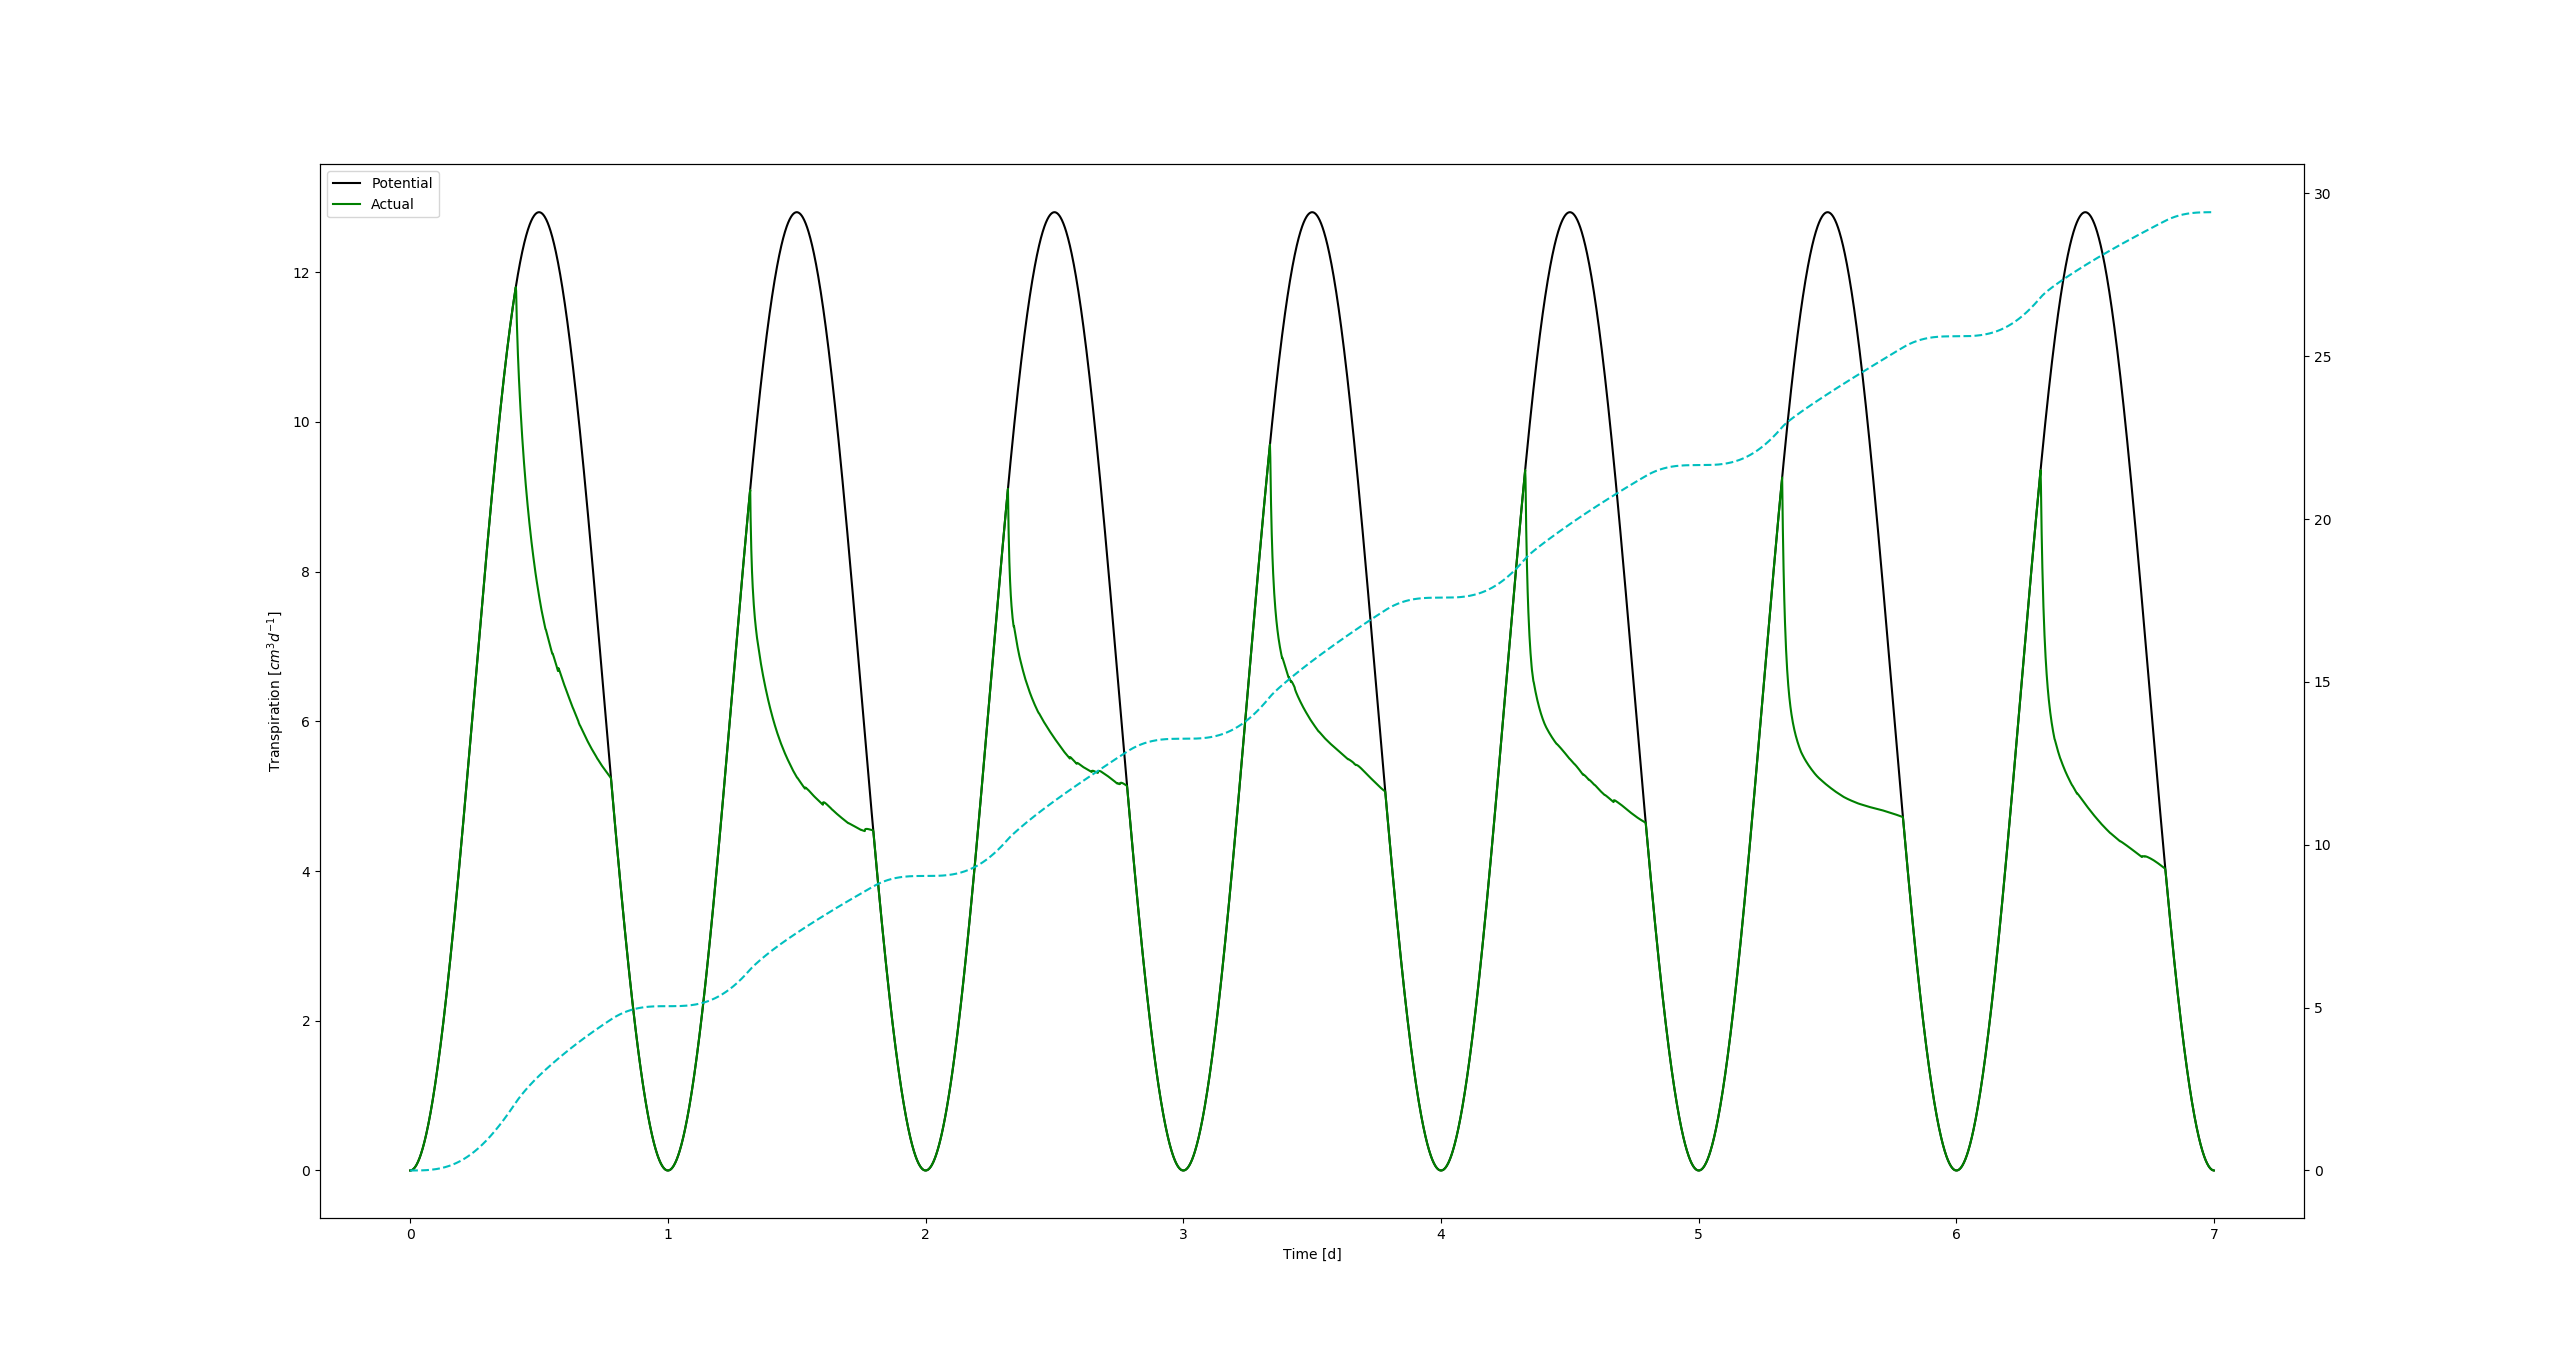
\includegraphics[width=0.99\textwidth]{example7c_simple_hydro.png}
% \subcaption{Hydrotropism} \label{fig:example7c_hydro}
% \end{subfigure}
% \caption{Water uptake a in plant pot} \label{fig:example7c}
% \end{figure}



\subsubsection*{Mimicking root growth}

For a pre-grown root architecture, root growth can be mimicked in a dynamic soil-root interactions simulation using the creation times of the root segments. The root axial conductence $k_x$ is set equal to 0 for ``unborne" root segments with negative age. The root radial conductivity, $k_r$ needs to be equal to 0 (not just a small value) for segments with negative  age. 
The parameter \lstinline{initialT} should be equal to 1 if one wants to mimic growth and equal to the final simulation time if not. 
With respect to solute transport, the diffusion coefficient needs to be very small  for unborn segments (?).



\subsubsection*{Estimating the hydraulic conductivity drop in the rhizosphere} \label{sec:hydro_rhizo}

The resolution of the soil grid is often too coarse to catch small-scale rhizosphere gradients in hydraulic conductivity near the roots. The consequence is that root water uptake is overestimated. One solution would be (adaptive) grid refinement, however at the cost of computation time and the validity of the line-source assumption that we take for the roots in our setup. 
An alternative solution is to keep the coarse soil grid resolution and estimate the soil water potential at the root-soil interface. We implemented two ways of doing so within dumux-rosi. Firstly, we split the volume of each soil control element between the root segments that lie inside it, and assign a soil cylinder around each root segment. In each soil cylinder, the 1D radially symmetric Richards equation is solved and coupled to the macroscopic scale in a mass conservative way via the outer boundary conditions of the soil cylinders. 

Another approach is described in this example and follows the approach described in \cite{Schroeder2008}. Each root segment inside a soil control element of volume $V_s$ has an assigned ``rhizosphere soil volume" equal to $$V_{rhizo} = k V_s,$$ where the weighting factor $k$ is the fraction of the root segment volume $V_{rs}$ relative to the overall volume of roots $V_{rst\textsc{}}$ inside $V_s$, $k=\frac{V_{rs}}{V{rst}}$. 
From this, the outer radius of the rhizosphere cylinder is computed by 
$$r_{out}=\sqrt{\frac{V_{rhizo}+V_{rs}}{\pi l}},$$ where $l$ is the root segment length. 


Then the flux at the root-soil interface is estimated based on the analytical solutions of the 1D radially symmetric Richards equation. Based on the steady-rate assumption and using the matric flux potential $\Phi(h_c)=\int_{-\infty}^{h_c}  K(h) dh$ that linearizes the Richards equation, the radial matric flux potential profiles for non-stressed and stressed conditions are given by 
\begin{multline}
\Phi(r)=\Phi_{r_{out}} + (q_{root}r_{root}-q_{out}r_{out})\left[ \frac{r^2/r_{root}^2}{2(1-\rho^2)} + \frac{\rho^2}{1-\rho^2}\left(\text{ln}  \frac{r_{out}}{r}-\frac{1}{2} \right) \right] \\\ + q_{out}r_{out} \text{ln} \frac{r}{r_{out}}
\end{multline}
and 
\begin{multline}
\Phi(r) = \left(\Phi_{r_{out}} - \Phi_{r_{root}} + q_{out}r_{out}\text{ln} \frac{1}{\rho}\right)\frac{r^2/r_{root}^2 - 1 + 2\rho^2 \text{ln}  r_{root}/r}{\rho^2 -1 + 2\rho^2 ln 1/\rho} \\\ + q_{out}r_{out}\text{ln} \frac{r}{r_{root}} + \Phi_{root},
\end{multline}
where $\rho=\frac{r_{out}}{r_{root}}$, $r_{root}$ is the root radius, $r_{out}$ is the outer radius, $q_{root}$ is the flux prescribed at the root-soil interface, $q_{out}$ is the flux at the outer boundary.

Given the soil matric potential at the outer boundary, and either the flux (non-stressed conditions) or soil matric potential (stressed) at the root-soil interface, the solution computes the radial matrix flux potential profile, and from the matric flux potential, the soil matric potential can be inferred. The soil matric potential at the outer boundary is taken to be the macroscopic soil matric potential value of the given soil control element at the given time step. The water flux at the outer boundary, $q_{out}$, is computed such that the sum of the fluxes at the outer boundaries of the rhizosphere cylinders is equal to the net flux into or out of the given soil control element, $q_{V_s}$, at a given time step, and $$q_{out}=k q_{V_s}$$, where $k$ is the same weighting factor as described above. However, setting the outer flux to zero is sufficient in most cases, as there is redistribution after every time step.  

We start the simulation by computing the root water uptake according to the classical (see section \ref{s:coupling}). 
Then, for every root segment and at every time step, we check whether the matric flux potential at the root-soil interface is positive or negative. In case the matric flux potential is positive, root water uptake follows non-stressed conditions, and the sink term is left according to the classical approach. In case the matric flux potential is negative, root water uptake follows stressed conditions and the soil matric potential at the root-soil interface is equal to the wilting point. The water flux from soil into the root is computed by numerically approximating the soil matric potential gradient at the root-soil interface and multiplying this by the hydraulic conductivity.

Finally, the flux at the root-soil interface is the maximum of the classical and steady-rate approximation value. This makes sure that hydraulic redistribution (i.e. flow from roots to soil) is still possible. 

Listing X shows the code of file ``coupled\_c12\_schroeder.py".
%\lstinputlisting[firstline=1, language=Python, caption=Example 6a]{../examples/example6a_mapping.py}

\begin{itemize}
\item[106-110] Root xylem potentials are computed based on the current soil (at first call) or rhizosphere (from second call onwards) water potentials. 
\item[112] Rhizosphere soil water potentials are updated from the current soil and xylem water potentials using the steady-rate assumption. 
\item[113] For each root segment, the water fluxes are computed from the current xylem and rhizosphere water potentials. 
\item[115] For the soil control element, sum of root water uptake over all root segments inside a given soil control element is computed. 
\item[127] The fluxes are set as sources in the soil problem (Richards equation)
\item[131] Soil problem is solved for one time step. 
\end{itemize}

   
Listing Y shows the C++ code for the computation of matric potential at the root-soil interface according to \citep{Schroeder2008}. The fluxes are then computed according to the pressure differences...
%\lstinputlisting[firstline=1, language=Python, caption=Example 6a]{../examples/example6a_mapping.py}

\begin{itemize}
\item[234] Computation of the matrix flux potential according to the non-stressed equation. 
\item[237] For positive mfp (no stress), the soil matric potential at the root-soil interface is set to the corresponding value.
\item[240] For negative mfp (stress), the soil matric potential at the root-soil interface is set equal to the wilting point. 
\item[245] If the xylem water potential is larger than the root-soil interface potential, root-soil interface potential is set equal to the xylem water potential (no flux). 
\item[248] On the macroscopic scale, flow of water from root to soil is enabled. 
\end{itemize}


Figure \ref{fig:schroeder} the transpiration rate and cumulative transpiration computed based on the steady-rate assumption for the case of a clay soil. 

% \begin{figure}
% %\begin{subfigure}[c]{1\textwidth}
% 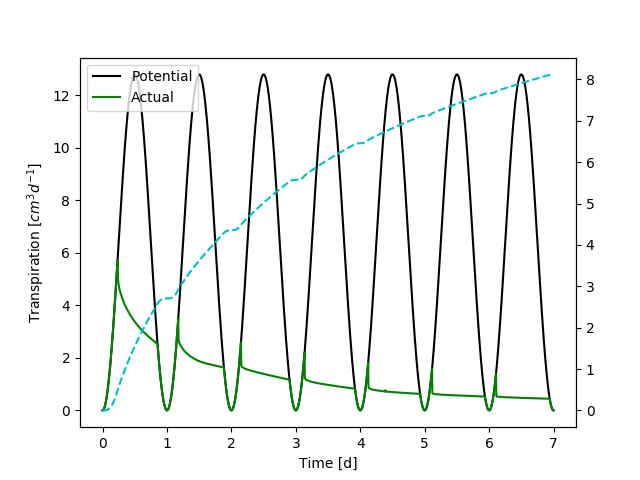
\includegraphics[width=0.99\textwidth]{clay_schroeder.png}
% %\subcaption{Gravi- and Plagiotropism} \label{fig:example7c}
% %\end{subfigure}
% %\begin{subfigure}[c]{1\textwidth}
% %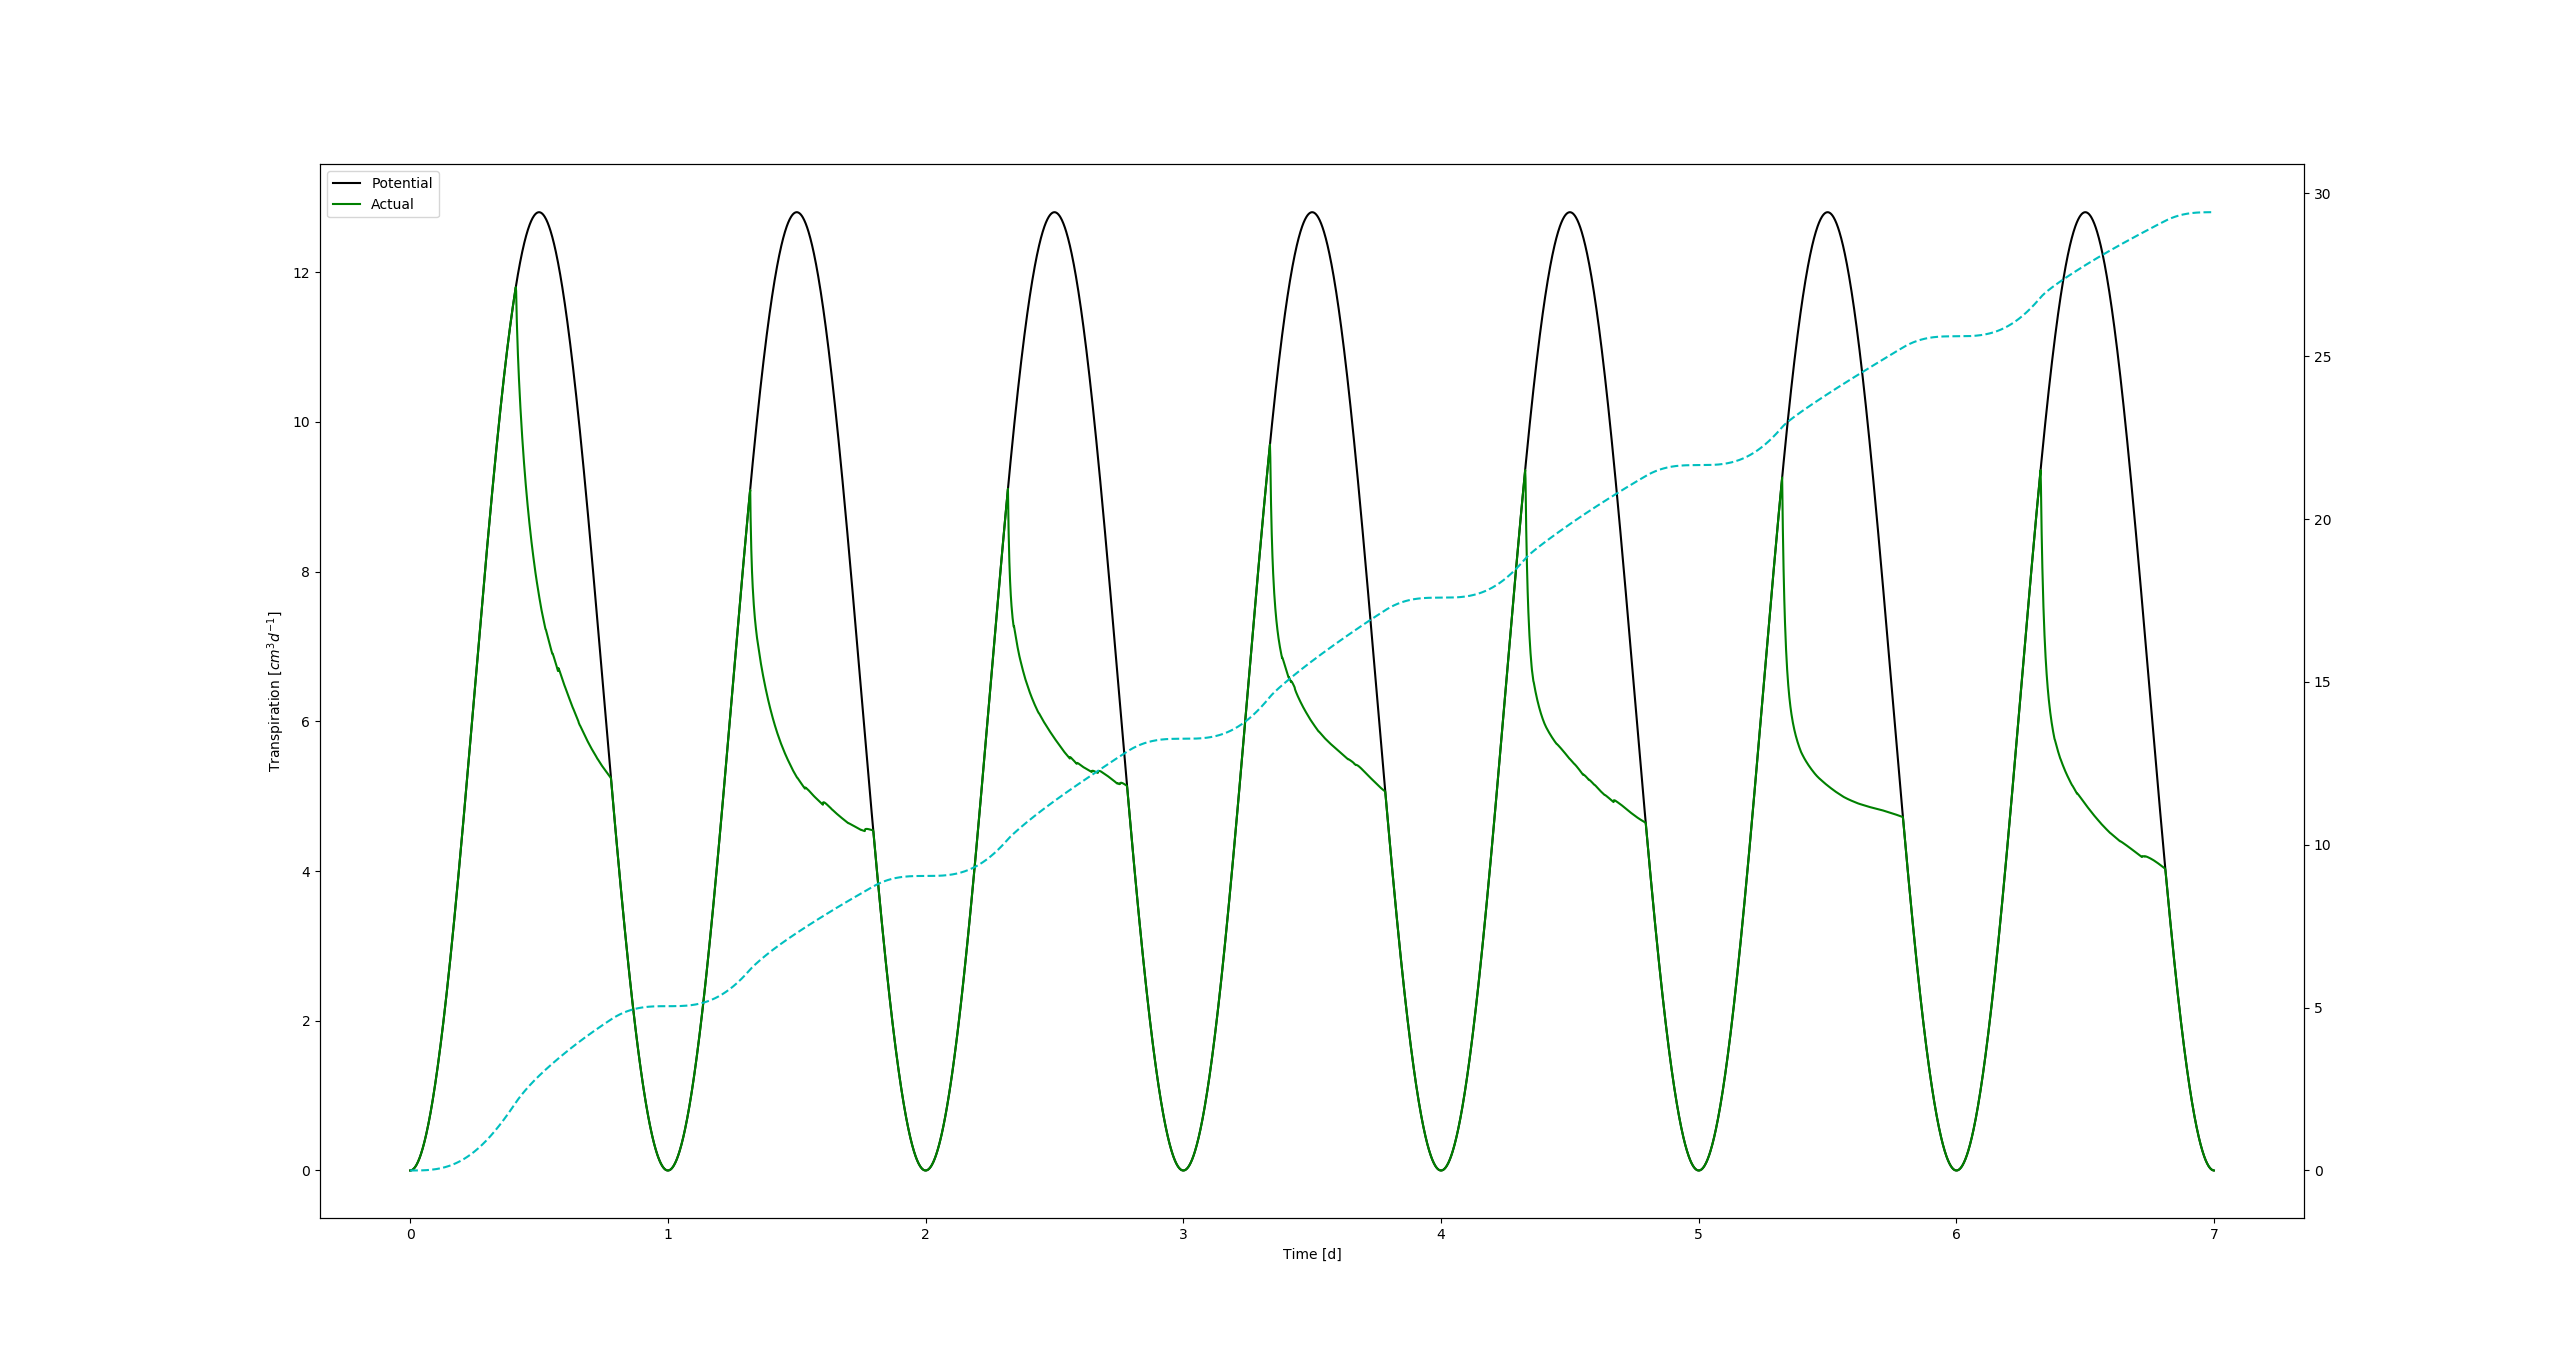
\includegraphics[width=0.99\textwidth]{example7c_simple_hydro.png}
% %\subcaption{Hydrotropism} \label{fig:example7c_hydro}
% %\end{subfigure}
% \caption{Transpiration rate and cumulative transpiration computed based on the steady-rate assumption.} \label{fig:schroeder}
% \end{figure}








\subsection{Stomatal model} \label{ssec:stomatal}
% \subsubsection*{Stomatal model} \label{ssec:stomatal}

The following example presents the stomatal modul (see file example6e$\_$xylemflux$\_$variable$\_$gs.py). The actual evapotranspiration (ETa) of the plant is determined according to environmental parameters, root and leaf surface, and maximal stomatal conductance (gmax). 
%\lstinputlisting[firstline=1, language=Python, caption=Example 6e]{../examples/example6e_xylemflux_variable_gs.py}
\begin{itemize}

\item[11-19] Part of the parameters that will be used later on.

\item[18-23] The root system (similar to last section). 

\item[21-25] Creation of the plant object, definition of the grid and simulation of the plant growth.

\item[38-42] Set the parameters for the calculation of the actual leaves radial conductivity (gs) and ETa using the equations of [TOADD].

\item[44-48] Get the plant nodes and tips to set the Neumann boundary conditions (i.e. 0 axial flux is set at the plant nod tips (i.e: water only enters/leaves the plant by radial flux)

\item[51] Solve the water flux using the Neumann boundary conditions. The program then loops on the calculation of ETa, xylem potential, and gs until convergence or after having done 1000 loops. p$\_$linit and gmax are respectively the initial leaf xylem potential and initial leaf radial conductivity used in the loop.

\item[52] Calculation of the radial fluxes of each plant segment.

\item[53] Gives an overview of the water fluxes in the plant. If show$\_$matrices = True, the matrices with the axial and radial water fluxes for each plant segment is shown.

\item[62-72] Plots the results (see Figure \ref{fig:stomata} and \ref{fig:stomatb}).

\item[75-78] Creates the VTP file, which can then be opened in Paraview.

\end{itemize}

\begin{figure}
\begin{subfigure}[c]{0.5\textwidth}
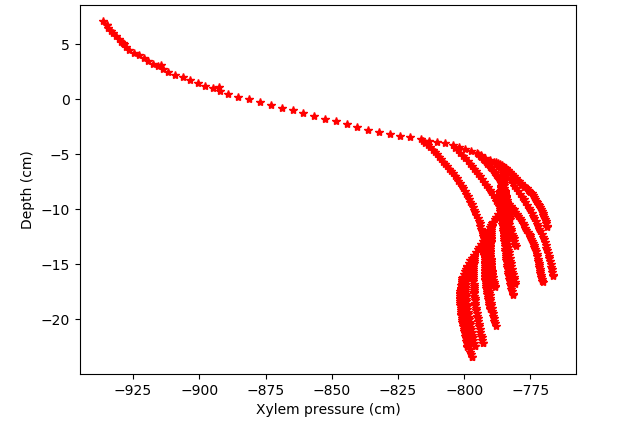
\includegraphics[width=0.99\textwidth]{example6e.png}
\subcaption{Calculated xylem matric potential (cm)} \label{fig:stomata}
\end{subfigure}
\begin{subfigure}[c]{0.5\textwidth}
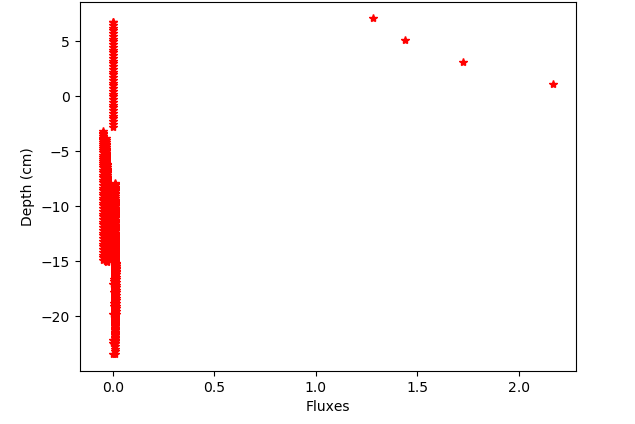
\includegraphics[width=0.99\textwidth]{example6e_2.png}
\subcaption{Radial water fluxes} \label{fig:stomatb}
\end{subfigure}
\caption{xylem potential and radial water fluxes per segment} 
\end{figure}

\subsubsection*{Coupling a static root system to DuMux} \label{sec:dumux_coupling}

Putting the sections \ref{ss:mapping} and \ref{ssec:xylem} together, we can easily set up an example, using the classic sink term in the soil model, similar as in \citep{leitner2014impact} based on \citep{doussan1998modelling}. For solving the Richards equation we use DuMux \citep{koch2020dumux}.

The next example mimics benchmark C12 \citep{schnepf2019call}, but with a static simulated root system. The example must be run out of dumux-rosi (located in dumux-rosi/rosi$\_$benchmarking/python$\_$solver/coupled), otherwise the DuMux Python coupling is not available. 

\lstinputlisting[firstline=1, language=Python, caption=Example 6c]{examples/example6c_coupling.py}

\begin{itemize}

\item[3,4] Add paths for DuMux Python coupling (L3) and Python solvers (L4).

\item[5,6] The direct C++ part of the DuMux binding, and the Python wrapper class. 

\item[17,18]  Defines a sinusoidal function for the collar boundary condition.

\item[21-37] All parameters that are needed for this simulation. L25 decides if periodic boundary conditions are used, or not. L35 states the simulation time, L36 the initial root system age. L37 defines if age dependent root conductivities are used. The rooot conductivities are hard coded in the file root\_conductivities.py, that is imported in L8. Age dependent conductities can be used to mimic root growth in a predefined way, i.e. the root system is already fully grown, but the radial conductivities are turned on during the simulation. 

\item[41-49] Sets up the soil solver (DuMux Python binding from dumux-rosi). 

\item[52-62] Sets up the Xylem model as in Subsection \ref{ssec:xylem}. If the root system is not periodic, a confining geometry is set L54-L58. L62 passes the axial and radial conductivities to the XylemFluxPython object (the function is defined in root\_conductivities.py).

\item[65-70] Coupling between the soil soil and root part is performed by setting the picking function that assigns a cell index to each spatial position L65, and L66. In L67 root segments are cut to the rectangular grid, and in L70 the cell index of the root collar is determined. 

\item[73-77] Initializes the simulation, initially the soil values are the same as the initial conditions (L75).

\item[79-94] First, we calculate the xylem matric potential $rx$ for a given soil matric potential $sx$ (L81) and save the actual collar flux for later analysis (L83). Next, we calculate teh sink (L85) and apply it to the soil model (L86). The soil model is simulated (L87) and the resulting matric potential $sx$ is updated (L88). The simulation takes some time (around 15 minutes), and L90-93 print debugging information and a progress bar. L94 increases the current simulation time. This is needed if age dependent conductivities are used. 

\item[99-111] L99 creates Figure \ref{fig:example6c} and, L102-111 plots uptake and cumulative uptake over time, see Figure \ref{fig:uptake}.

\end{itemize}

% \begin{figure}
% \begin{subfigure}[c]{0.5\textwidth}
% 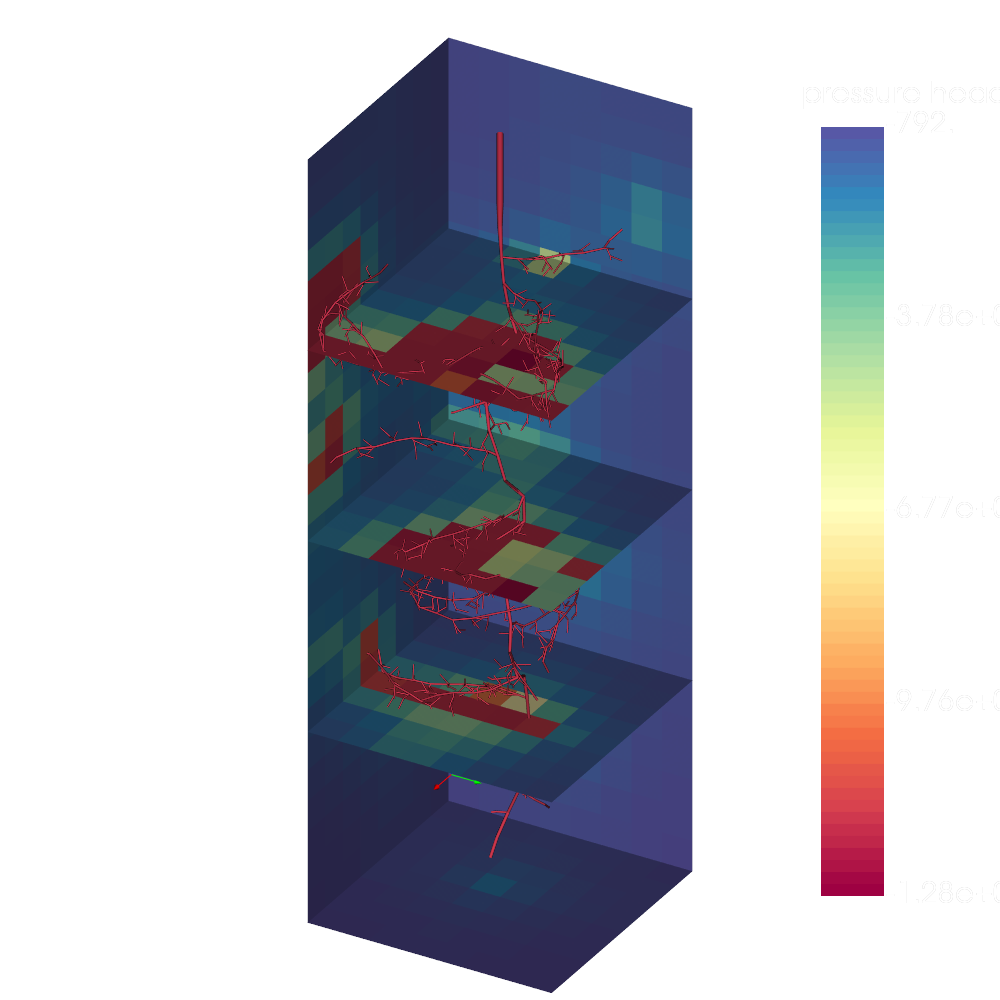
\includegraphics[width=0.99\textwidth]{example6c.png}
% \subcaption{Confined} \label{fig:example6c}
% \end{subfigure}
% \begin{subfigure}[c]{0.5\textwidth}
% 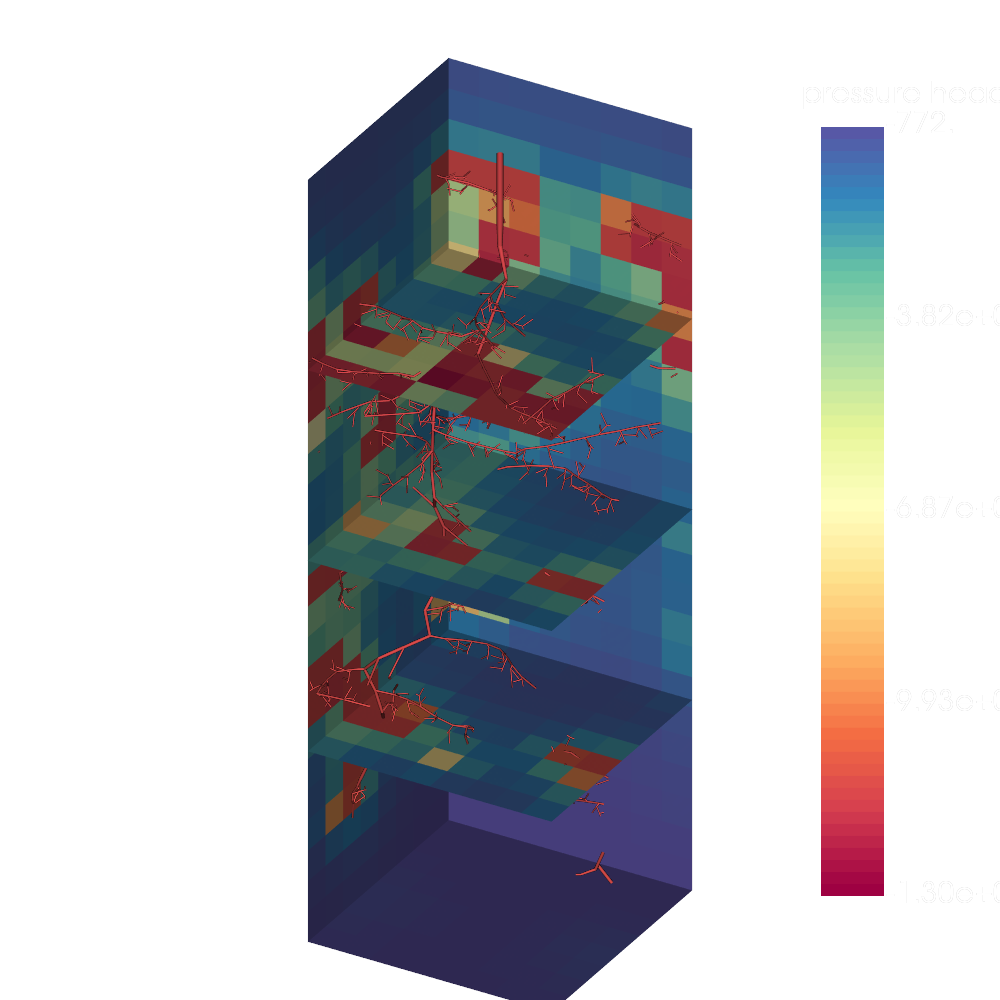
\includegraphics[width=0.99\textwidth]{example6c_periodic.png}
% \subcaption{Periodic boundary condtions} \label{fig:example6c_peridodic}
% \end{subfigure}
% \caption{Water depletion due to root uptake after one week. } \label{fig:example6c}
% \end{figure}

With above code we can compare total root system water uptake in a container, with the uptake if periodic boundary conditions are used. While the first scenario reflects the situation in a plant pot, periodic boundary conditions reflect the situation when the plant grows in the field, where the planting distance is approximately the domain size. Figure \ref{fig:uptake} shows both situations, showing that the boundary conditions will strongly affect total water uptake, because roots are less evenly distributed in the pot scenario and water redistribution is impeded by the pot boundaries.

% \begin{figure}
% \begin{subfigure}[c]{1\textwidth} 
% 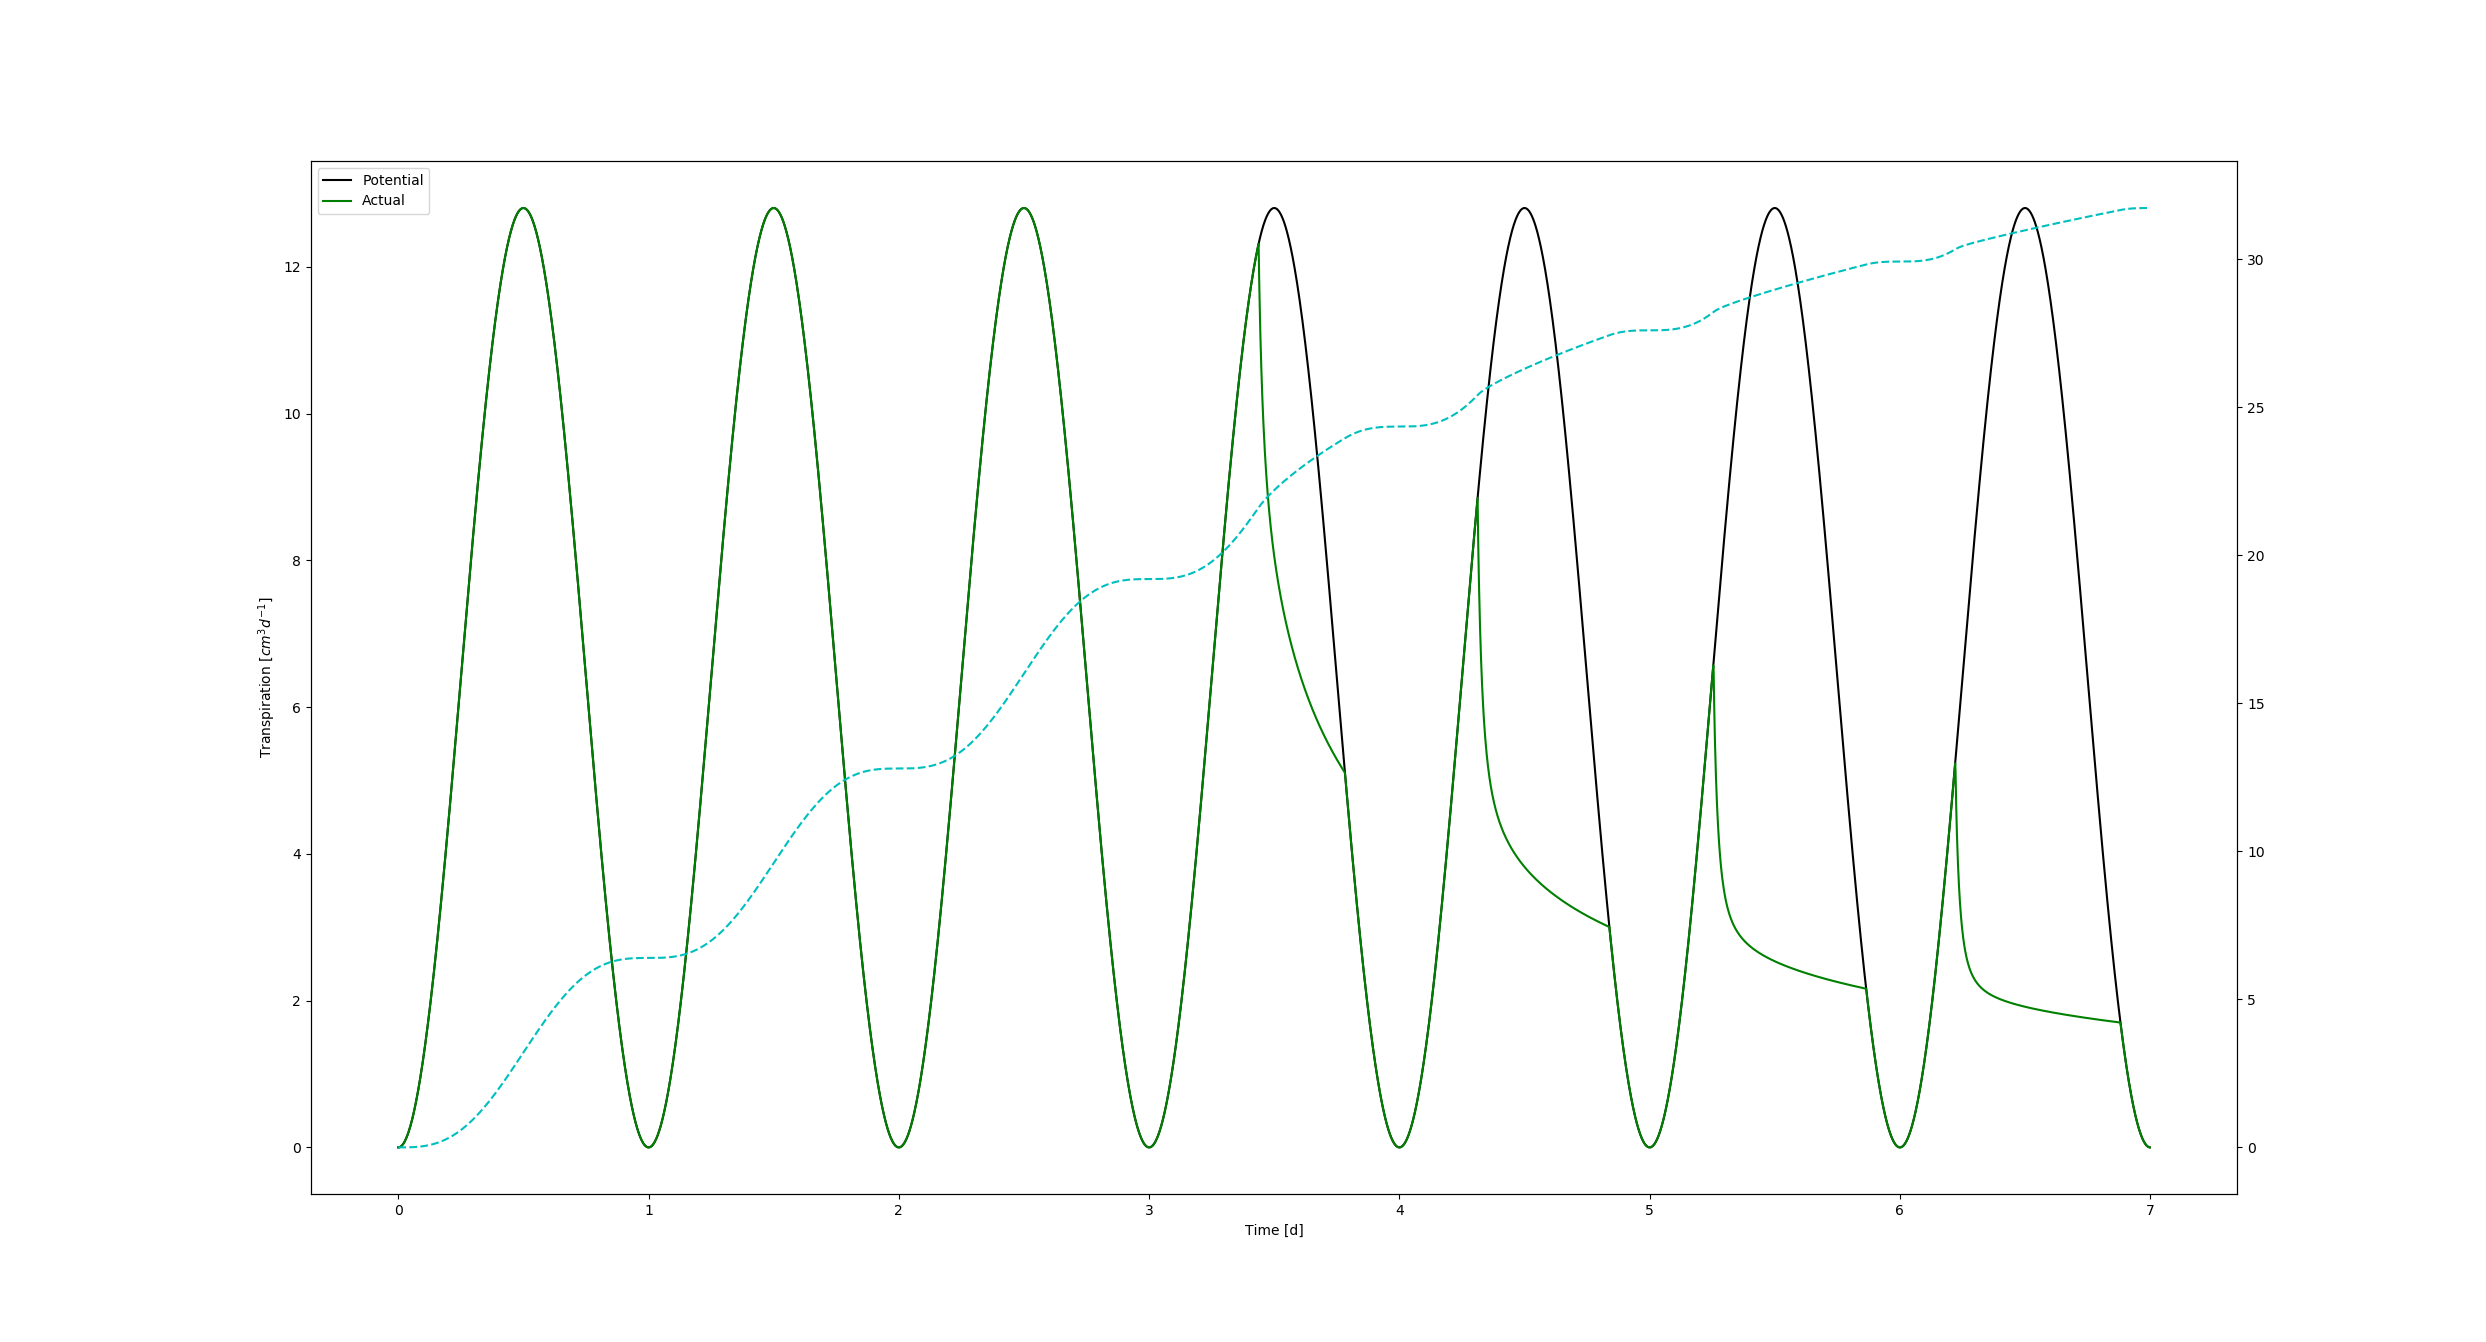
\includegraphics[width=0.99\textwidth]{Figure6c.png}
% \subcaption{Confined} \label{fig:uptake_confined}
% \end{subfigure}
% \begin{subfigure}[c]{1\textwidth}
% 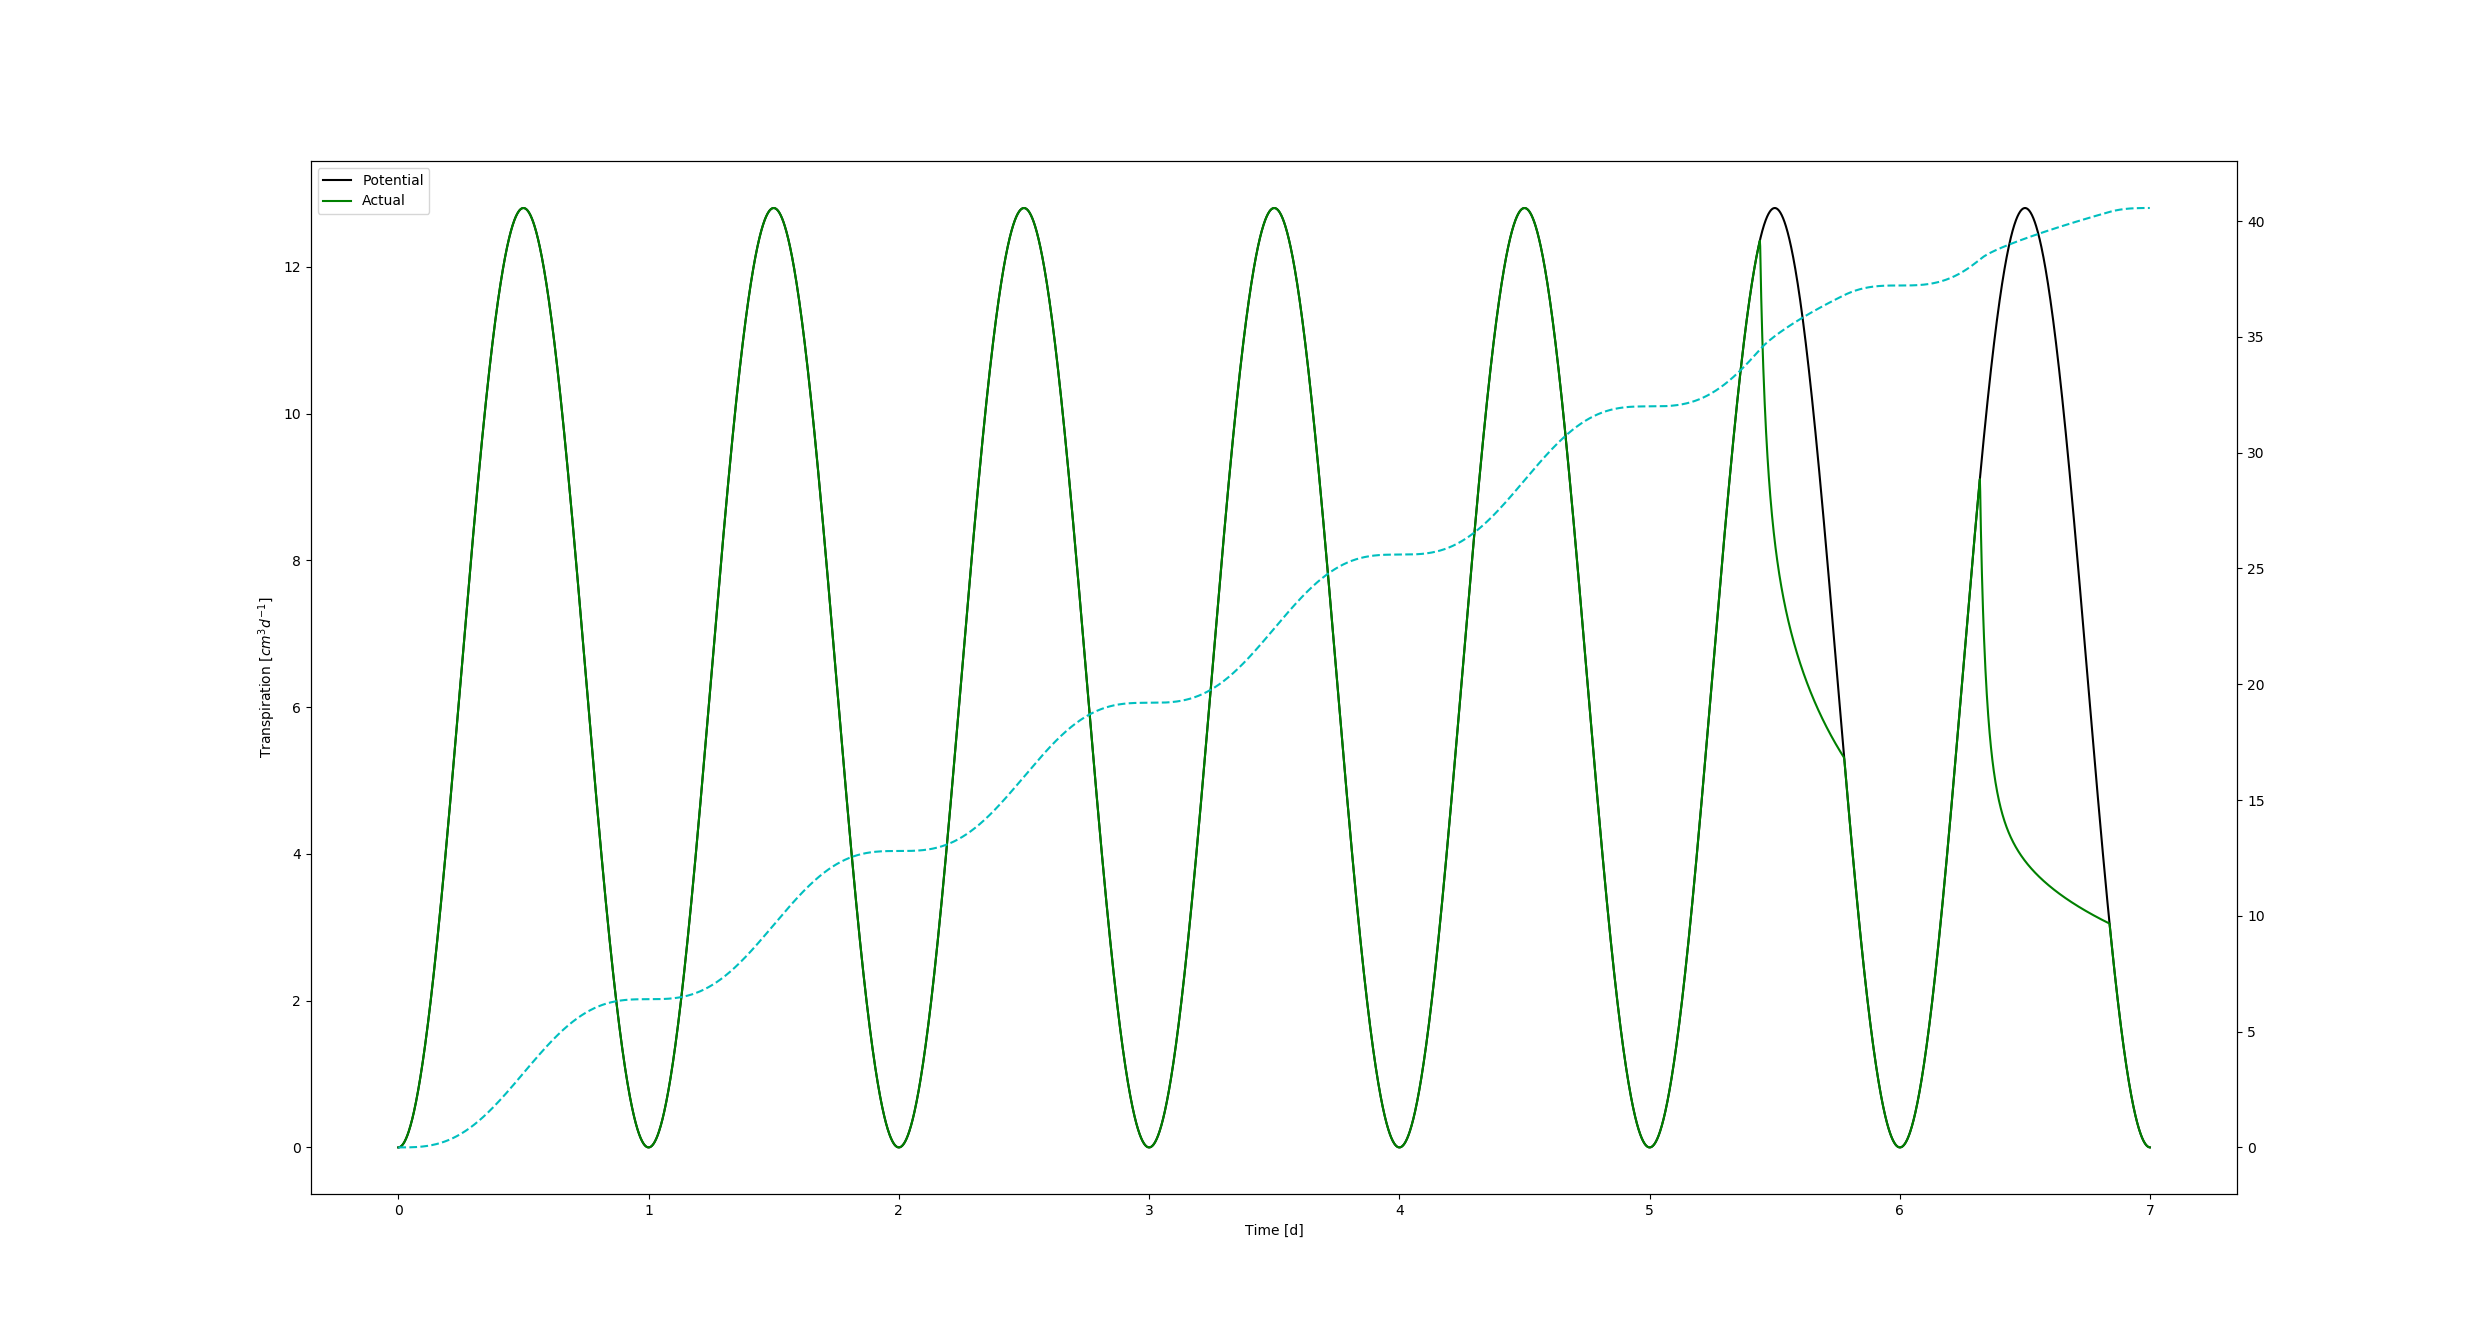
\includegraphics[width=0.99\textwidth]{Figure6c_periodic.png}
% \subcaption{Periodic boundary condtions} \label{fig:uptake_peridodic}
% \end{subfigure}
% \caption{Water uptake and cumulated uptake} \label{fig:uptake}
% \end{figure}



\newpage
\section{Contributing} \label{sec:contributing}

\subsection{Coding style} \label{ssec:coding_style}




\subsection{Todos} \label{ssec:todos}

Topics that are not covered yet or should be improved

\begin{itemize}

\item Elongation rate according to Moacir et al.

\item Delay based, versus length based lateral emergance.

\item Better branching probability example.

\item Periodicity without DuMux coupling, but with a soil 3d grid (untested, and an example is missing)

\item Carbon limited root system growth

\item Direct vtk animation with vp.AnimateRoots (under development...)

\item The DuMux binding and MPI (probably belongs to dumux-rosi)


\end{itemize}






\newpage
\bibliographystyle{apalike} 
\bibliography{latex/references} 


\end{document}
